% !TeX root = ../main.tex

\chapter{在双喷注末态事例中寻找超出标准模型的新物理}
\label{cha:Dijet}



许多超出标准模型~\cite{qstar1,qstar2,zprime1,zprime3,wprime1,Chizhov:2009fc,Chizhov:2010jg,DM1,DM2,DM3,qbh1,qbh2,RS1,RS2}
的新物理预言了能与标准模型中夸克($q$)或者胶子($g$)耦合的新的重粒子的存在,
而这些新粒子如果存在的话能通过高能质子对撞产生,并衰变成两个能量很高的夸克或者胶子,
以两个喷注即dijet的形式被探测器探测到,图~\ref{fig:Dijet1}~示为过程所对应的费曼图。
在标准模型中,dijet末态事例主要来自于QCD过程,
而QCD预言的dijet的不变质量谱$m_{jj}
$\footnote{自然单位制下,两个物理对象的不变质量定义为$m_{12}=\sqrt{(E_1+E_2)^2-(\vec{p_1}+\vec{p_2})^2}$,其中($E_1$,$\vec{p_1}$)、($E_2$,$\vec{p_2}$)分别为两个物理对象的能量和动量。}
是平滑下降的,
若是有一个非标准模型的新粒子衰变到夸克或者胶子,在QCD预言的平滑下降的$m_{jj}$上便会出现一个小鼓包,
对应于新粒子的质量,可以以此为手段来寻找新物理~\cite{UA3}。

\begin{figure}
  \begin{center}
    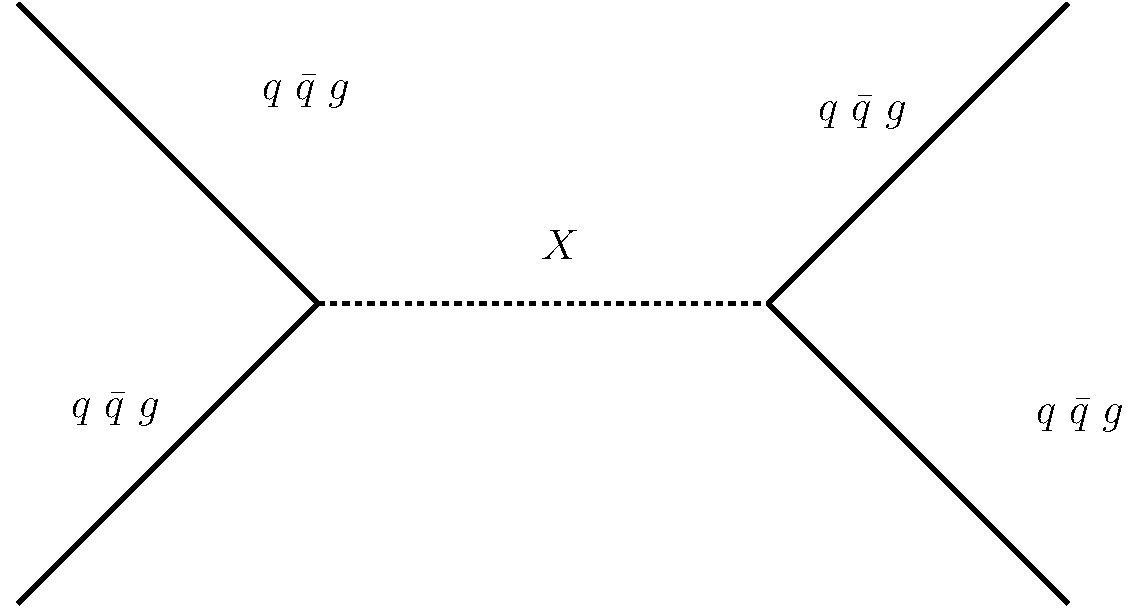
\includegraphics[width=0.5\textwidth]{figuresTHE/SChl.pdf}
  \end{center}
  \caption{
新粒子的产生模式。其中X表示新粒子。
}
    \label{fig:Dijet1}
\end{figure}


\section{研究背景}
\label{sec:DijetBKG}


最早的双喷注共振态新物理的寻找是1988年由UA1实验引导的,
当时的质子反质子对撞的质心系能量为0.63TeV,数据总积分亮度为0.26$pb^{-1}$,
寻找的质量区间为0.07-0.3TeV,并使用领头阶(Leading order, LO) QCD 做本底估计,
测量发现数据与标准模型的预期一致~\cite{UA1}。
在总积分亮度达到0.49$pb^{-1}$之后又更新了一次结果,
未发现超出标准模型的新粒子~\cite{UA2}。随后在1990年,
同样是质子反质子对撞实验,CDF实验使用总积分亮度为0.026$pb^{-1}$质心系能量为1.8TeV的数量,
使用同样的方法进行了寻找,寻找的质量区间上限有了提升,达到0.06-0.5TeV,未发现超出标准模型的新粒子~\cite{CDF1}。
紧接着UA2实验在总积分亮度提升到4.7$pb^{-1}$之后,使用函数拟合的方法做本底估计进行了寻找,
未发现新粒子~\cite{UA3}。在之后的二十年内CDF实验UA2实验和D0实验陆续更新了不同亮度的寻找结果,
仍未发现新粒子~\cite{CDF2,UA4,CDF3,CDF4,D01,CDF5},其中2009年CDF实验中~\cite{CDF5}质心系能量为1.96TeV,总积分亮度达到了1130$pb^{-1}$。

从2010年开始,随着LHC的成功运转,使用高能质子与质子对撞,
在$Run\_1$计划期间,质心系能量得到显著的提升,达到了7TeV,
ATLAS实验和CMS实验在此基础上更新了更宽的质量区间的寻找结果~\cite{ATLASDijet1,ATLASDijet2,ATLASDijet3,ATLASDijet4,CMSDijet1,CMSDijet2},
其中 ATLAS合作组在2013 年的实验结果中使用的数据总积分亮度达到了4.8$fb^{-1}$,寻找的质量区间上限达到了约4.0TeV~\cite{ATLASDijet4},
CMS合作组在2011年的实验结果中数据总积分亮度为2.9$pb^{-1}$,寻找的质量区间上限在2TeV左右~\cite{CMSDijet2},未发现新粒子。
随后在质心系能量升级到 8TeV之后,ATLAS实验和CMS实验分别在2015年和2013年更新了新的寻找结果~\cite{ATLASDijet5,CMSDijet3},
总积分亮度分别达到了20.3$fb^{-1}$和4.0$fb^{-1}$,搜索的质量上限分别在4.5TeV和4.8TeV,也未发现新粒子。

接着在LHC升级改造之后,在$Run\_2$计划期间,将质心系能量提升到了13TeV,并且总积分亮度也有显著提高,
于是ATLAS实验和CMS实验在最近几年更新了更为丰富的实验结果~\cite{ATLASDijet6,ATLASDijet7,ATLASDijet8,ATLASDijet9,CMSDijet4,CMSDijet5,CMSDijet6},
其中 ATLAS合作组在2017年的实验结果中总积分亮度达到了37$fb^{-1}$,实现了更高质量区间1.1-8.2TeV的寻找~\cite{ATLASDijet8};
而且在2018年还对衰变末态中的一个或者两个jet被标定为b-jet的新粒子进行了搜索~\cite{ATLASDijet9},
如果新粒子与$b$夸克的耦合强度比较大,并衰变到$b\bar{b}$、$bq$或者$bg$对,则对衰变末态进行b-jet标定($b$-tagging)可以显著的提升寻找这类新粒子的灵敏度,
同年,CMS合作组也更新了质心系能量为8TeV下含味标定末态的新粒子的搜索结果~\cite{CMSDijet7};
同时,CMS合作组在2018年的实验结果中总积分亮度达到了36$fb^{-1}$,搜索的质量上限也提升到了接近8TeV~\cite{CMSDijet6},都未发现新粒子。

%7TeV~\cite{ATLASDijet1,ATLASDijet2,ATLASDijet3,ATLASDijet4,CMSDijet1,CMSDijet2}
%8TeV~\cite{ATLASDijet5,CMSDijet3,CMSDijet7}
%13TeV~\cite{ATLASDijet6,ATLASDijet7,ATLASDijet8,ATLASDijet9,CMSDijet4,CMSDijet5,CMSDijet6}
%如果新粒子与$b$夸克的耦合强度比较大,并衰变到$b\bar{b}$、$bq$或者$bg$对,则在衰变末态中对jet进行$b$夸克标定($b$-tagging)可以显著的提升寻找这类新粒子的灵敏度。
%这个分析通过搜索$m_{jj}$上局部突出的小鼓包来寻找新粒子,其中$m_{jj}$是事例中两个横动量($p_{T}$)最高的jet的不变质量谱,所搜索的质量谱包括所有类型的jet都包含在内的情形和其中一个jet或者全部的两个jet被标定为$b$夸克的情形。
%在以前的强子对撞实验中,双喷注共振态的寻找覆盖了$110GeV$到$1.4TeV$的质量区间~\cite{UA1_dijet,UA2_dijet,cdf_dijet,d0_dijet}。而在LHC上,最新的研究將搜索的质量区间上限提升到了$7.5TeV$~\cite{EXOT-2016-21,CMS-EXO-16-056},由于LHC上触发器和数据收集系统的约束,搜索的质量区间下限也在$1TeV$以上。对于搜索质量区间在$TeV$以下的双喷注共振态,通过使用更加复杂的触发器或者分析策略,LHC上也有了一些结果~\cite{EXOT-2016-20,EXOT-2018-05,EXOT-2017-01,CMS-EXO-16-030,CMS-EXO-17-001,CMS-EXO-17-024}。同样对于新共振态的衰变末态中包含$b$ jet的情形,也有相关的研究工作~\cite{EXOT-2016-33,CMS-EXO-16-057}。
LHC整个$Run\_2$计划中可用于物理分析的数据总积分亮度高达139$fb^{-1}$,为了更近一步的提高dijet末态新粒子的搜索灵敏度和部分新物理模型的排除上限,
在这个分析中,我们使用ATLAS探测器在整个$Run\_2$计划期间且质心系能量为$\sqrt{s}=13TeV$下收集到的总积分亮度为$139fb^{-1}$的数据,
通过在dijet末态事例的不变质量谱$m_{jj}$上搜寻局部突出的共振峰,在TeV量级的高质量区间寻找超出标准模型的新粒子。
其中$m_{jj}$为事例中两个横动量($p_{T}$)最高的jet的不变质量谱,搜索的信号区有三个,
包括不区分末态jet味信息的全包含信号区,以及区分末态jet味信息的信号区:末态两个横动量最高的jet中一个被标定为b-jet的1b信号区和其中的两个jet都被标定为b-jet的2b信号区。
搜索的基准信号模型包括激发态夸克模型$q^*$($q=(u,d,c,s,b)$)~\cite{qstar1,qstar2};重规范玻色子模型$Z\prime$和$W\prime$~\cite{zprime1,zprime3,wprime1};
手征激发态模型$W^*$~\cite{Chizhov:2009fc,Chizhov:2010jg};
暗物质媒介子模型$Z\prime$~\cite{DM1,DM2,DM3};量子黑洞模型~\cite{qbh1,qbh2};
以及Kealuza-Klein引力子模型~\cite{RS1,RS2}。除此之外,我们还考虑了一般的高斯信号~\cite{EXOT-2013-11}。

%本章第小节将介绍分析所用到的数据和MC样本,
%第小节将介绍分析所用到的数据和MC样本


\section{数据和MC样本}
\label{sec:DijetData}

\subsection{数据样本}
\label{sec:DijetDataS}
实验数据来自于LHC上ATLAS探测器从2015年到2018年收集的质心系能量为$\sqrt{s}=13TeV$的质子-质子对撞产生的数据。
在要求探测器系统正常运转并收集到高质量数据的条件下,此期间数据总的积分亮度达到了$139fb^{-1}$~\cite{ATLASWEB1}。

%LHC使用LUCID-2探测器~\cite{LUCID2}作为主要的亮度测量机器,我们得到的总的积分亮度的不确定度为$1.7\%$~\cite{ATLAS-CONF-2019-021}。
%预期的基准信号和标准模型本底估计方法的有效性验证是通过MC模拟实现的。
\subsection{MC样本}
\label{sec:DijetMCS}

来自标准模型的本底和预期的基准信号是通过MC模拟产生的,MC样本的产生过程在第~\ref{sec:Simulation}~小节有简要介绍。
除非另外说明,在大部分的模拟样本产生过程中,我们使用领头阶(LO)NNPDF2.3部分子分布函数(PDF)~\cite{Ball:2012cx}和
A14 \textsc{Pythia}校准参数集~\cite{ATL-PHYS-PUB-2014-021}来模拟部分子簇射、强子化过程和潜在事例(underlying event)~\cite{MC3}。

\subsubsection{本底}
\label{sec:DijetMCQCD}
QCD过程的MC事例是用\textsc{Pythia 8.186}~\cite{Sjostrand:2007gs}产生的,重整化(renormalisation)和分解因子(factorisation scales)被设置成为事例中两个横动量最高的jet的平均横动量。
使用$m_{jj}$依赖的修正因子~\cite{Nagy:2001fj,Nagy:2003tz,Catani:1996vz},产生的事例被重新赋予权重(reweighted)以精确到次领头阶(Next to leading order, NLO)预测。
由于MC模拟的QCD过程中样本总量大小的限制和非常大的理论误差,    
来自QCD过程的dijet末态事例不变质量谱是通过对实际数据的$m_{jj}$进行拟合得到的,将会在章节~\ref{sec:DijetMjj}~ 中介绍。
为了验证后续本底估计方法的有效性,
MC样本被归一到和数据相同的积分亮度,
并且我们比较了MC样本和数据之间不同运动学变量的分布,发现它们吻合的很好,仅仅在尾部有大概最高达到$20\%$的差异。
%由于模拟QCD过程中样本总量大小的限制和非常大的理论不确定度,本底是通过对数据的不变质量谱$m_{jj}$进行拟合得到的,将会在章节~\ref{sec:DijetMjj} 中介绍。
%这里我们模拟了多个新物理模型。

\subsubsection{信号}
\label{sec:DijetMCSignal}
基准信号在第~\ref{sec:BSM}~小节有简要介绍。
在全包含信号区的基准MC信号的产生过程中,
激发态夸克模型$q^*$~\cite{qstar1,qstar2}的模拟信号同样是用\textsc{Pythia 8.186}产生的,这里假定$q^*$自旋为$\textonehalf$,并且与标准模型中夸克具有相同的耦合常数。在事例产生阶段,我们同时考虑了轻夸克态$(u,d,s)$和重夸克态$(c,b)$。所模拟的$q^*$质量范围为$2TeV$到$8TeV$。其中模型的复合刻度(compositeness scale)被设置成为$q^*$的质量。这里仅仅模拟了衰变末态为胶子、$u$夸克或者$d$夸克的情形,因为这是双喷注末态的主导过程,其分支比达到了$85\%$,图示~\ref{fig:QStar}~为各个不同质量点所对应的散射截面。

在高额外维模型中~\cite{ADD},引力的基准刻度(the fundamental scale of gravity)$M_{D}$被设置在几个$TeV$量级。量子黑洞模型(QBH)~\cite{qbh1,qbh2}中,在这个刻度或者这个刻度以上,普通黑洞的量子化个体可以在LHC上产生,一旦存在并产生的话,其会衰变到两个部分子,在探测器上对应于两个喷注。这里量子黑洞模型的事例是用BlackMax~\cite{Dai:BlackMax}产生的,对应于六个额外纬度,$M_{D}$变化范围为$4TeV$到$10TeV$,所使用的部分子分布函数集为CTEQ6L1~\cite{Pumplin:2002vw},图示~\ref{fig:QBH}~为各个不同的$M_{D}$所对应的散射截面

使用\textsc{Pythia 8.186},我们模拟了新信号模型轴矢流耦合的重$W\prime$规范玻色子模型~\cite{wprime1},精确到领头阶。这里仅模拟了强子型衰变,包括全部六种夸克味,模拟的$W\prime$质量范围为$1TeV$到$6.5TeV$,图示~\ref{fig:WPrime}~为不同$W\prime$质量所对应的散射截面。

我们用CalcHep v3.6~\cite{CalcHEP}模拟了新信号模型$W$玻色子的手征激发态模型$W^*$~\cite{Chizhov:2009fc,Chizhov:2010jg},然后用\textsc{Pythia 8.210}模拟了该过程的非微扰效应。由于其衰变产物的角度分布呈凹型,这与其他模型的衰变产物的角度分布有很大差别,使得寻找该信号的筛选条件和其他信号不一样。这里$W^*$的衰变产物为非轻子态并包括标准模型中全部的六种夸克味, 所模拟的$W^*$玻色子的质量范围为$1.8TeV$到$6.0TeV$,图示~\ref{fig:WStar}~为不同$W^*$玻色子质量所对应的散射截面。

\begin{figure}[htbp]
  \begin{subfigure}{.5\textwidth}
  \centering
   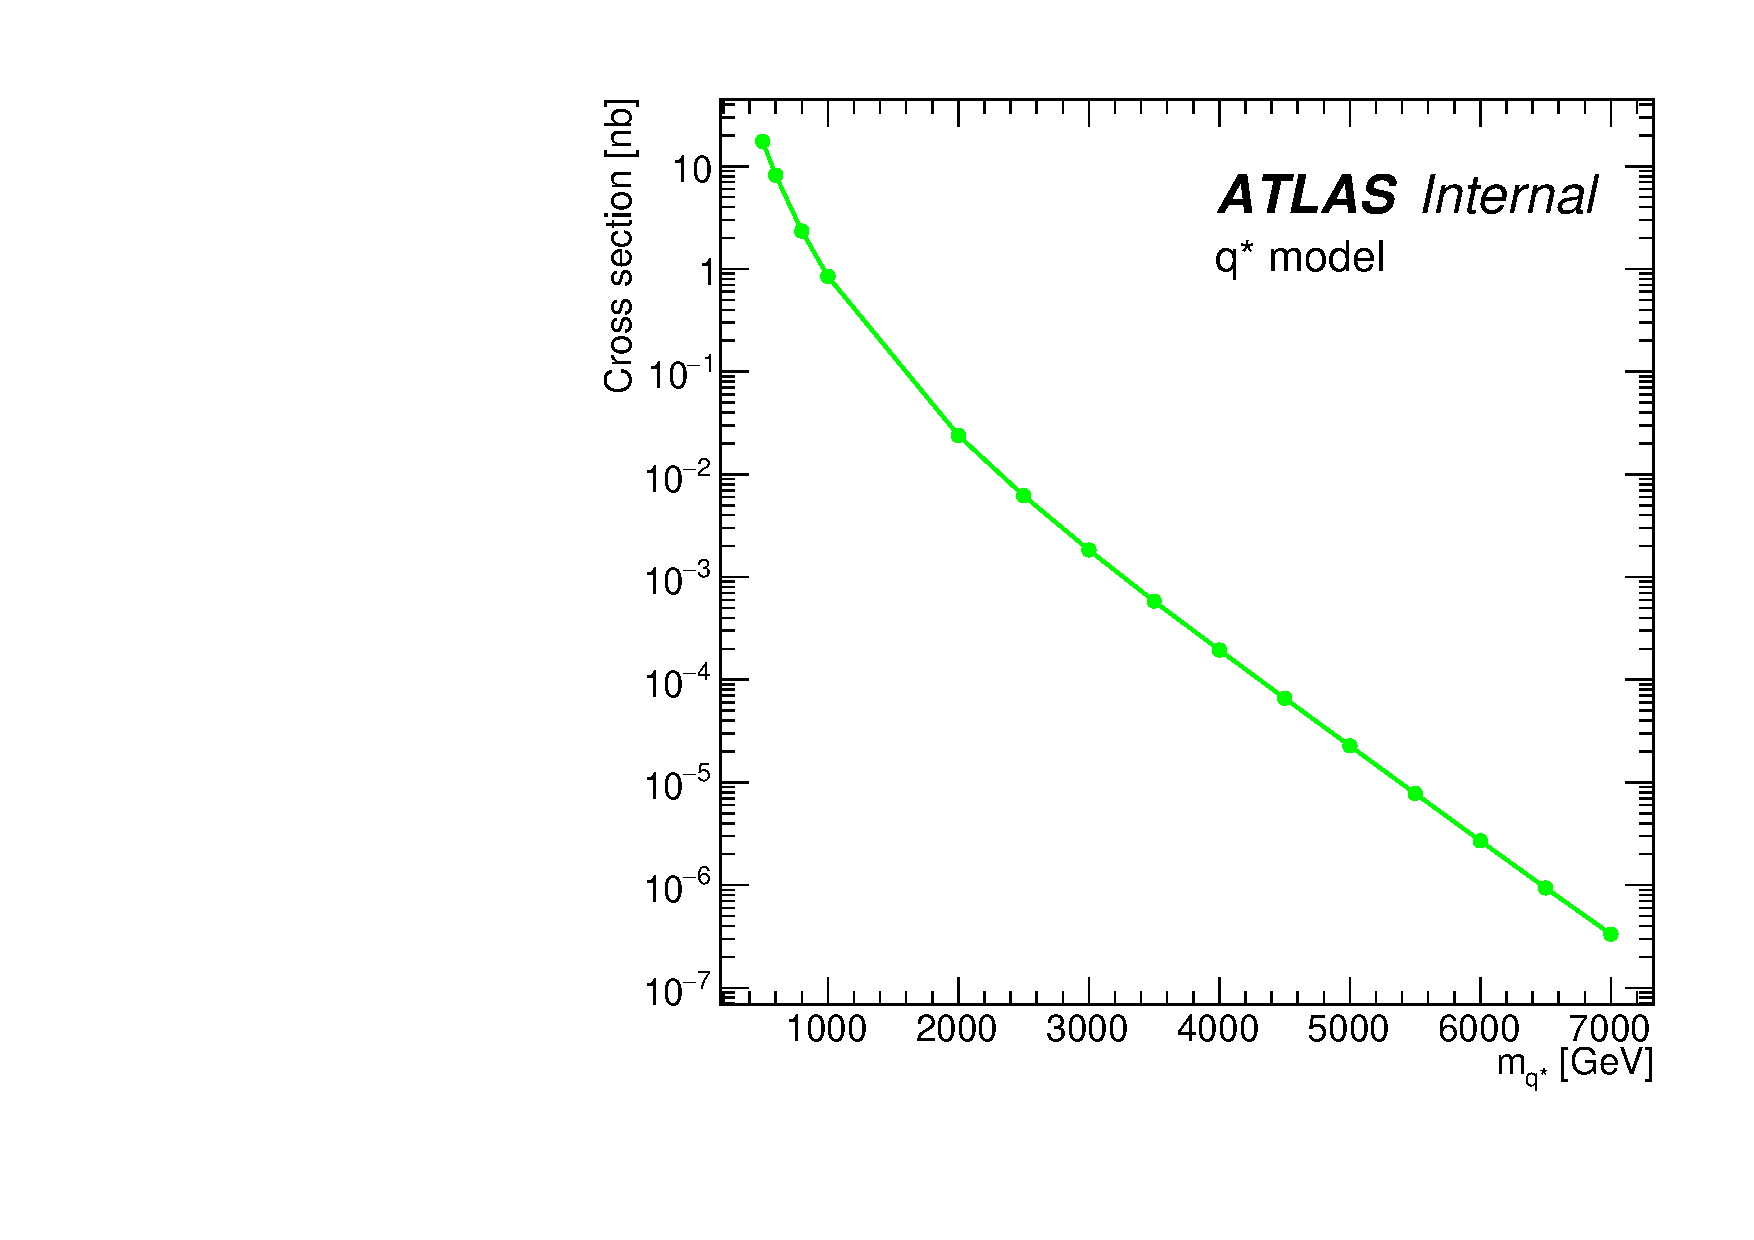
\includegraphics[width=0.9\textwidth]{figuresDijet/03-BenchmarkSignals/Xsec_Qstar.pdf}
   \caption{}
   \label{fig:QStar}
  \end{subfigure}
  \begin{subfigure}{.5\textwidth}
  \centering
   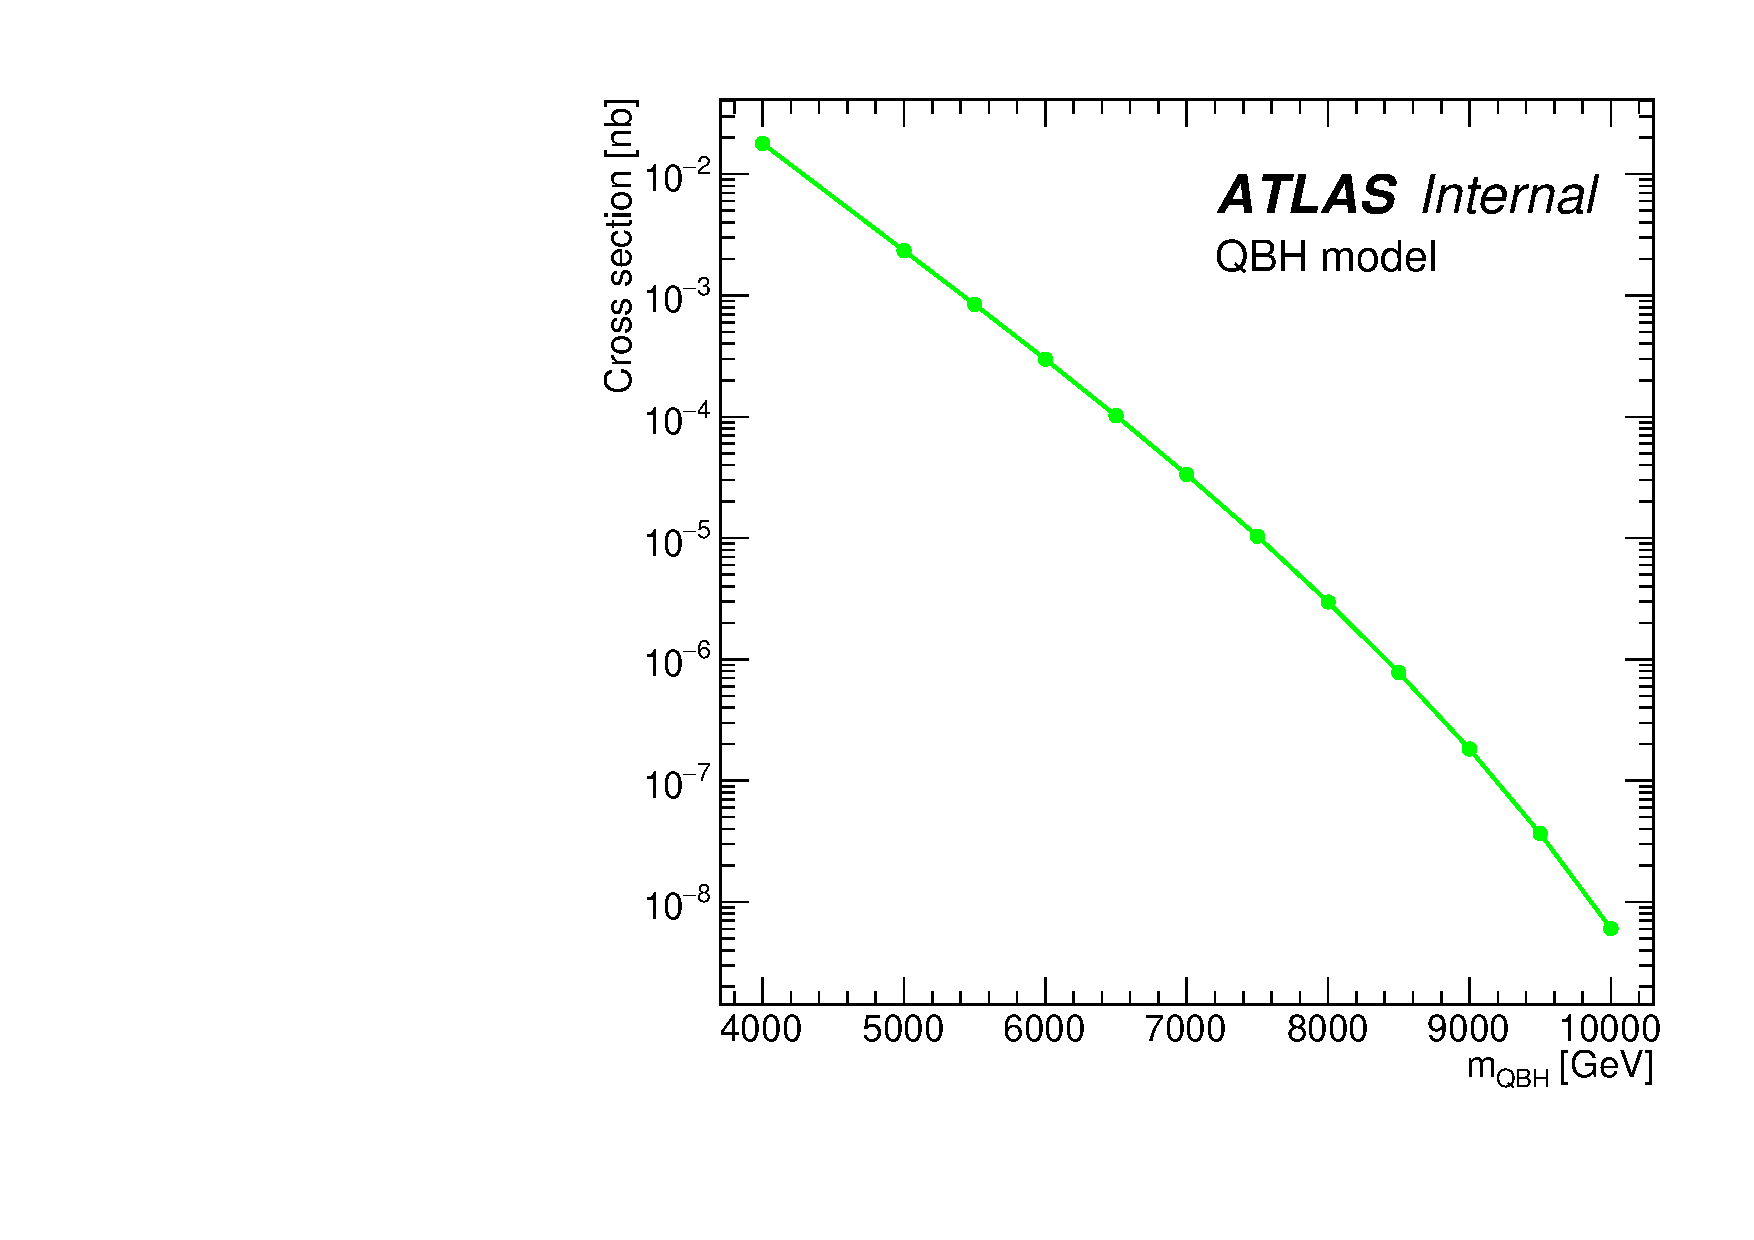
\includegraphics[width=0.9\textwidth]{figuresDijet/03-BenchmarkSignals/Xsec_QBH.pdf}
   \caption{}
   \label{fig:QBH}
  \end{subfigure}
\newline
  \begin{subfigure}{.5\textwidth}
  \centering
   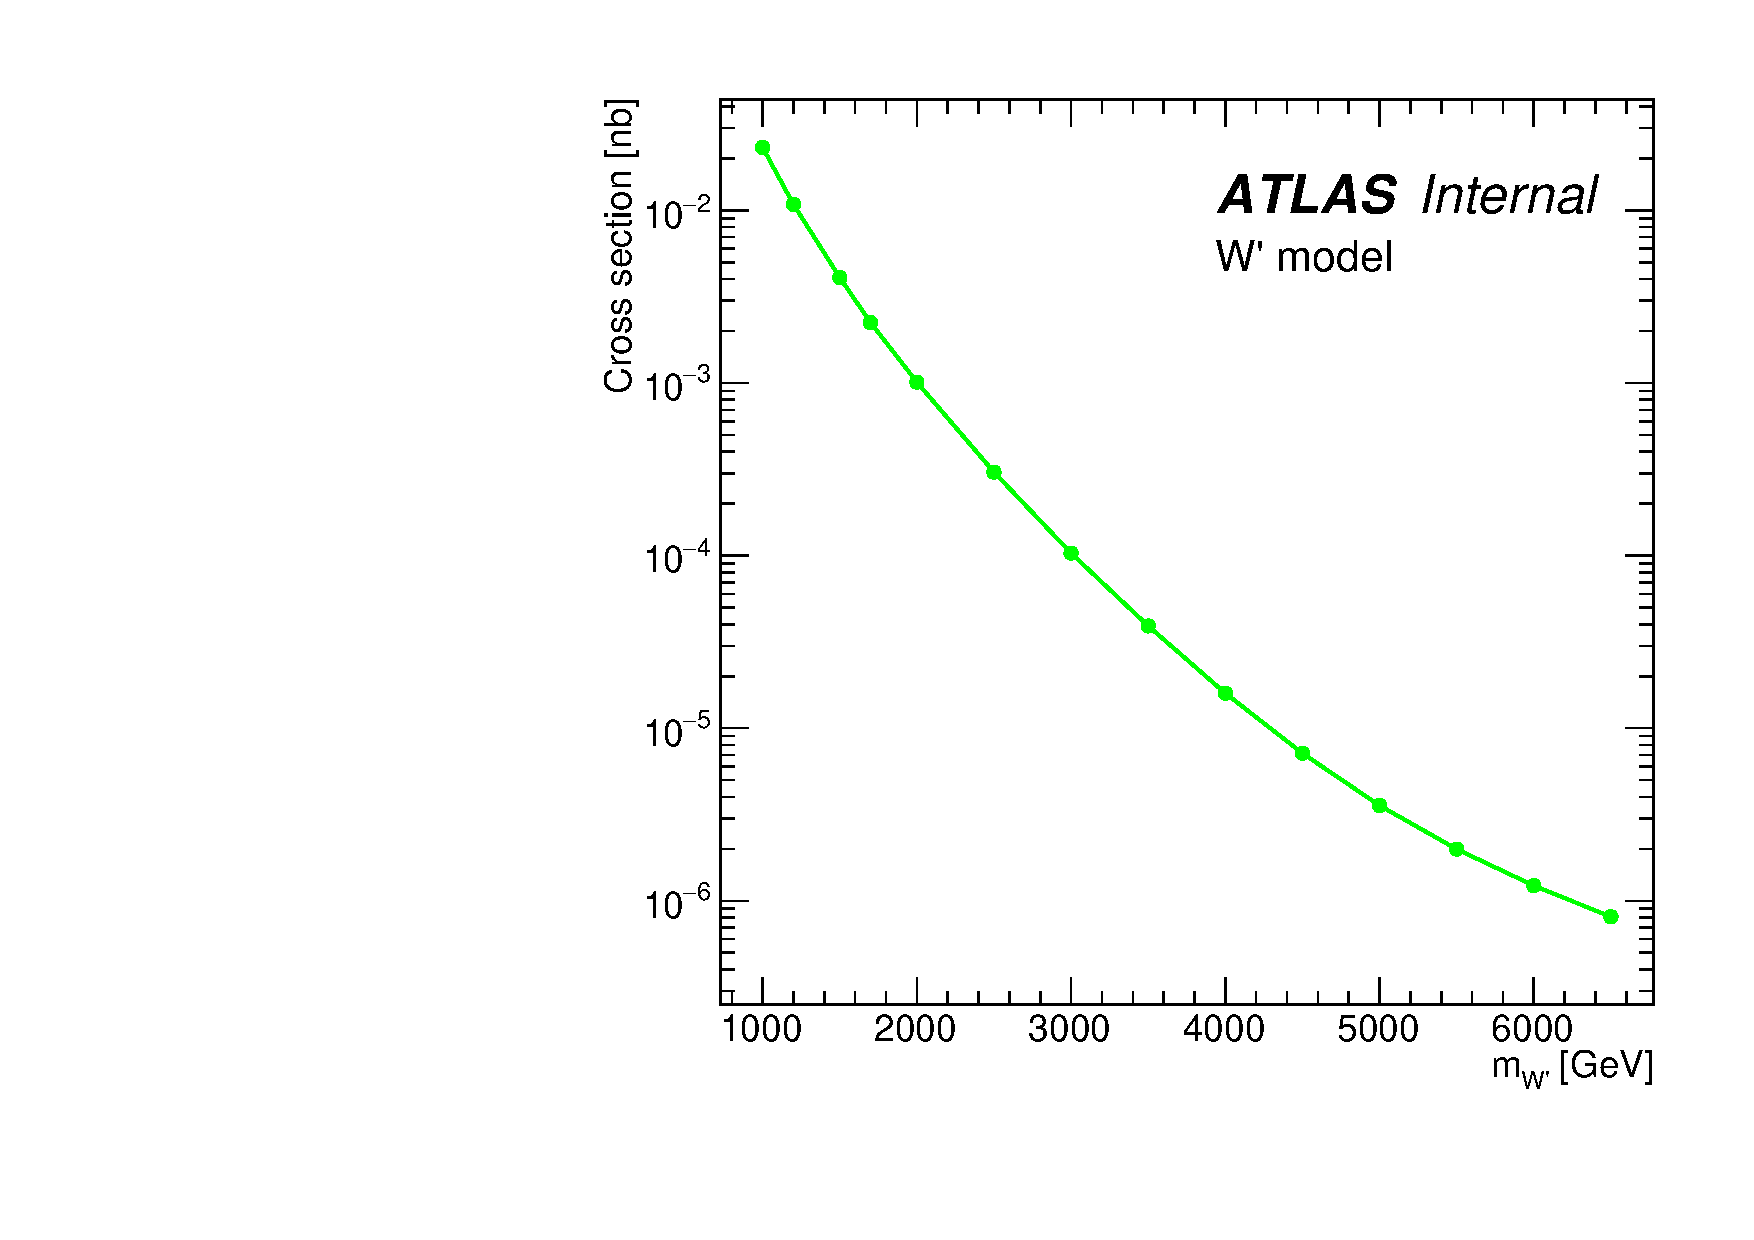
\includegraphics[width=0.9\textwidth]{figuresDijet/03-BenchmarkSignals/Xsec_Wprime.pdf}
   \caption{}
   \label{fig:WPrime}
  \end{subfigure}
  \begin{subfigure}{.5\textwidth}
  \centering
   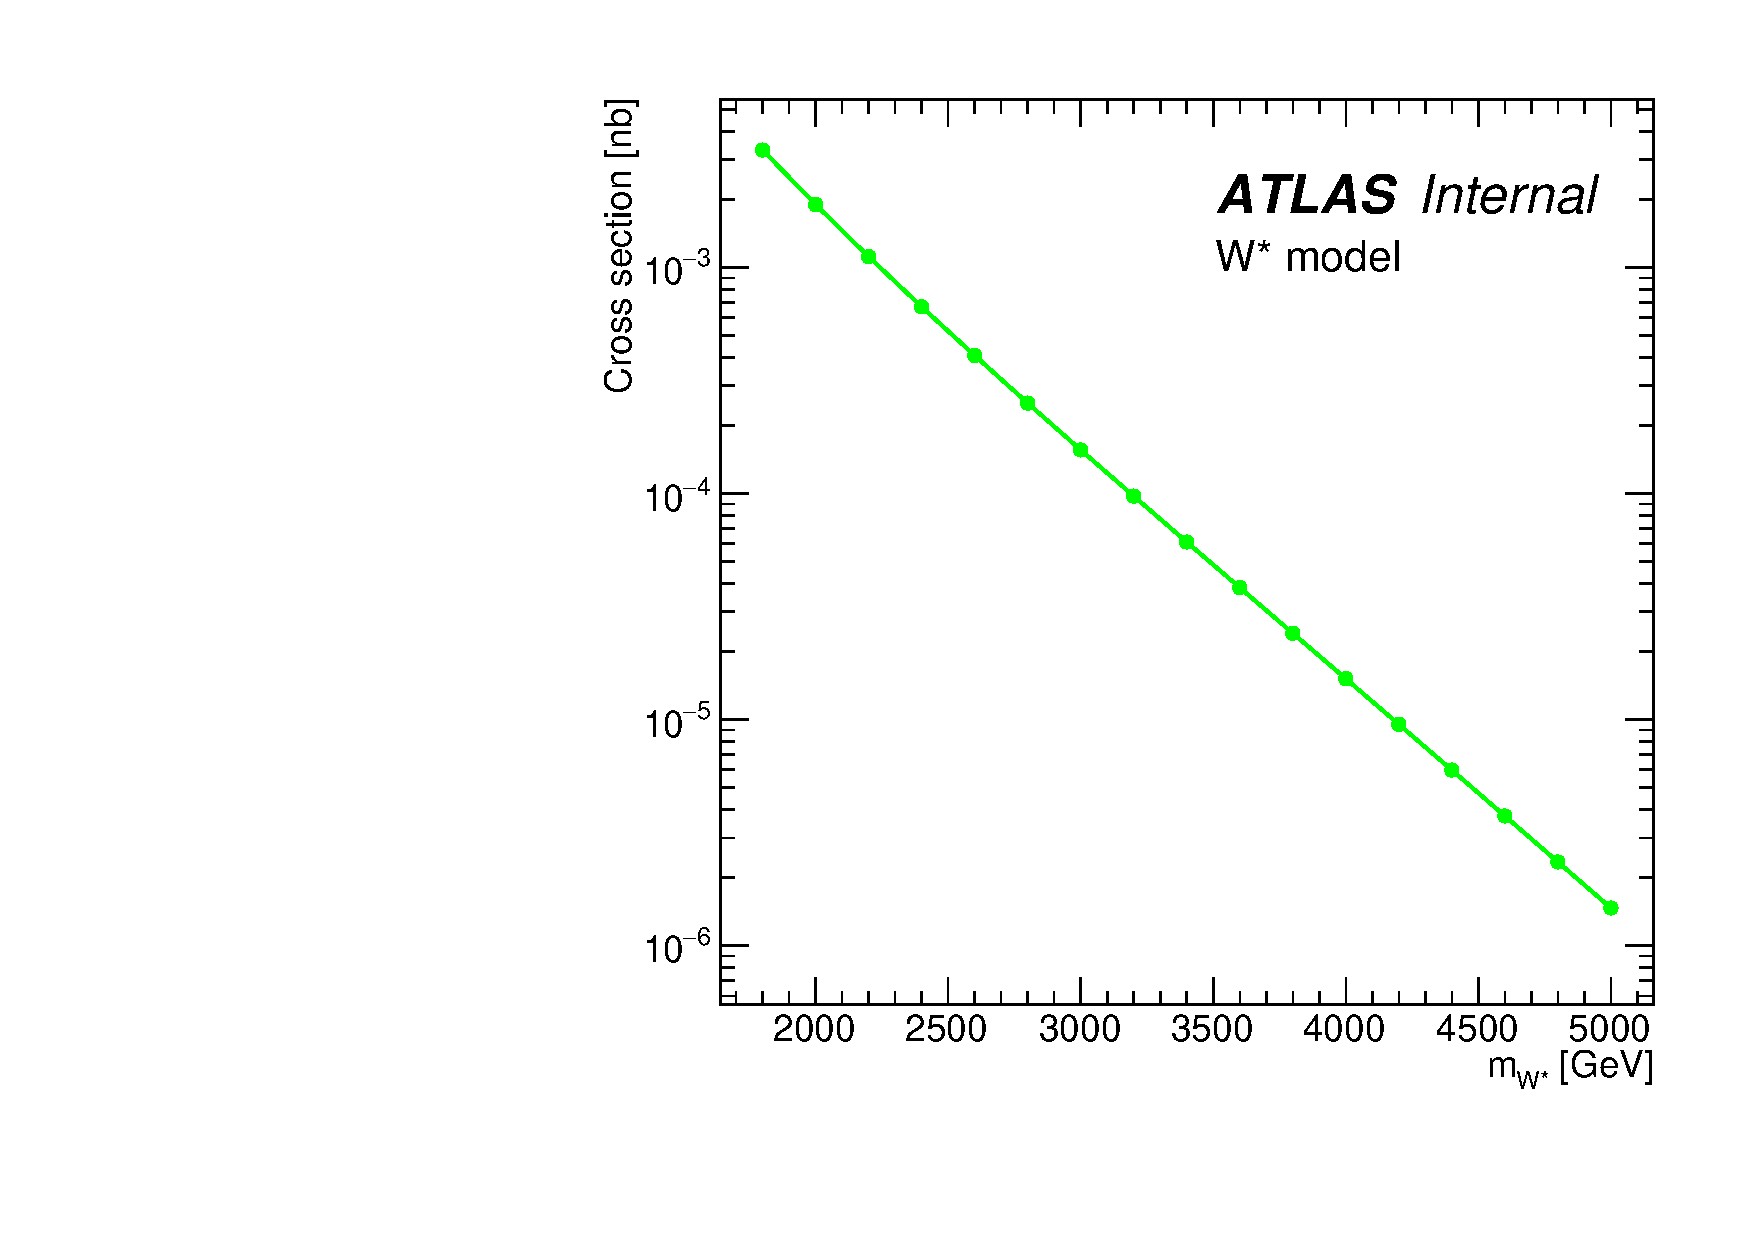
\includegraphics[width=0.9\textwidth]{figuresDijet/03-BenchmarkSignals/Xsec_Wstar.pdf}
   \caption{}
   \label{fig:WStar}
  \end{subfigure}
  \caption{
在全包含信号区中基准信号的散射截面随着信号质量的关系:
(a) 不同$q^*$质量所对应的散射截面;(b) 各个不同的$M_{D}$所对应的散射截面;(c) 不同$W\prime$质量所对应的散射截面;(d) 不同$W^*$玻色子质量所对应的散射截面。
  }
  \label{fig:Data1}
\end{figure} 



与标准模型中夸克具有轴矢流(V-A)耦合的非轻子耦合态$Z\prime$模型包含有一个狄拉克费米子暗物质(DM)候选粒子~\cite{DM3}。由DM $Z\prime$衰变到$q\bar{q}$的事例是用MadGraph5\_aMC@NLO 2.4.3~\cite{Alwall:2014hca}模拟的,其中$q=(u,d,s,c,b)$,并且此处暗物质质量被固定在$10TeV$,其与暗物质的耦合常数($g_\chi$)被设置为$1.5$。被模拟的媒介子DM $Z\prime$的质量范围为$1TeV$到$7TeV$,其与标准模型中夸克的耦合常数$g_{SM}$变化范围为$0.1$到$0.5$,图示~\ref{fig:Data2}~是在$g_{SM}$取不同值情况不同DM $Z\prime$质量所对应的散射截面。
这里,DM $Z\prime$并不会衰变到暗物质候选粒子,因此,dijet共振态信号仅仅取决于它的质量和其与标准模型中夸克的耦合常数。耦合常数$g_{SM}=0.5$所对应的DM $Z\prime$衰变宽度为共振态质量的$12\%$,达到了这个分析最大灵敏度。

\begin{figure}[thbp]
  \centering
  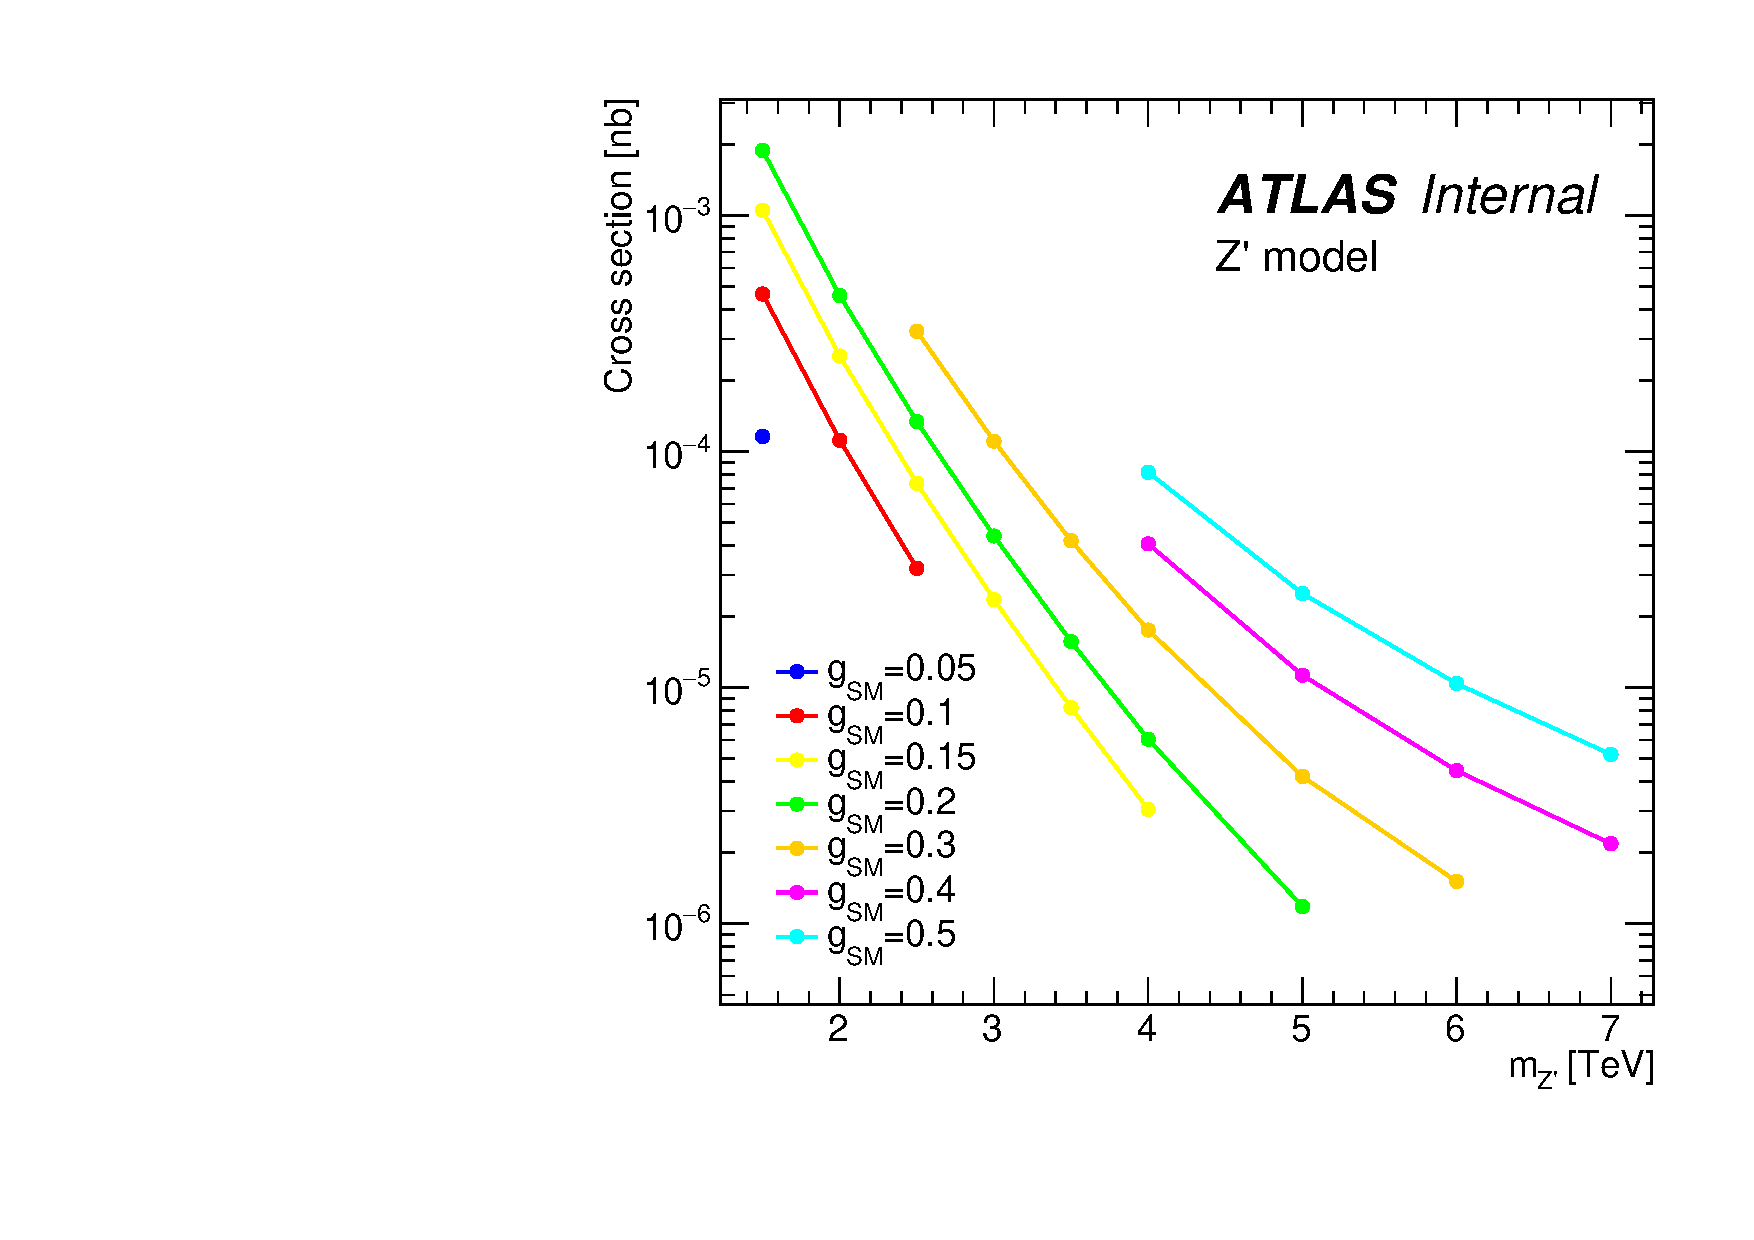
\includegraphics[width=0.75\textwidth]{figuresDijet/03-BenchmarkSignals/Xsec_Zprime.pdf}
  \caption{  当$g_{SM}$取不同值时不同DM $Z\prime$质量所对应的散射截面。}
  \label{fig:Data2}
\end{figure}

对于区分末态jet味信息的信号区1b和2b,DM $Z\prime$衰变到$b\bar{b}$末态的事例是使用同样的产生子模拟的,其衰变分支比$\mathcal{B}(DM Z\prime \to b\bar{b})$达到了$18.9\%$。
我们还模拟了激发态$b$夸克($b^*$)信号模型的事例,信号质量区间和产生子设置都和全末态模拟的情形类似。并且这里我们模拟了全部的衰变道,包括主要的衰变道$bg$,所占的分支比达到了$85\%$,和其他几个次要的衰变道$b\gamma$、$bZ$和$tW$。

连续标准模型中$Z\prime$玻色子~\cite{zprime1}可以与标准模型中费米子耦合,并且与标准模型中$Z$玻色子有着相同的耦合常数,因此其$b$夸克衰变分支比$\mathcal{B}(SSM Z\prime \to b\bar{b})$有$13.8\%$,其衰变宽度为大约是其质量的$3\%$。
这里SSM $Z\prime$到$b\bar{b}$衰变道的事例是用\textsc{Pythia 8.186}产生,精确到领头阶,随后散射截面被修正到次领头阶~\cite{Alwall:2014hca}。

在Randall-Sundrum额外维模型~\cite{RS1,RS2}中,自旋为2的Kaluza-Klein(KK)引力子(Graviton)会优先衰变到夸克和胶子。此处,引力子信号模型是用\textsc{Pythia 8.212}产生的,并且假定曲率参数(the curvature parameter)$k/\overline{M}_\text{PL}=0.2$,其中$\overline{M}_\text{PL}$是四维简化的普朗克刻度(Plank scale)。这里仅模拟了衰变道KK $G \rightarrow b\bar{b}$的事例,所模拟的KK引力子的质量为$1.25TeV$到$7TeV$。

图示~\ref{fig:Data3}~总结了区分末态jet味信息的信号区中基准信号的散射截面乘以分支比与信号质量的关系。

\begin{figure}[thbp]
  \centering
  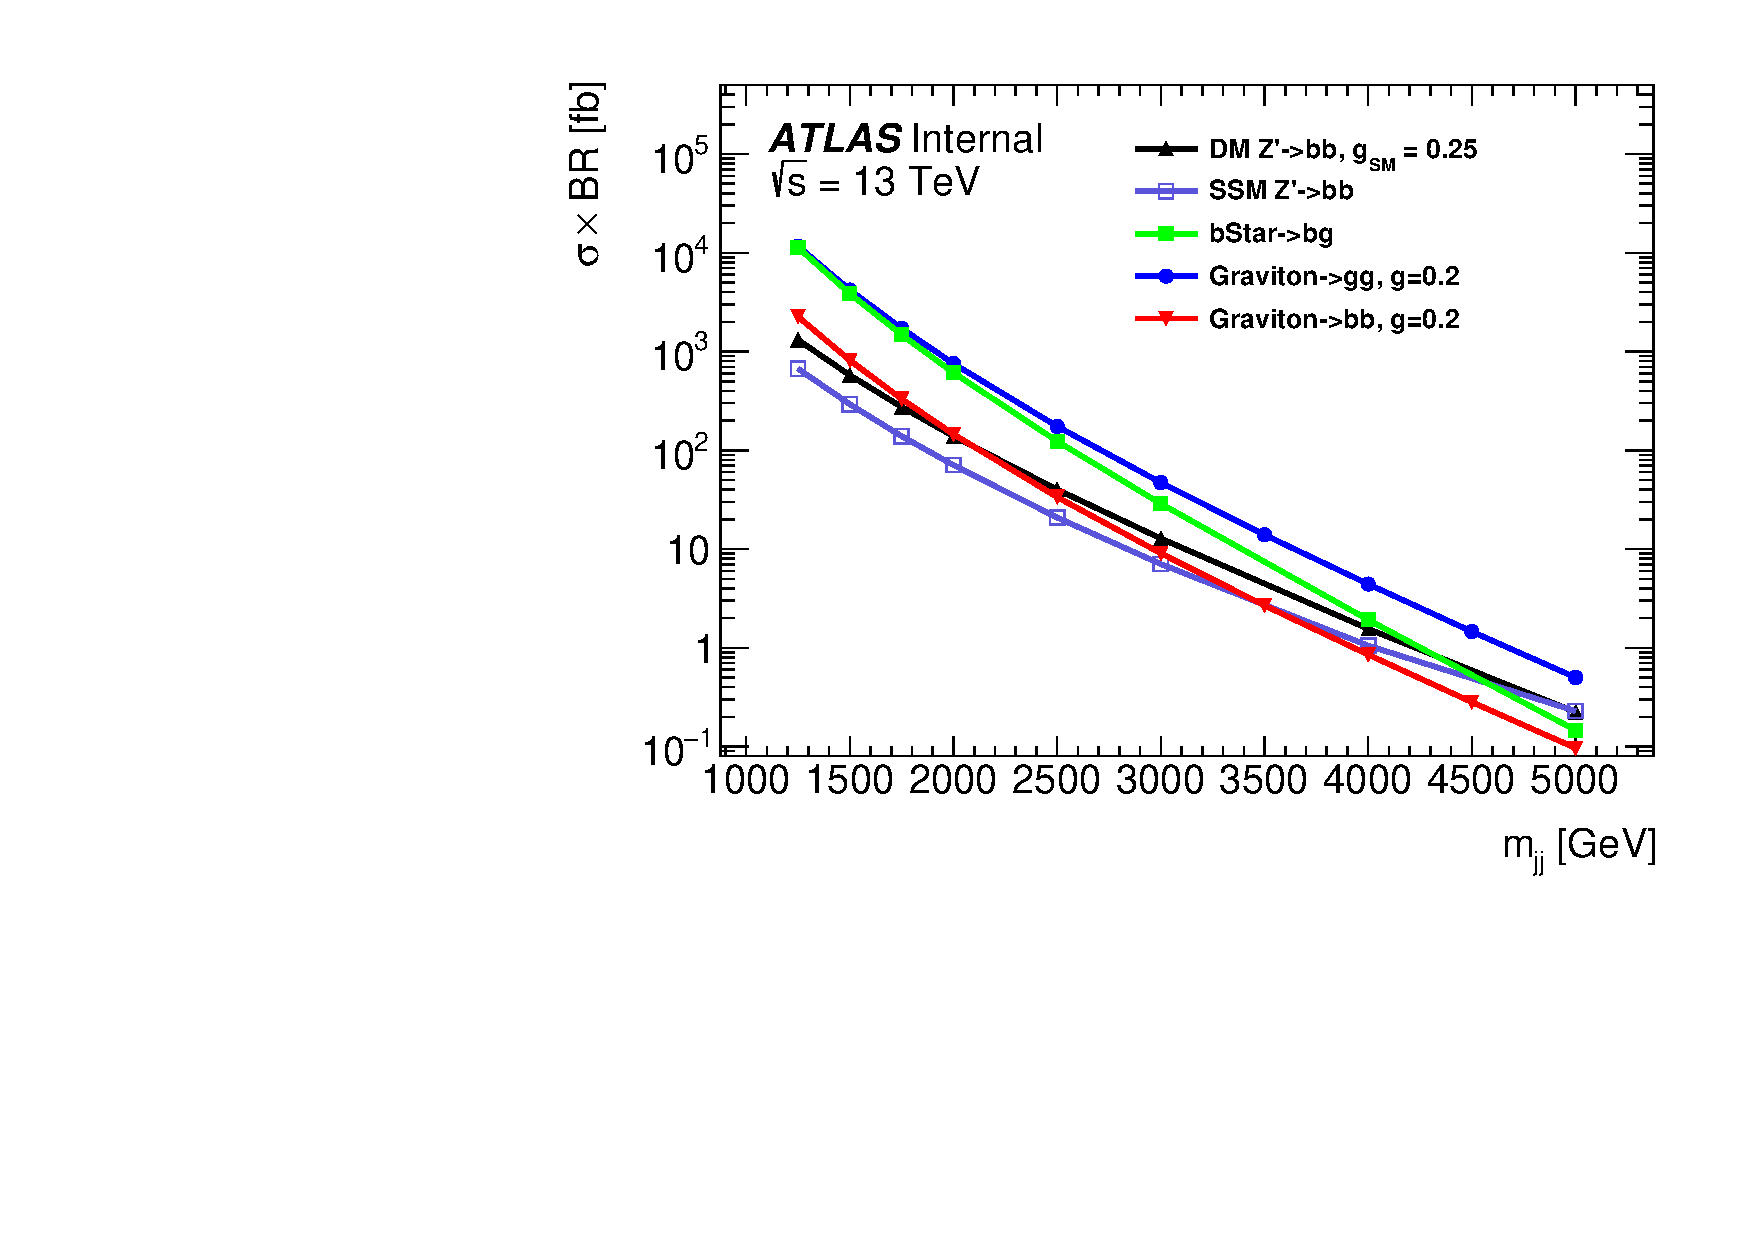
\includegraphics[width=0.75\textwidth]{figuresDijet/03-BenchmarkSignals/taggedSignal_xs.pdf}
  \caption{ 区分末态jet味信息的信号区1b和2b中基准信号的散射截面乘以分支比与信号质量的关系。 }
  \label{fig:Data3}
\end{figure}

由MC产生的QCD过程的事例随后会通过用Geant 4~\cite{Agostinelli:2002hh}模拟的ATLAS探测器,由此来模拟事例在探测器中的行为。而由MC产生的信号事例随后会通过一个仅依赖于参数化的量能器响应的快模拟过程~\cite{ATL-PHYS-PUB-2010-013}。
其中b强子和c强子的衰变过程由\textsc{EvtGen 1.2.0}~\cite{Lange:2001uf}来实现。
为了将堆积事例考虑进去,我们用\textsc{Pythia 8.186}模拟了一系列非弹性的质子-质子相互作用,这里使用了部分子分布函数集NNPDF23LO~\cite{Martin:2009iq}和校准参数集ATLAS A3~\cite{ATL-PHYS-PUB-2016-017},这些事例随后被叠加在那些硬散射(hard-scattering)事例上面。
为了使模拟和数据中每个束流的平均碰撞数目的分布吻合,所有的模拟事例都被重新赋予权重因子。



\section{事例重建和筛选}
\label{sec:DijetSelection}

%实验数据来自于LHC上ATLAS探测器从2015年到2018年收集的质心系能量为$\sqrt{s}=13TeV$的质子质子对撞产生的数据。在要求探测器系统正常运转并收集到高质量数据的条件下,此期间数据总的积分亮度达到了$139fb^{-1}$。
%使用LUCID-2探测器~\cite{LUCID2}作为主要的亮度测量机器,我们得到的总的积分亮度的不确定度为$1.7\%$~\cite{ATLAS-CONF-2019-021}。

%事例筛选是通过基于软件的高级触发器来实现的,要求事例中至少有一个jet的横动量大于$420GeV$,所用到的触发器是未预分频的单jet最小横动量触发器~\cite{}。

\subsection{事例重建}
\label{sec:DijetSelection1}
从径迹到jet的重建在第~\ref{sec:JET}~小节有简要介绍,这个分析所用的jet类型都为SR-jet。
碰撞顶点的重建条件是和顶点关联的径迹中至少有两条满足$p_{T}>0.5GeV$,而主顶点的选择标准是和顶点关联的所有径迹的横动量平方和$\sum p^2_{T}$最大。
在事例重建过程中,那些能量沉积显著高于量能器噪声水平的量能器单元会根据其连续性形成拓扑集群~\cite{PERF-2014-07},然后通过距离参数R=0.4的$anti$-$k_{t}$算法~\cite{Cacciari:2008gp, Fastjet}会聚成SR-jet,最后通过jet校准~\cite{PERF-2016-04}对jet的能量和方向进行修正。
并且我们还排除了那些事例中$p_{T}>150GeV$的jet可能来自于突发噪声、束流诱发的背景或者宇宙射线的事例~\cite{ATLAS-CONF-2015-029}。
事例筛选是通过基于软件的高级触发器来实现的,要求事例中至少有一个jet的横动量大于420GeV,所用到的触发器是未预分频的single-jet最小横动量触发器~\cite{ATLASRTS}。


\subsection{事例筛选}
\label{sec:DijetSelection2}
事例中至少要包含两个横动量都大于$150GeV$的jet,而且要求两个横动量最高的jet即两个领头阶jet之间的方位角$|\Delta \phi(jj)|$大于$1.0$。
为了最大程度上提高对各个信号模型的灵敏度,
信号区(Signal regions)的按事例中b-jet标定的情况被分成了三个信号区,分析所使用的b-jet标定技术将在下一节介绍,
包括不区分末态jet味信息的全包含信号区,以及区分末态jet味信息的信号区:末态两个横动量($p_{T}$)最高的jet中一个被标定为b-jet的1b信号区和其中的两个jet都被标定为b-jet的2b信号区。
分析所使用的b-jet标定技术将在下一节介绍。

对于区分末态jet味信息的两个信号区,两个领头阶jets的赝快度之差的绝对值满足$|\eta|<2.0$,这个筛选条件是为了减少高赝快度区间的系统误差。
为了减小主要来自于QCD过程的本底贡献,我们引入了一个针对于两个领头阶jets的快度之差的二分之一$y^*=|y_1-y_2|/2$的筛选条件,其中$y_1$和$y_2$分别为领头阶jet和次领头阶jet的快度。
信号事例是通过s散射道(s-channel)过程产生的,事例所对应的$y^*$都偏小,而大部分本底事例都是来自于对应的$y^*$都偏大的QCD过程中的t散射道过程。
针对不同的信号区和信号模型,我们优化了对于$|y^*|$的事例筛选条件。

在全包含信号区,除了$W^*$,对于其他所考虑到的信号,我们要求$|y^*|<0.6$ ,
由于$W^*$更加青睐于$|y^*|$较大的衰变模式,
如图~\ref{fig:Selection1}~所示是$W^*$信号和QCD中两个领头阶jet的快度之差$|y_1-y_2|$分布的对比和信号显著性随着$|y_1-y_2|$筛选值的变化关系,
可以看到$|y_1-y_2|$在2左右显著性最高,因此对于$W^*$我们要求$|y^*|<1.2$。

\begin{figure}[htbp]
  \begin{subfigure}{.5\textwidth}
  \centering
   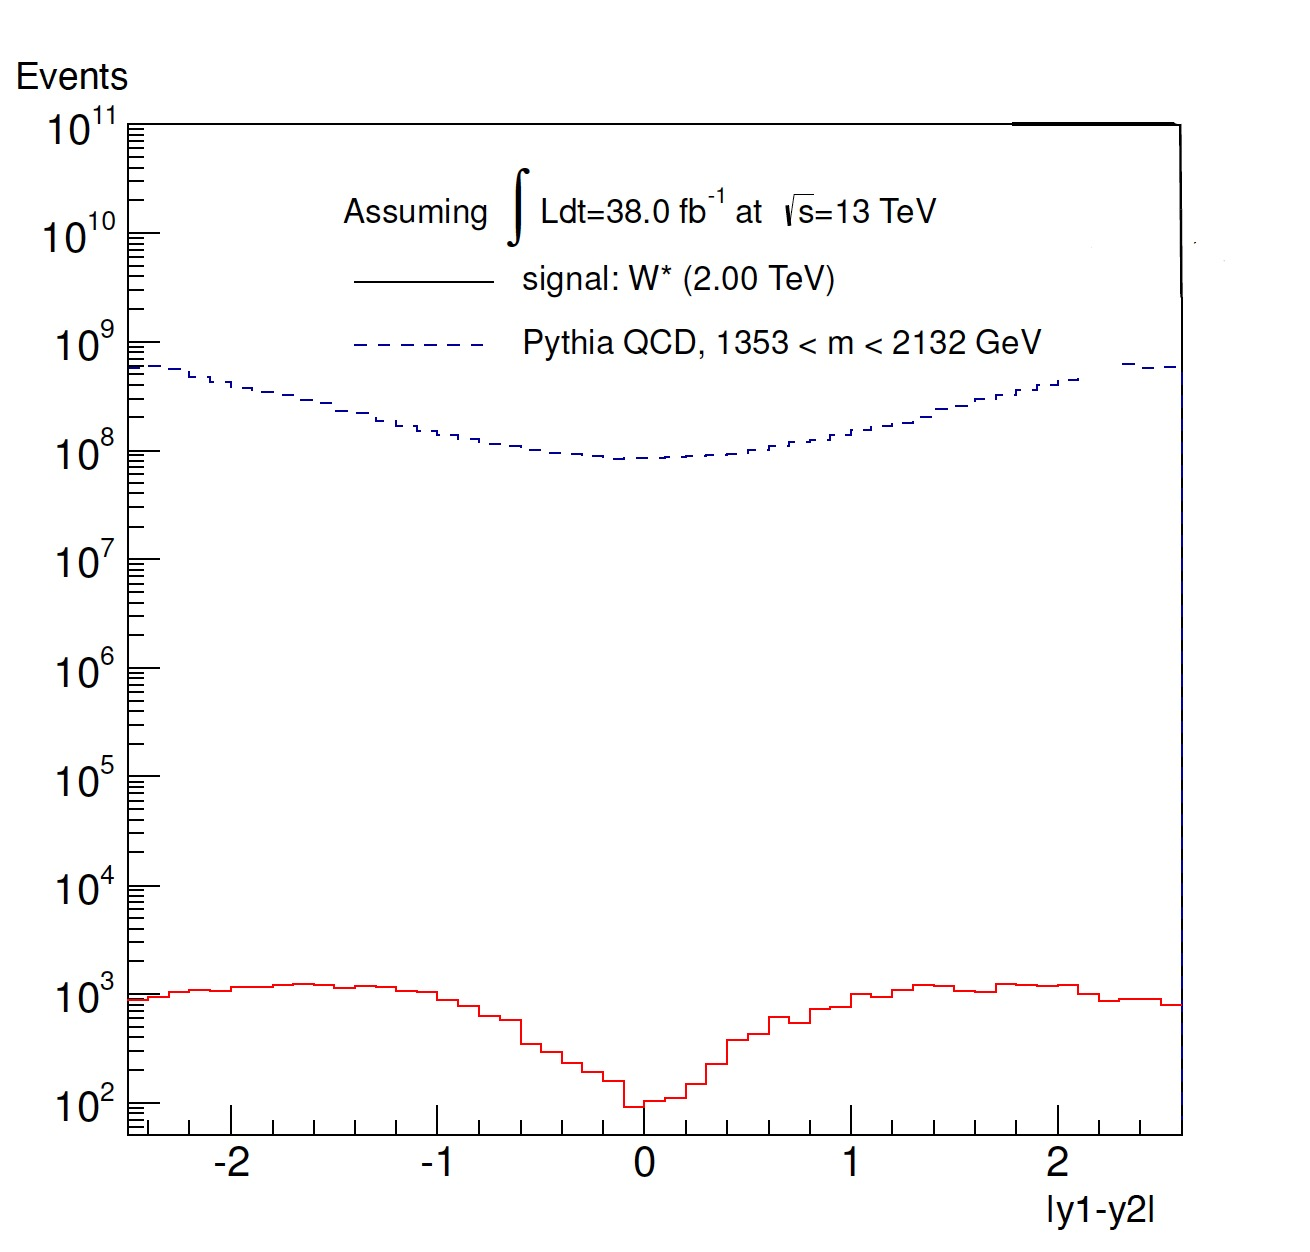
\includegraphics[width=0.9\textwidth]{figuresDijet/03-BenchmarkSignals/DeltaY.jpg}
   \caption{$|y_1-y_2|$分布对比}
   \label{fig:WSY1}
  \end{subfigure}
  \begin{subfigure}{.5\textwidth}
  \centering
   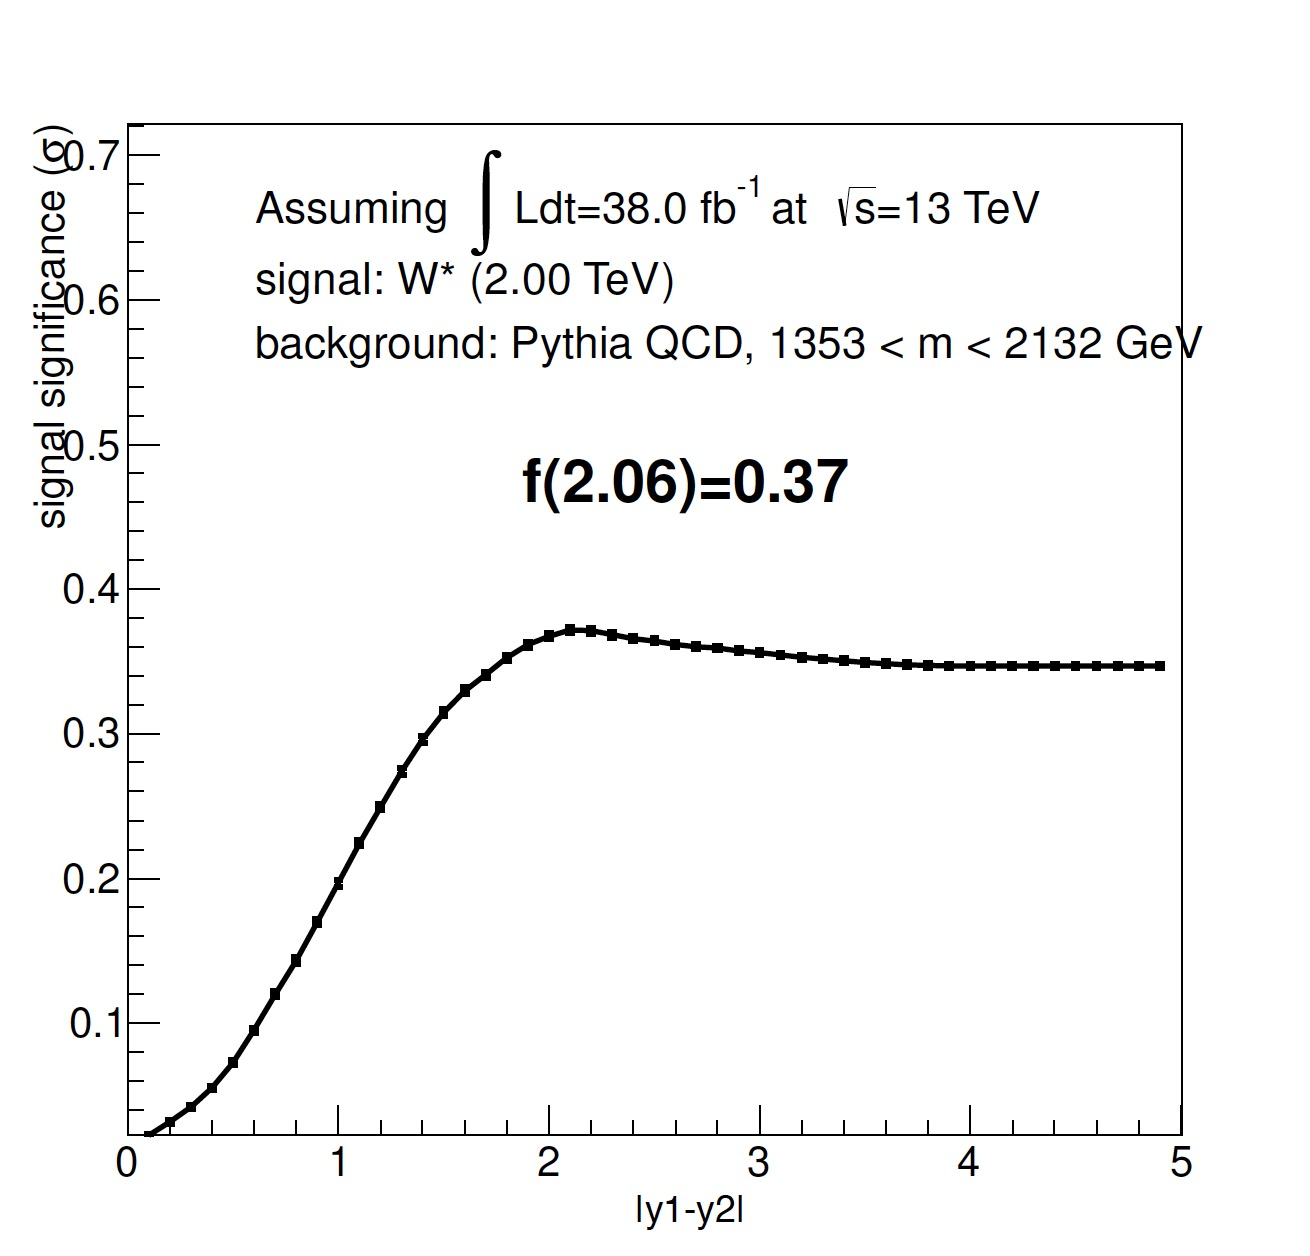
\includegraphics[width=0.9\textwidth]{figuresDijet/03-BenchmarkSignals/Significance.jpg}
   \caption{显著性随着$|y_1-y_2|$的变化}
   \label{fig:WSY2}
  \end{subfigure}
  \caption{$W^*$信号和QCD中两个领头阶jet的快度之差$|y_1-y_2|$分布的对比(左图)和信号显著性随着$|y_1-y_2|$筛选值的变化关系(右图)。}
  \label{fig:Selection1}
\end{figure} 

在$1b$和$2b$信号区,我们要求$|y^*|<0.8$,这是根据所选择的b-jet标定技术基于最高灵敏度对$y^*$筛选条件进行优化得到的,在下一节将会介绍。
为了保证完全有效的没有运动学偏差的筛选条件,我们对$m_{jj}$设置了一个下限,
它取决于所选择的single-jet触发器的开启效率和对于$|y^*|$的筛选条件。在$m_{jj}$和$|y^*|$筛选条件的范围内,领头阶jet的横动量高于single-jet触发器的阈值。
表~\ref{tab:selection}~总结了这个分析所使用的筛选条件和所寻找的相应的信号模型。

\begin{table}[htbp]
  \caption{ 这个分析所使用的筛选条件和所寻找的相应的信号模型的总结表,筛选条件仅包括事例中两个横动量最高的jet。}
  %Summary of the event selection requirements and benchmark signals being tested in each analysis category. Only the two jets with highest \pt enter in the event selection. The exact values of the \mjj lower bounds also depend on the jet energy resolution uncertainty.
  \centering
  \begin{tabular}{l|c|c|c|c}
    \hline\hline
    Category & \multicolumn{2}{c|}{Inclusive} & $1b$ & $2b$ \\\hline
    Jet $p_{T}$ & \multicolumn{4}{c}{$>150 GeV$} \\\hline
    Jet $\phi$ & \multicolumn{4}{c}{$|\Delta \phi(jj)|>1.0$} \\\hline
    %Jet $\eta$ & \multicolumn{2}{c|}{$<5.0 $} &  \multicolumn{2}{c}{$<2.0 $} \\\hline
    Jet $|\eta|$& \multicolumn{2}{c|}{-} &  \multicolumn{2}{c}{$<2.0 $} \\\hline
    $|y^*|$ & $<0.6$ &  $<1.2$ &  \multicolumn{2}{c}{$<0.8$} \\\hline
    $m_{jj}$ & $>1100 GeV$ & $>1717 GeV$ & \multicolumn{2}{c}{$>1133 GeV$} \\\hline
    $b$-tagging & \multicolumn{2}{c|}{no requirement} & $\geqslant1$ $b$-tagged jet & 2 $b$-tagged jets \\\hline
    \multirow{5}{*}{Signal} & DM mediator $Z'$ & $W^*$ & $b^*$ & DM mediator $Z'$ ($b\overline{b}$) \\
    &$W'$ & & Generic Gaussian & SSM $Z'$ ($b\overline{b}$) \\
    & $q^*$  & &                 & graviton ($b\overline{b}$) \\
    & QBH    & &                 & Generic Gaussian \\
    & Generic Gaussian & &  & \\\hline
    \hline
  \end{tabular}
  \label{tab:selection}
\end{table}



\subsection{信号接收度}
\label{sec:DijetSelection3}

对于不同信号的接收度\footnote{接收度定义为通过筛选条件的信号事例数与总的信号事例数的比值。},
在全包含信号区,如图~\ref{fig:ACCP}~所示,展示了$q^*$、$QBH$、$W'$和$W^*$信号的接收度随着信号质量的变化,
对于所有被考虑到的质量点,$q^*$和$QBH$信号的接收度约为$55\%$,
$W'$信号的接收度取决于信号质量,并介于近似$20\%$和$45\%$之间,
对于$W^*$信号,随着信号质量从$2TeV$到$6TeV$变化,其接收度由$30\%$增加到$70\%$。
如图~\ref{fig:ACCPZ}~所示,展示了$Z'$信号的接收度随着信号质量的变化,
$Z'$信号的接收度同样取决于信号质量,并介于近似$20\%$和$45\%$之间。

\begin{figure}[htbp]
  \begin{subfigure}{.5\textwidth}
  \centering
   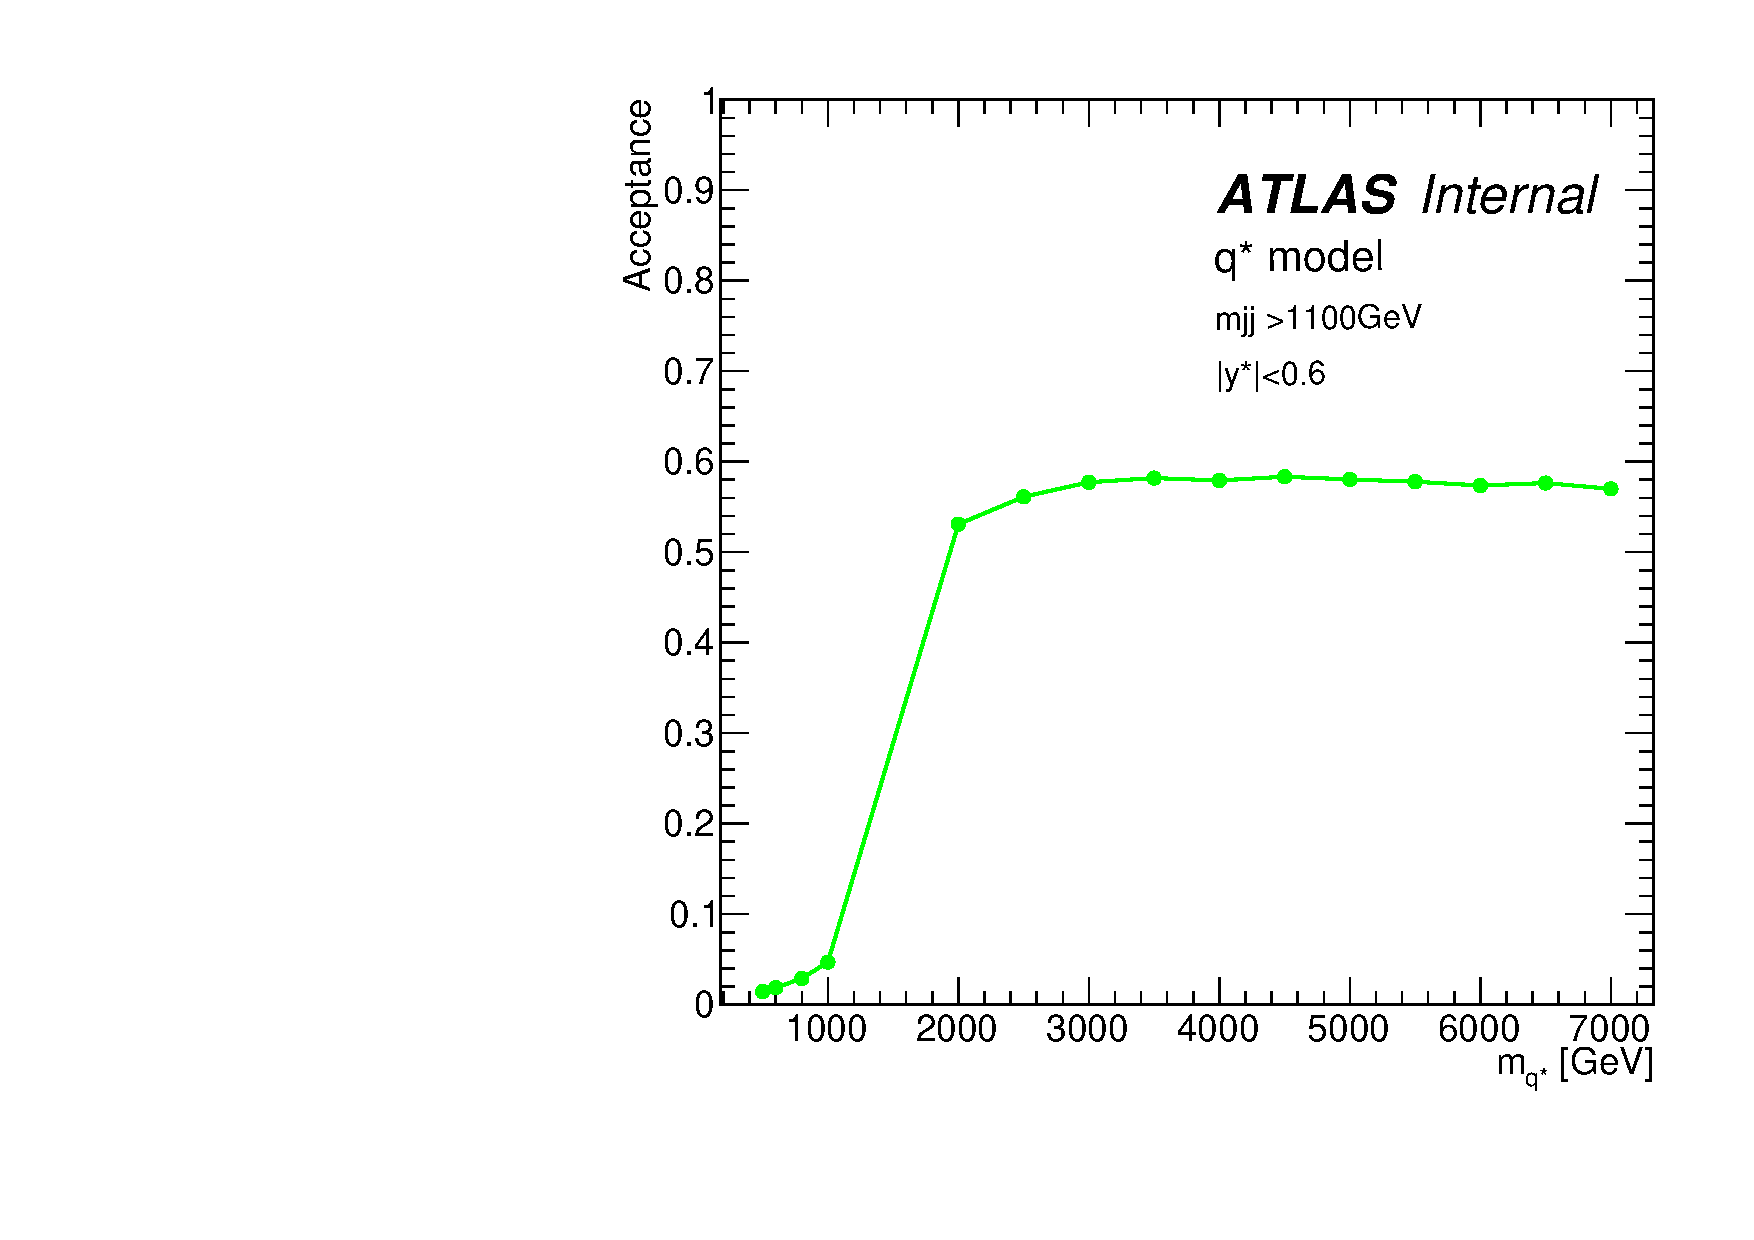
\includegraphics[width=0.9\textwidth]{figuresDijet/03-BenchmarkSignals/Acc_Qstar.pdf}
   \caption{}
   \label{fig:QStar1}
  \end{subfigure}
  \begin{subfigure}{.5\textwidth}
  \centering
   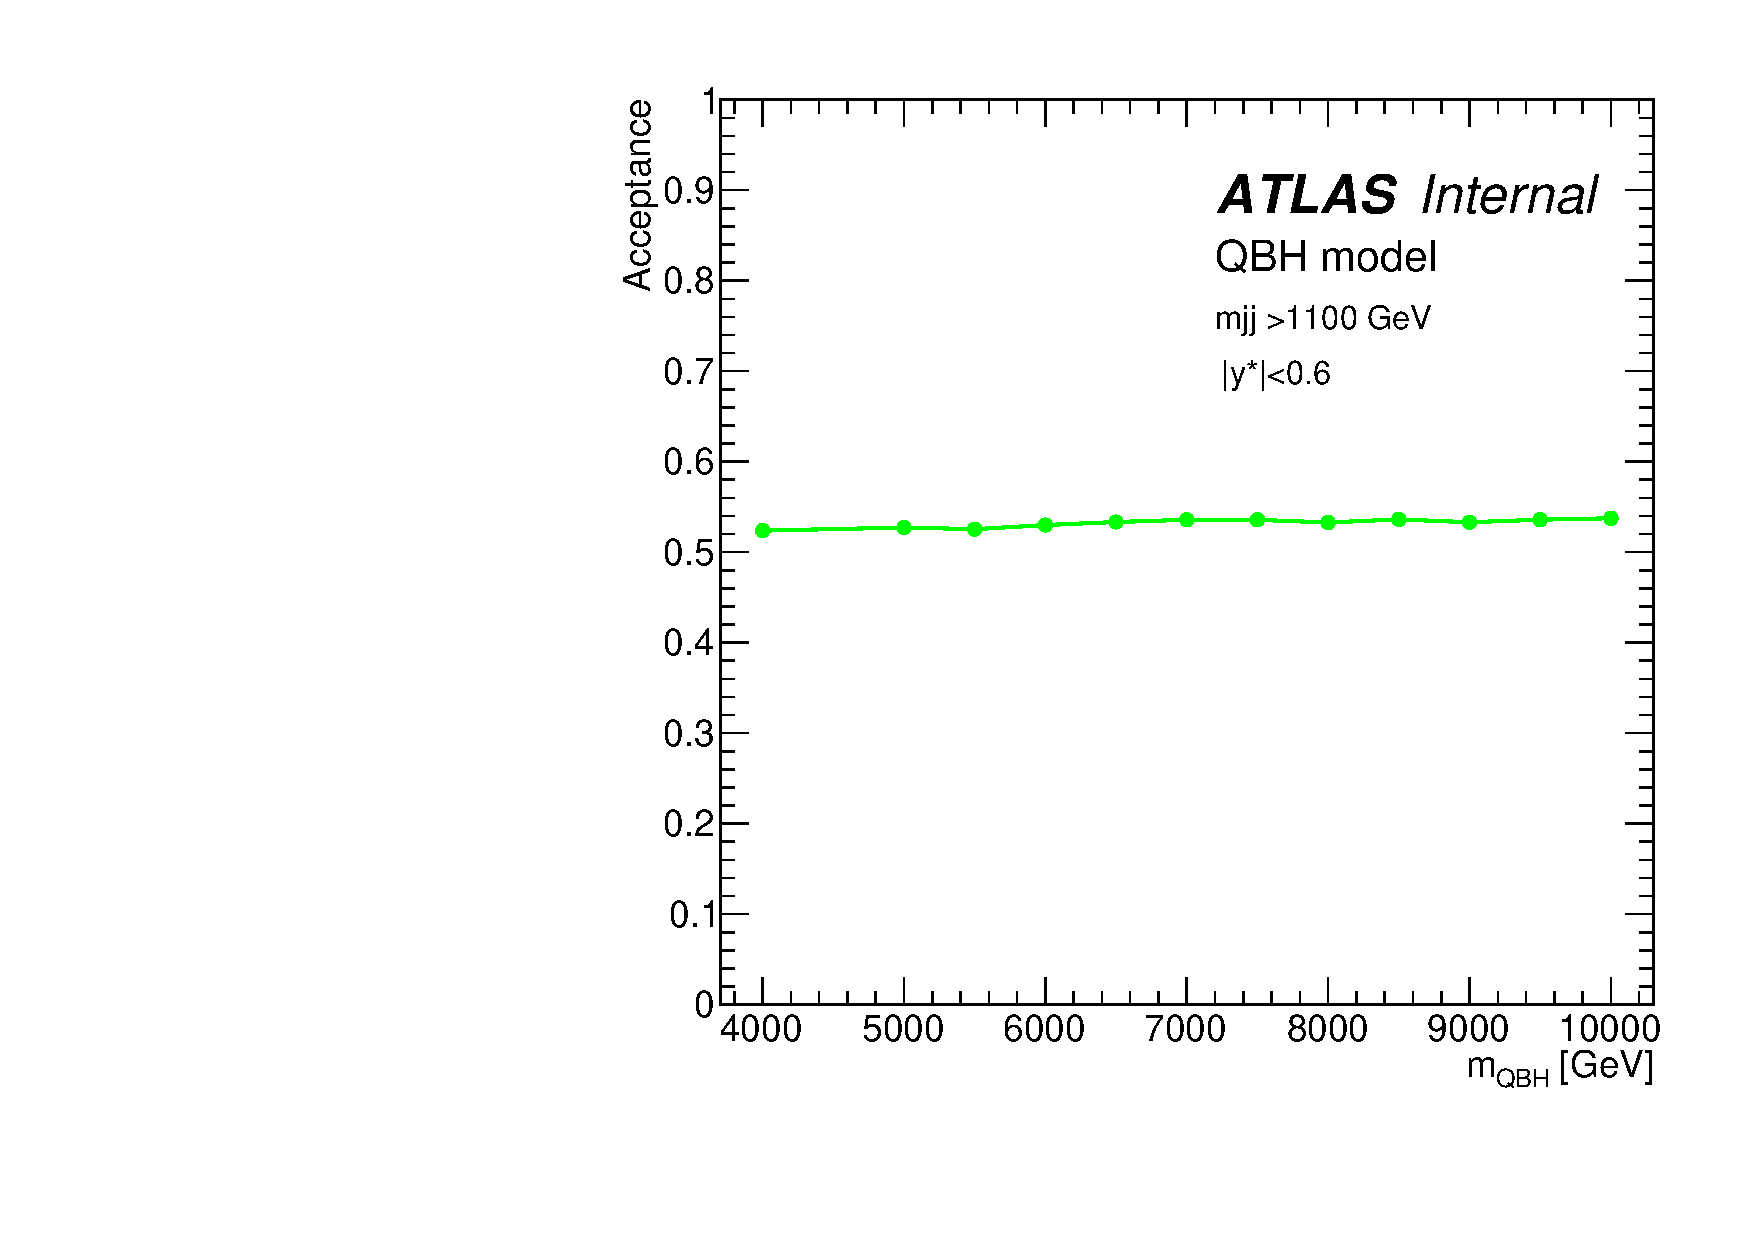
\includegraphics[width=0.9\textwidth]{figuresDijet/03-BenchmarkSignals/Acc_QBH.pdf}
   \caption{}
   \label{fig:QBH1}
  \end{subfigure}
\newline
  \begin{subfigure}{.5\textwidth}
  \centering
   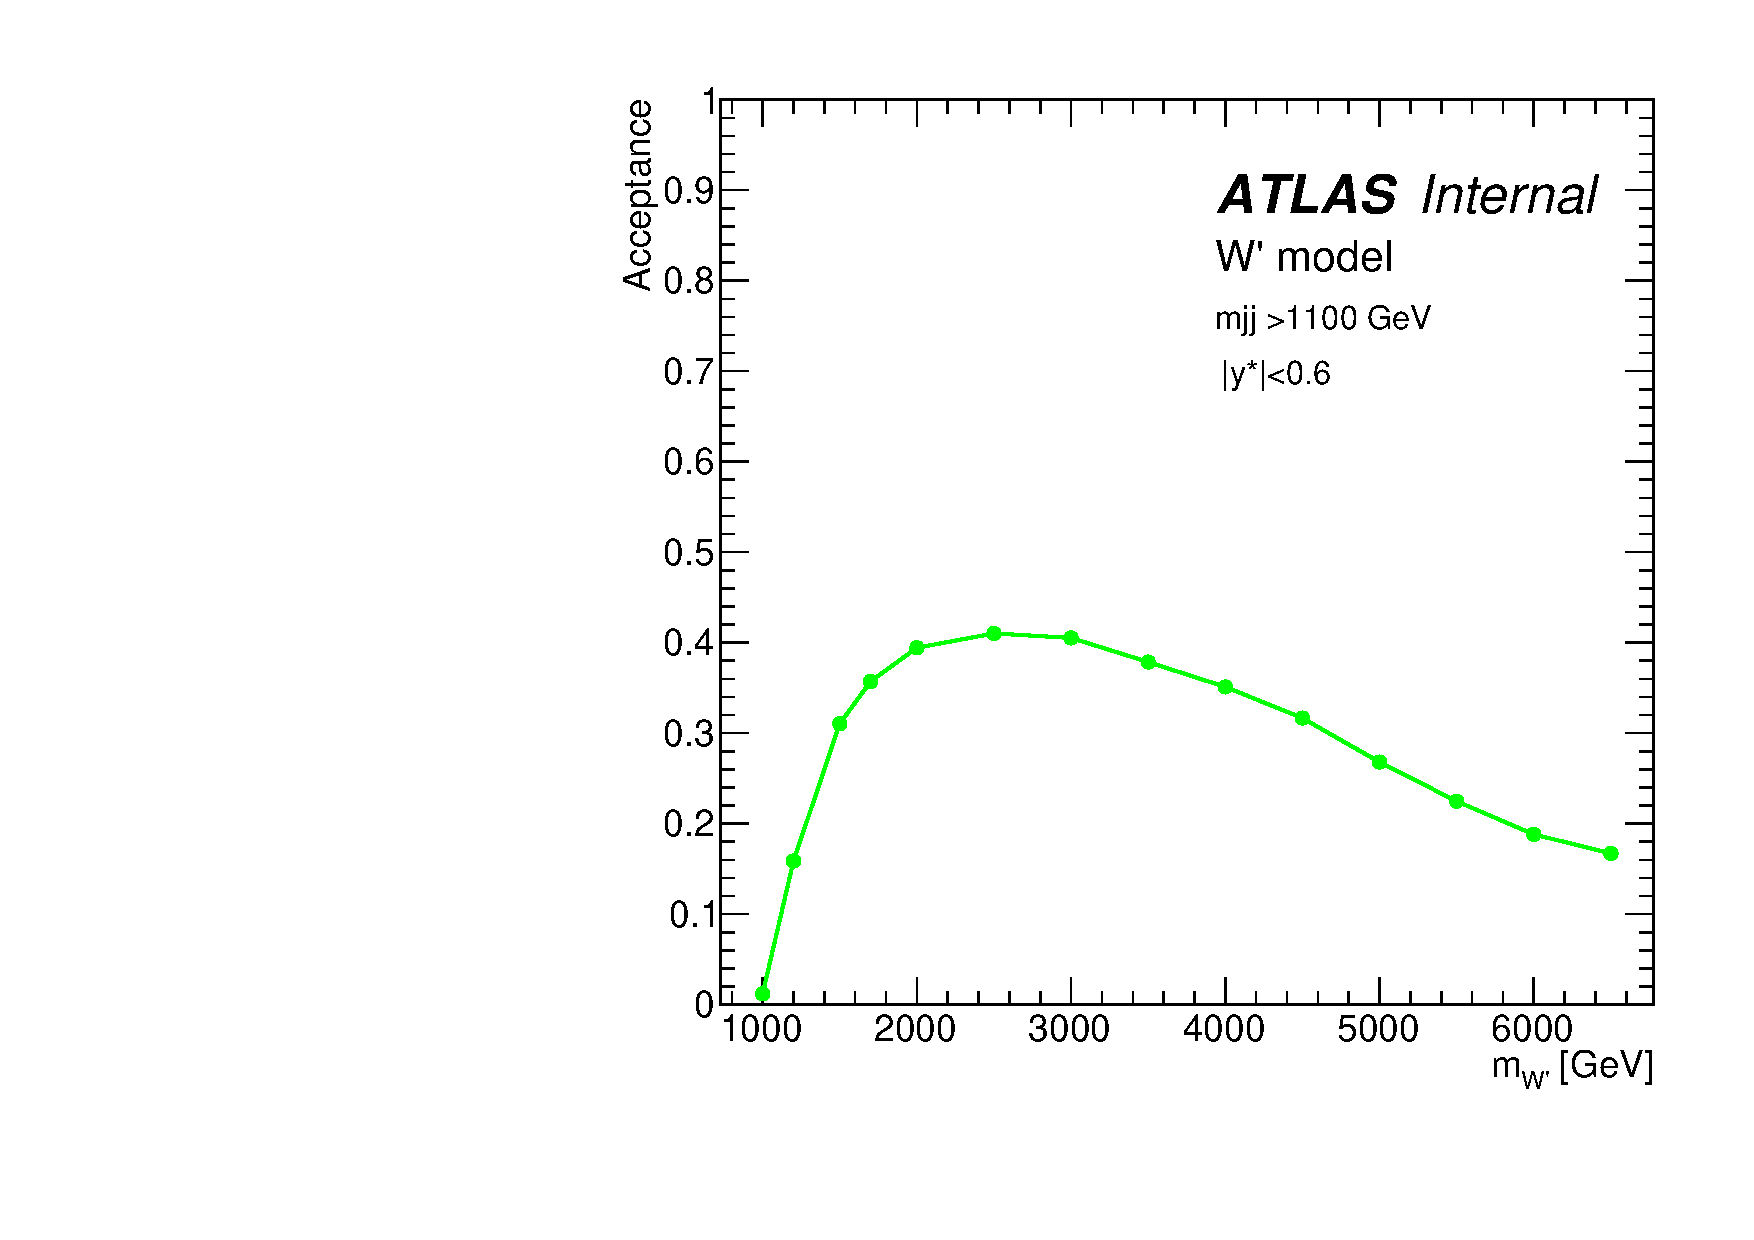
\includegraphics[width=0.9\textwidth]{figuresDijet/03-BenchmarkSignals/Acc_Wprime.pdf}
   \caption{}
   \label{fig:WPrime1}
  \end{subfigure}
  \begin{subfigure}{.5\textwidth}
  \centering
   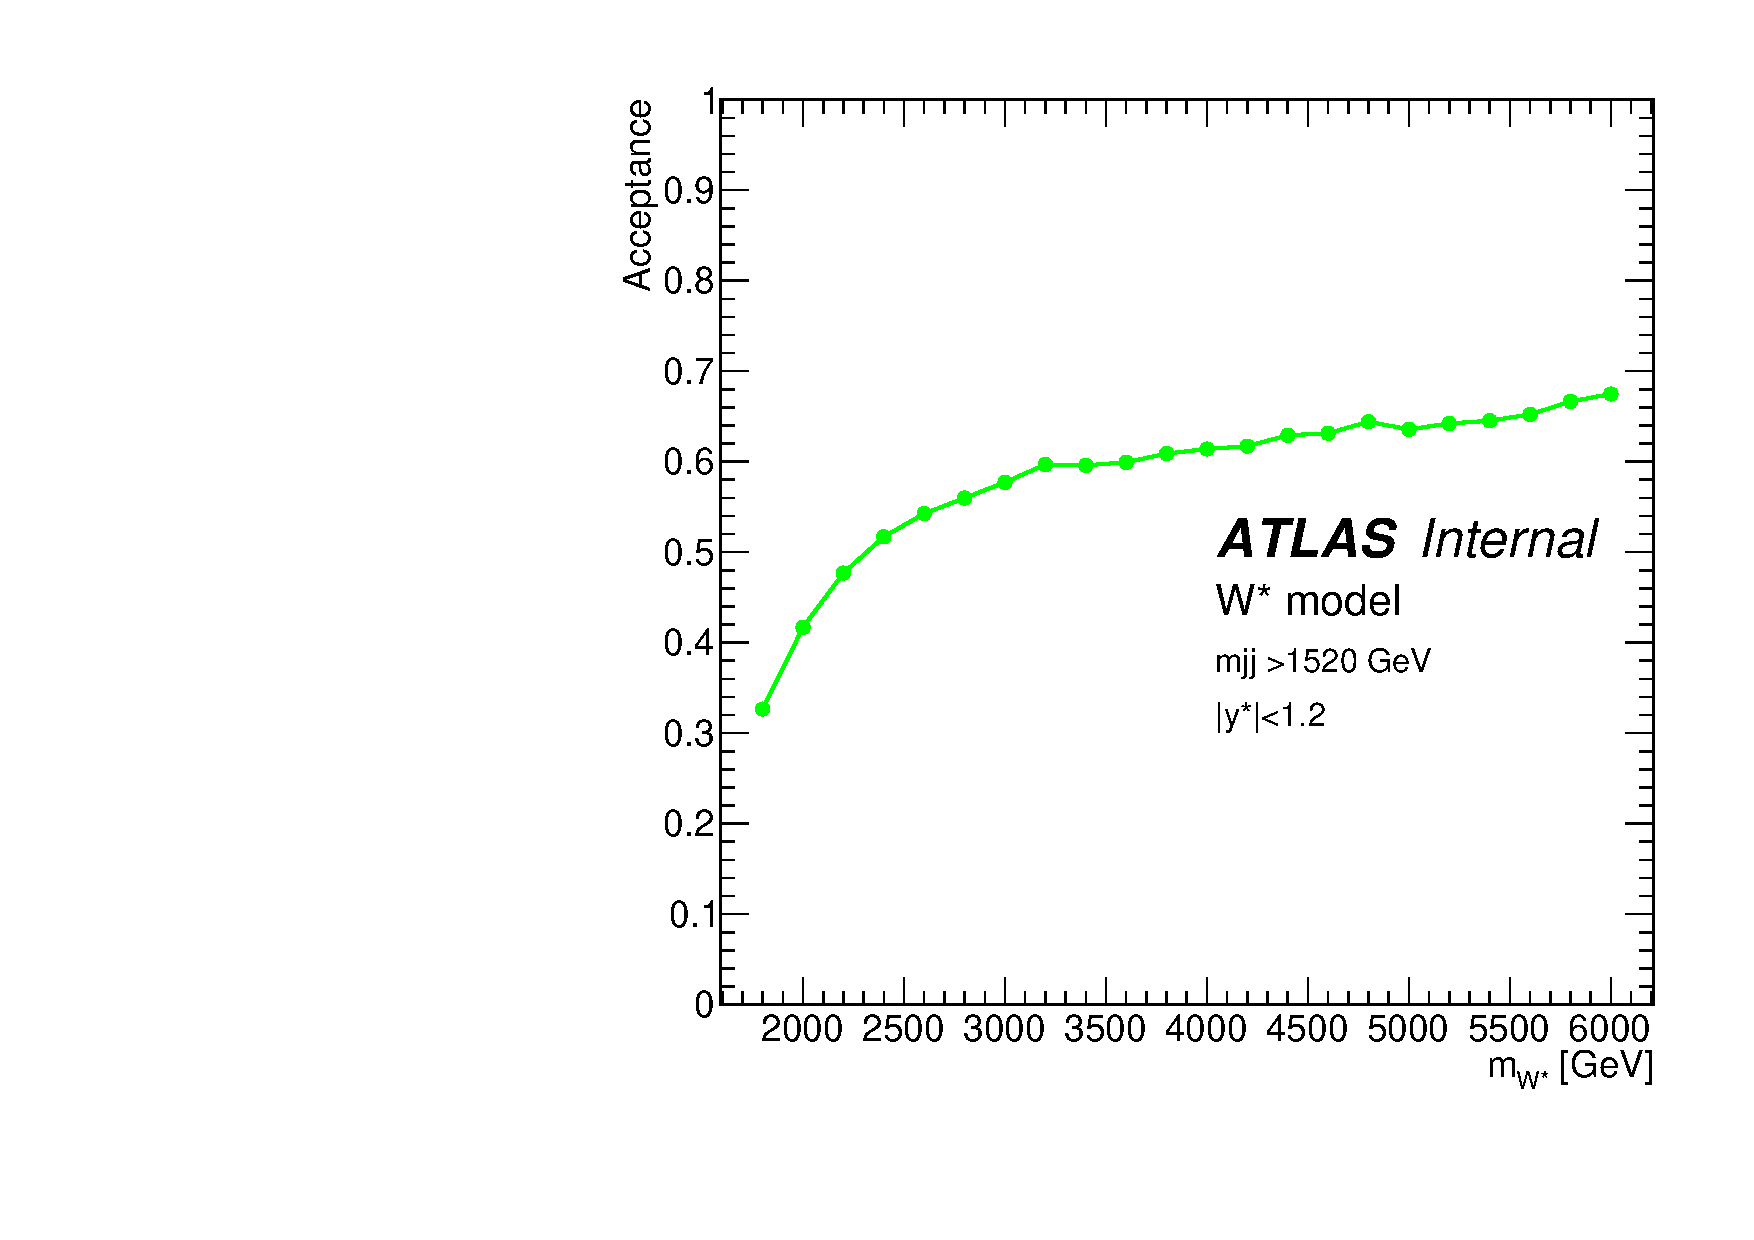
\includegraphics[width=0.9\textwidth]{figuresDijet/03-BenchmarkSignals/Acc_Wstar_yS1p2.pdf}
   \caption{}
   \label{fig:WStar1}
  \end{subfigure}
  \caption{
在全包含信号区,$q^*$、QBH、$W'$和$W^*$信号的接收度随着信号质量的变化.
(a) $q^*$;(b) QBH;(c) $W\prime$;(d) $W^*$。
  }
  \label{fig:ACCP}
\end{figure} 

\begin{figure}[thbp]
  \centering
  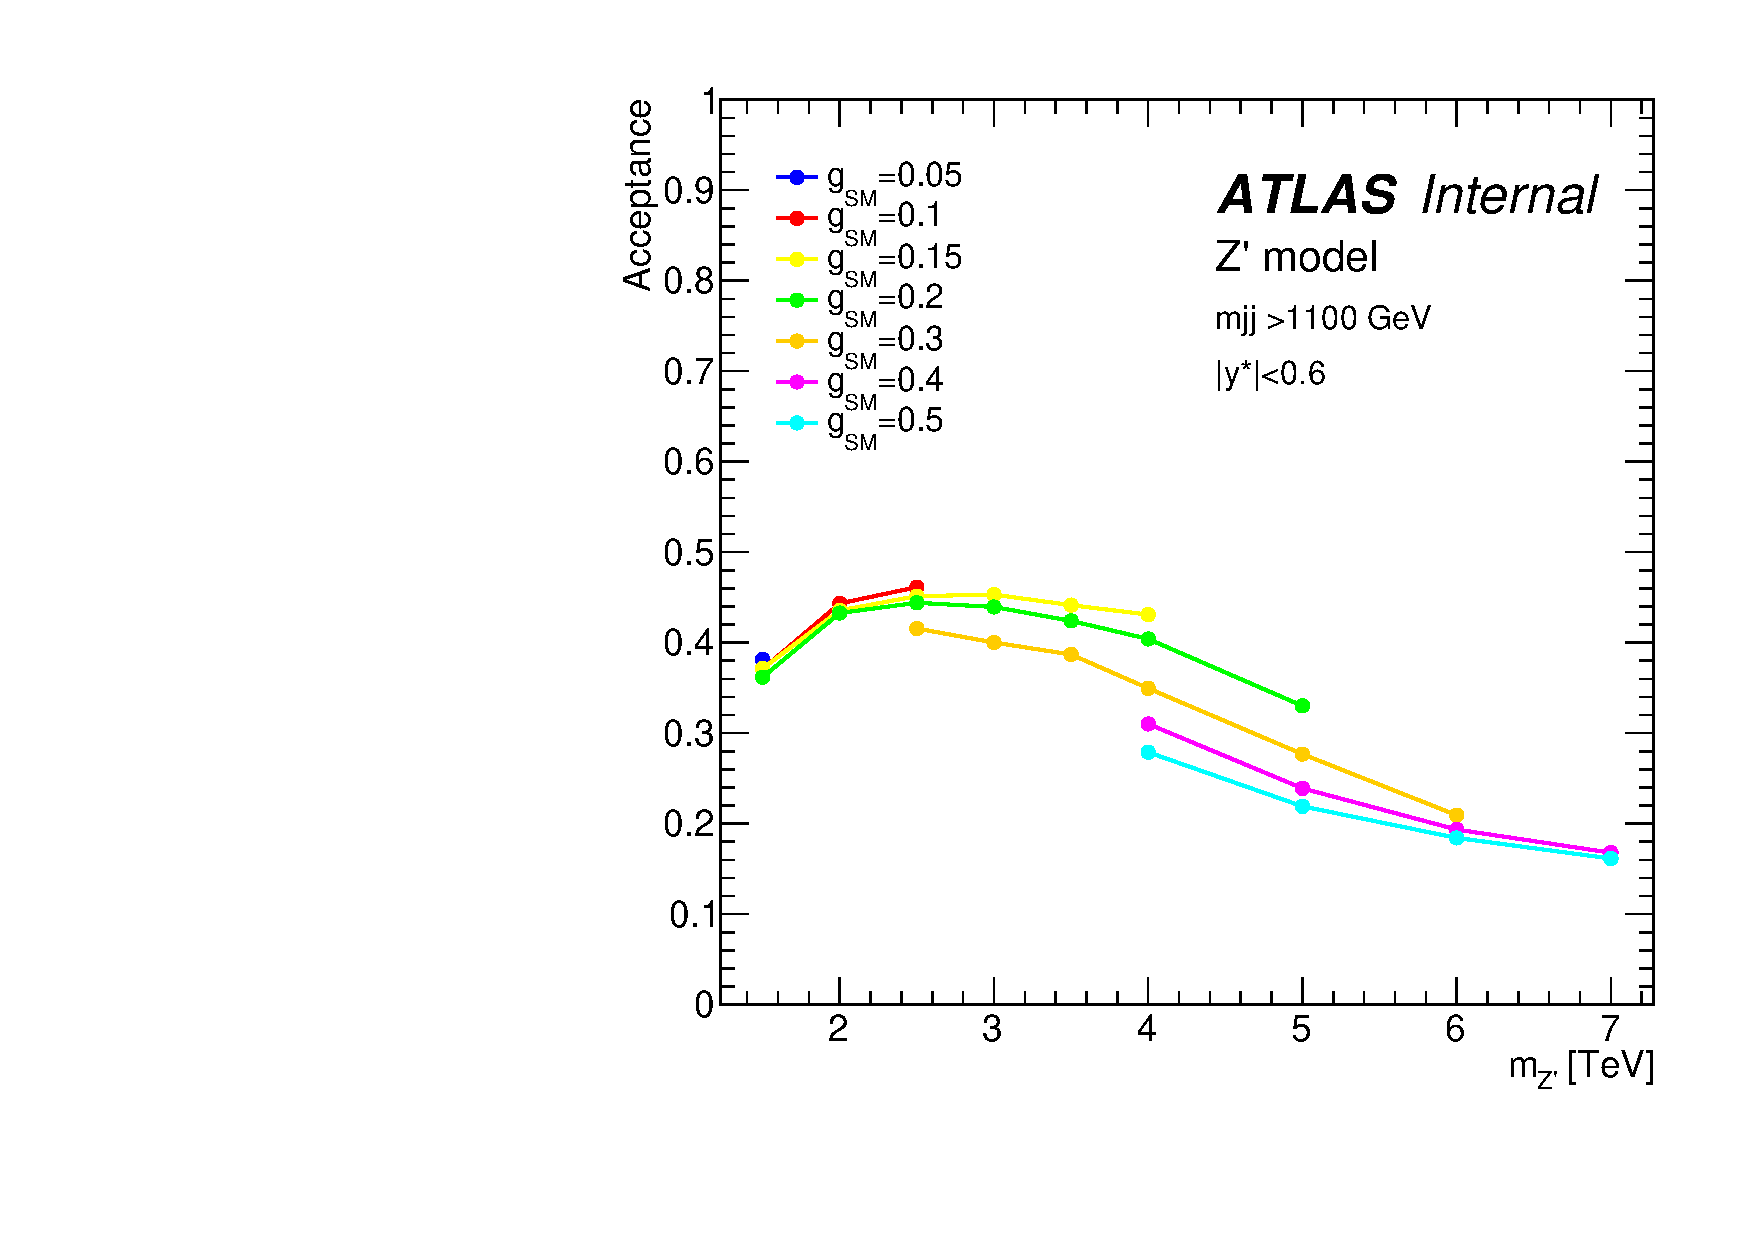
\includegraphics[width=0.75\textwidth]{figuresDijet/03-BenchmarkSignals/Acc_Zprime.pdf}
  \caption{ 在全包含信号区,$Z'$信号的接收度随着信号质量的变化。 }
  \label{fig:ACCPZ}
\end{figure}

图~\ref{fig:ACCPB}~展示的是1b和2b信号区的信号接收度乘以b-jet标定效率随着信号质量的变化,
这个分析所用的b-jet标定技术将在下一节~\ref{sec:DijetBtagging}~详细介绍。
其中圆点代表信号接收度随着信号质量的变化,正三角的点代表在1b信号区,
信号接收度乘以b-jet标定效率随着信号质量的变化,
倒三角的点代表在2b信号区,
信号接收度乘以b-jet标定效率随着信号质量的变化。
黑色代表$b^*$信号,红色代表DM $Z'(b\overline{b})$信号,
绿色代表SSM $Z'(b\overline{b})$信号,蓝色代表KK $G \rightarrow b\bar{b}$信号。
可以看出,在1b和2b信号区,
信号$b^*$、DM $Z'(b\overline{b})$和KK $G \rightarrow b\bar{b}$的接收度从$20\%$开始增加,
并在质量为2.5TeV时达到一个平稳值的$70\%$左右,
而SSM $Z'(b\overline{b})$信号在高质量区接收度较低,
是因为在高质量区时,
SSM $Z'$信号的不变质量的分布在低质量区的尾部拖的比较长。

 
 \begin{figure}[thbp]
  \centering
  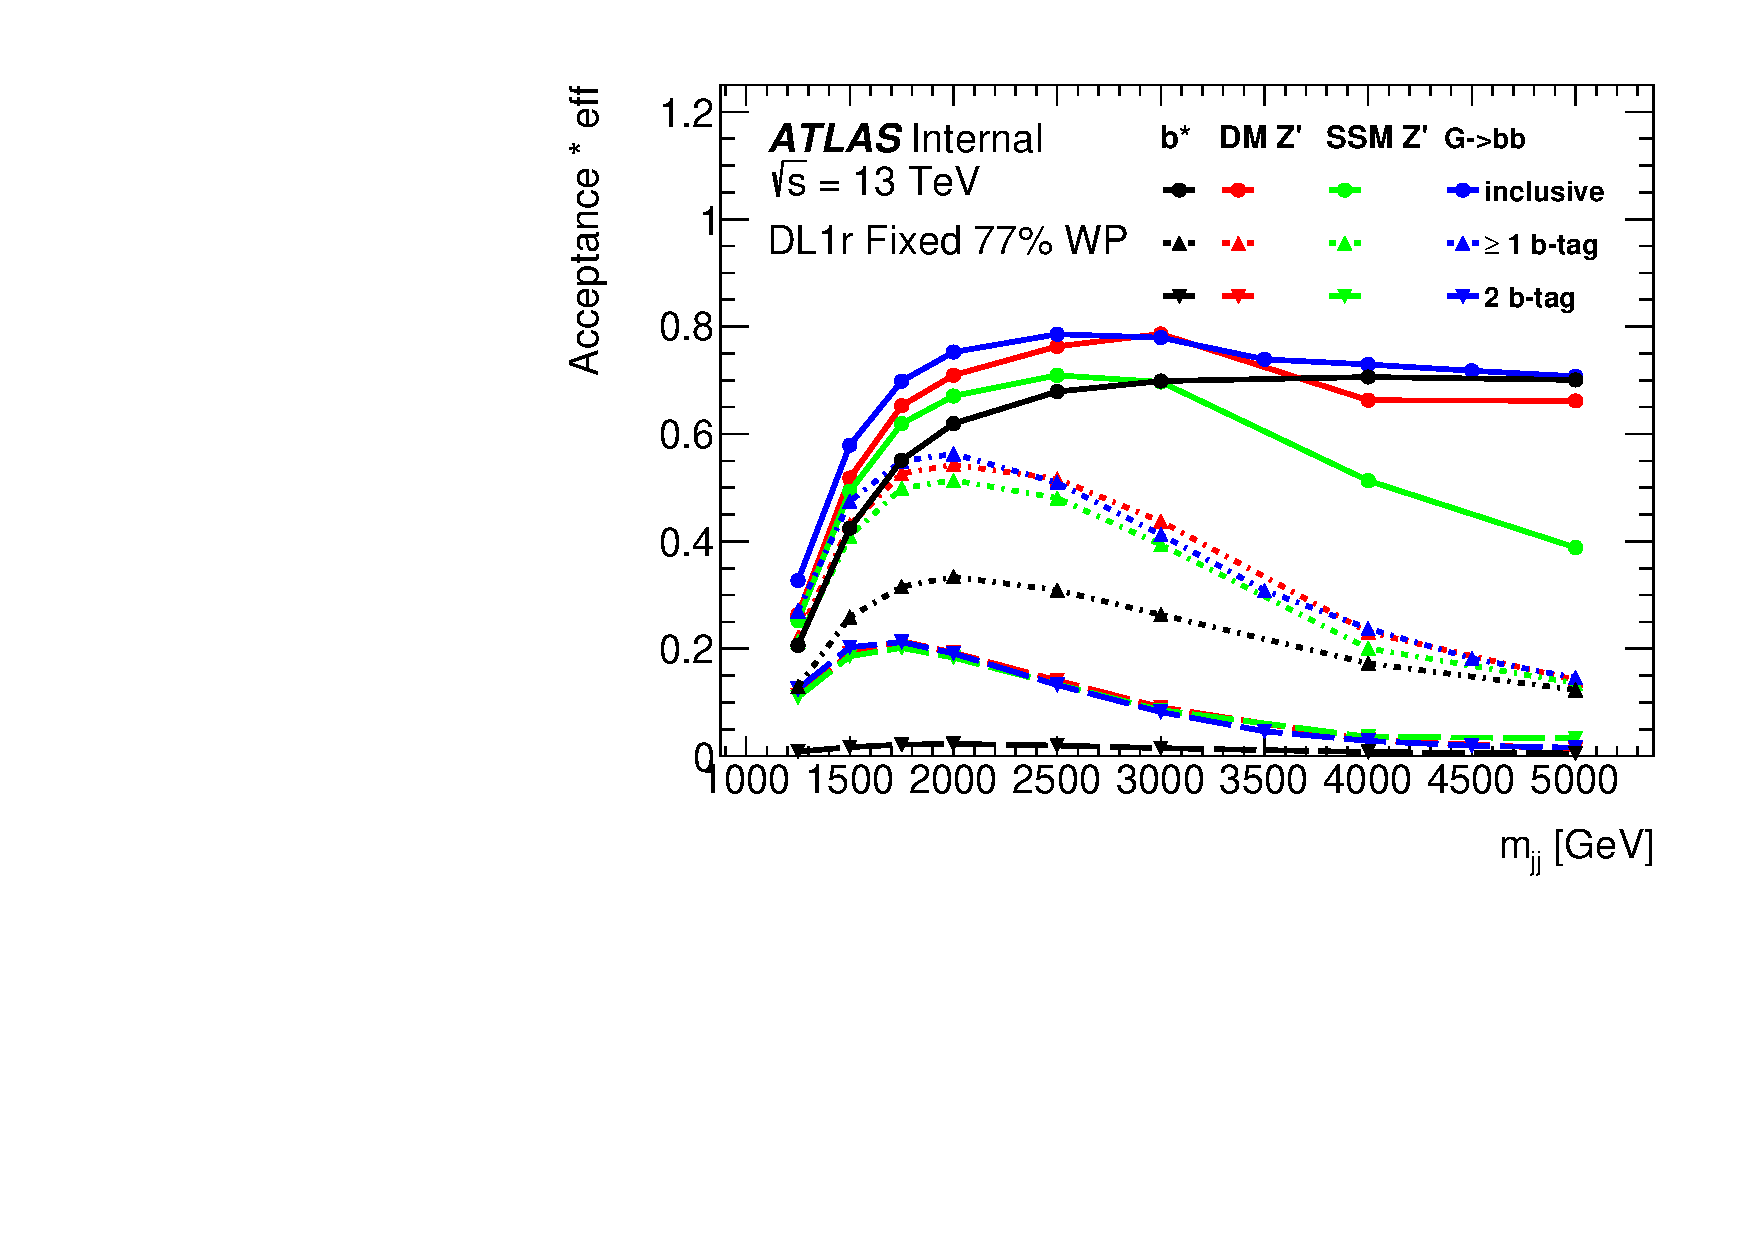
\includegraphics[width=0.75\textwidth]{figuresDijet/03-BenchmarkSignals/Acceff_DL1r_Fix77.pdf}
  \caption{ 在1b和2b信号区,信号接收度乘以b-jet标定效率随着信号质量的变化,
这个分析所用的b-jet标定技术将在下一节~\ref{sec:DijetBtagging}~详细介绍。
其中圆点代表信号接收度随着信号质量的变化,正三角的点代表在1b信号区,
信号接收度乘以b-jet标定效率随着信号质量的变化,
倒三角的点代表在2b信号区,
信号接收度乘以b-jet标定效率随着信号质量的变化。
黑色代表$b^*$信号,红色代表DM $Z'(b\overline{b})$信号,
绿色代表SSM $Z'(b\overline{b})$信号,蓝色代表KK $G \rightarrow b\bar{b}$信号。 }
  \label{fig:ACCPB}
\end{figure}
 
 
 
\subsection{$m_{jj}$分辨率}
\label{sec:DijetMjjBin}

对于$m_{jj}$的分bin,我们希望bin的总数量达到最大,从而能够探测到尽可能窄的新共振态,
但是,为了限制bin到bin之间事例的迁移带来的影响,bin宽需要大于探测器的分辨率。
因此首先我们需要找到探测器的分辨率,然后决定bin宽。

为了找到探测器的分辨率,
在多个$m_{jj}^{truth}$区间,对$m_{jj}^{reco}/m_{jj}^{truth}$比率的分布用一个高斯分布进行拟合,
然后,探测器的分辨率R可以由拟合出来的方法除以均值$R=\sigma/\mu$得到。
其中$m_{jj}^{reco}$是由MC模拟重建出来的事例中两个领头jet的不变质量,
利用与MC模拟重建出来的两个领头jet相关联的TH-jet,
可以计算相应的不变质量$m_{jj}^{truth}$,
其中TH-jet是通过产生子层面的真实粒子构建的,称为真实的jet,
为了与探测器响应相对应,要求这些真实粒子的寿命大于10ps,且不包含$\mu$和中微子,
随后以这些真实粒子为单元,用第~\ref{sec:JET}~小节与SR-jet重建相同的重建算法构建TH-jet,
随后通过第~\ref{sec:JET}~小节描述的“幻影”关联~\cite{Cacciari:2008gn}
的过程将MC模拟重建出来的jet与TH-jet的关联起来。

接下来,将探测器的分辨率R随着$m_{jj}^{truth}$变化的分布用函数:
\begin{equation} 
\label{eq:MJJR1}
R(m_{jj}^{truth})=\frac{a}{m_{jj}^{truth}}+\frac{b}{\sqrt{m_{jj}^{truth}}}+c
\end{equation}
进行拟合,用于对分辨率R的变化建模。
在领头jet横动量$p_T>150GeV$的初始筛选条件下,
边界946GeV略高于MC样本中$m_{jj}$分布的峰值,而且远低于用于分析的$m_{jj}$初始值。
于是,给定一个bin初始边界$m_{initial}=946GeV$之后,
用以下过程决定其他高质量区的bin边界:
\begin{enumerate}
  \item 对于给定的bin初始边界$m_{initial}$,计算相应的分辨率$R(m_{initial})$,
  然后推断该bin中心值为$m_{centre}=m_{initial}(1+\frac{1}{2}R(m_{initial}))$;
  \item 由推断的bin中心值$m_{center}$反过来计算bin左边的边界值
  $m_{lower}=m_{centre}(1-\frac{1}{2}R(m_{centre}))$;
  \item 检查$m_{initial}$和$m_{lower}$之间的相对差异是否小于0.1\%,
  如果差异大于0.1\%且$m_{lower}>m_{initial}$,则使$m_{centre}=m_{centre}-0.01GeV$,然后重复步骤2中的过程;
 如果差异大于0.1\%且$m_{lower}<m_{initial}$,则使$m_{centre}=m_{centre}+0.01GeV$,然后重复步骤2中过程;
  \item 一旦$m_{initial}$和$m_{lower}$之间的相对差异小于0.1,固定$m_{centre}$,并计算该bin右边的边界值
  $m_{upper}=m_{centre}(1+\frac{1}{2}R(m_{centre}))$,并四舍五入到最接近的整数GeV;
  \item 然后使$m_{initial}=m_{upper}$,并重复以上过程。
\end{enumerate}















\section{b-jet标定算法}
\label{sec:DijetBtagging}

关于这个分析所用到的b-jet标定技术,这是在ATLAS合作组内部分析中第一次使用基于深度学习神经网络(deep-learning neural network)的DL1r算法来~\cite{DLOR1,DLOR2}标定b-jet,
DL1r算法是基于b-jet在内部探测器中重建时一些独特的性质而构建的高级算法,在第~\ref{sec:BJET}~小节有详细介绍,
而且用于训练DL1r的参数集中还包括由递归神经网络(recurrent neural network)构造的区分变量(RNNIP)~\cite{ATL-PHYS-PUB-2017-003},
这些区分变量是用来表征源自同一个$b$强子的那些径迹之间的空间和运动学关联性,这种方法主要能提升高横动量jet的标定性能。
通过对1b和2b信号区中不同的信号模型和相应质量点的信号灵敏度进行研究,我们采用了DL1r算法的b-jet标定效率为$77\%$的工作点,
其中工作点是通过在区分因子分布上的一个截断值来定义的,所选择的截断值对应于MC样本$t\bar{t}$中的一个特定的b-jet标定效率~\cite{ATL-PHYS-PUB-2017-013}。

\subsection{算法灵敏度}
\label{sec:DijetBtagging1}

在确定b-jet标定算法和工作点的时候,我们选择了三个高级标定算法DL1、DL1r和DL1rmu
在四个不同的工作点60\%、70\%、77\%和85\%下进行信号灵敏度
\footnote{信号灵敏度定义为$S/\sqrt{B}$,其中S和B分别是区间中信号和本底的事例数。}的对比研究。
这三种算法在第~\ref{sec:JET}~小节有简要介绍。
表~\ref{tab:SenZ1p5TeV}-\ref{tab:SenZ5TeV}~是使用2b信号区的DM $Z\prime$信号在不同信号质量下所做灵敏度研究的一系列结果:
\begin{itemize}
	\item 表~\ref{tab:SenZ1p5TeV}~是使用质量为1.5TeV的DM $Z\prime$信号测试各个b-jet标定算法的灵敏度得到的结果,考虑的质量区间为1.378-1.573TeV;
	\item 表~\ref{tab:SenZ2TeV}~是使用质量为2TeV的DM $Z\prime$信号测试各个b-jet标定算法的灵敏度得到的结果,考虑的质量区间为1.785 - 2.114TeV;
	\item 表~\ref{tab:SenZ2p5TeV}~是使用质量为2.5TeV的DM $Z\prime$信号测试各个b-jet标定算法的灵敏度得到的结果,考虑的质量区间为2.267 - 2.659TeV;
	\item 表~\ref{tab:SenZ3TeV}~是使用质量为3TeV的DM $Z\prime$信号测试各个b-jet标定算法的灵敏度得到的结果,考虑的质量区间为2.719 - 3.1TeV;
	\item 表~\ref{tab:SenZ4TeV}~是使用质量为4TeV的DM $Z\prime$信号测试各个b-jet标定算法的灵敏度得到的结果,考虑的质量区间为3.672 - 4.07TeV;
	\item 表~\ref{tab:SenZ5TeV}~是使用质量为5TeV的DM $Z\prime$信号测试各个b-jet标定算法的灵敏度得到的结果,考虑的质量区间为4.595 - 5.074TeV。
\end{itemize}
从表中可以看到可以看到性能最好的标定算法是DL1r,而且大部分情况中在b-jet标定效率为$77\%$的工作点下灵敏度最高。

%ZPrime

\begin{table}[ht]
	\begin{center}
		\begin{tabular}{|c|c|c|c|c|}\hline
			Tagger       & WP          & Signal(S)    & $\sqrt{Background(B)}$    & S/$\sqrt{B}$ \\\hline
			DL1          & Fix 85      & 7239.83      & 352.07        & 20.56        \\
			DL1          & Fix 77      & 4151.16      & 148.90        & 27.88        \\
			DL1          & Fix 70      & 2655.21      & 98.01         & 27.09        \\
			DL1          & Fix 60      & 1445.55      & 65.57         & 22.04        \\
			\hline
			DL1r          & Fix 85      & 8477.72      & 390.54        & 21.71        \\
			DL1r          & Fix 77      & 5159.21      & 166.65        & 30.96        \\
			DL1r          & Fix 70      & 3399.15      & 112.75        & 30.15        \\
			DL1r          & Fix 60      & 1556.43      & 68.59         & 22.69        \\
			\hline
			DL1rmu          & Fix 85      & 6945.48      & 281.68        & 24.66        \\
			DL1rmu          & Fix 77      & 4302.37      & 143.26        & 30.03        \\
			DL1rmu          & Fix 70      & 2796.34      & 101.68        & 27.50        \\
			DL1rmu          & Fix 60      & 1330.63      & 60.88         & 21.86        \\
			\hline
		\end{tabular}
	\end{center}
	\caption{使用2b信号区的质量为1.5TeV的DM $Z\prime$信号测试各个b-jet标定算法的灵敏度,所选质量区间为1.378 - 1.573TeV。}
	\label{tab:SenZ1p5TeV}
\end{table}%

\begin{table}[ht]
	\begin{center}
		\begin{tabular}{|c|c|c|c|c|}\hline
			Tagger       & WP          & Signal(S)    & $\sqrt{Background(B)}$    & S/$\sqrt{B}$ \\
			\hline
			DL1          & Fix 85      & 1775.24     & 205.23        & 8.65        \\
			DL1          & Fix 77      & 686.94      & 65.90         & 10.42        \\
			DL1          & Fix 70      & 362.93      & 38.38         & 9.46        \\
			DL1          & Fix 60      & 152.28      & 21.58         & 7.06        \\
			\hline
			DL1r          & Fix 85      & 2364.88      & 233.62       & 10.12        \\
			DL1r          & Fix 77      & 1074.68      & 80.53        & 13.34        \\
			DL1r          & Fix 70      & 583.31       & 47.80        & 12.20        \\
			DL1r          & Fix 60      & 218.93       & 24.55        & 8.92        \\
			\hline
			DL1rmu          & Fix 85      & 1726.10     & 160.96       & 10.72        \\
			DL1rmu          & Fix 77      & 805.64      & 65.94        & 12.22        \\
			DL1rmu          & Fix 70      & 468.50      & 41.88        & 11.19        \\
			DL1rmu          & Fix 60      & 161.03      & 20.07        & 8.02        \\
			\hline
		\end{tabular}
	\end{center}
	\caption{使用2b信号区的质量为2TeV的DM $Z\prime$信号测试各个b-jet标定算法的灵敏度,所选质量区间为1.785 - 2.114TeV;	}
	\label{tab:SenZ2TeV}
\end{table}

\begin{table}[ht]
	\begin{center}
		\begin{tabular}{|c|c|c|c|c|}\hline
			Tagger       & WP          & Signal(S)    & $\sqrt{Background(B)}$    & S/$\sqrt{B}$ \\
			\hline
			DL1          & Fix 85      & 333.68     & 100.46        & 3.32        \\
			DL1          & Fix 77      & 78.90      & 23.40         & 3.37        \\
			DL1          & Fix 70      & 35.46      & 12.02         & 2.95        \\
			DL1          & Fix 60      & 11.07      & 6.21          & 1.78        \\
			\hline
			DL1r          & Fix 85      & 527.50      & 115.69       & 4.56        \\
			DL1r          & Fix 77      & 170.98      & 31.73        & 5.39        \\
			DL1r          & Fix 70      & 74.14       & 16.60        & 4.47        \\
			DL1r          & Fix 60      & 20.46       & 7.33         & 2.79        \\
			\hline
			DL1rmu          & Fix 85      & 346.72     & 78.48       & 4.42        \\
			DL1rmu          & Fix 77      & 116.18     & 26.19       & 4.44        \\
			DL1rmu          & Fix 70      & 55.77      & 14.72       & 3.79        \\
			DL1rmu          & Fix 60      & 14.29      & 6.24        & 2.29        \\
			\hline
		\end{tabular}
	\end{center}
	\caption{使用2b信号区的质量为2.5TeV的DM $Z\prime$信号测试各个b-jet标定算法的灵敏度,所选质量区间为2.267 - 2.659TeV。}
	\label{tab:SenZ2p5TeV}
\end{table}

\begin{table}[ht]
	\begin{center}
		\begin{tabular}{|c|c|c|c|c|}\hline
			Tagger       & WP          & Signal(S)    & $\sqrt{Background(B)}$    & S/$\sqrt{B}$ \\
			\hline
			DL1          & Fix 85      & 69.86     & 49.39        & 1.41        \\
			DL1          & Fix 77      & 9.09      & 8.98         & 1.01        \\
			DL1          & Fix 70      & 3.49      & 4.17         & 0.84        \\
			DL1          & Fix 60      & 0.90      & 1.98         & 0.45        \\
			\hline
			DL1r          & Fix 85      & 129.02     & 58.66       & 2.20        \\
			DL1r          & Fix 77      & 26.42      & 13.70       & 1.93        \\
			DL1r          & Fix 70      & 8.82       & 6.29        & 1.40        \\
			DL1r          & Fix 60      & 2.06       & 2.84        & 0.73        \\
			\hline
			DL1rmu          & Fix 85      & 78.06     & 39.00       & 2.00        \\
			DL1rmu          & Fix 77      & 18.45     & 11.33       & 1.63        \\
			DL1rmu          & Fix 70      & 7.12      & 5.94        & 1.20        \\
			DL1rmu          & Fix 60      & 1.43      & 2.38        & 0.60        \\
			\hline
		\end{tabular}
	\end{center}
	\caption{使用2b信号区的质量为3TeV的DM $Z\prime$信号测试各个b-jet标定算法的灵敏度,所选质量区间为2.719 - 3.1TeV。}
	\label{tab:SenZ3TeV}
\end{table}

\begin{table}[ht]
	\begin{center}
		\begin{tabular}{|c|c|c|c|c|}\hline
			Tagger       & WP          & Signal(S)    & $\sqrt{Background(B)}$    & S/$\sqrt{B}$ \\
			\hline
			DL1          & Fix 85      & 2.434      & 10.898        & 0.22        \\
			DL1          & Fix 77      & 0.148      & 1.144         & 0.13        \\
			DL1          & Fix 70      & 0.045      & 0.350         & 0.13        \\
			DL1          & Fix 60      & 0.0065     & 0.133         & 0.05        \\
			\hline
			DL1r          & Fix 85      & 6.389       & 14.145       & 0.45        \\
			DL1r          & Fix 77      & 0.561       & 2.341        & 0.24        \\
			DL1r          & Fix 70      & 0.116       & 0.876        & 0.13        \\
			DL1r          & Fix 60      & 0.0153      & 0.308        & 0.05        \\
			\hline
			DL1rmu          & Fix 85      & 3.583     & 8.894       & 0.40        \\
			DL1rmu          & Fix 77      & 0.480     & 2.094       & 0.23        \\
			DL1rmu          & Fix 70      & 0.107     & 1.027       & 0.10        \\
			DL1rmu          & Fix 60      & 0.0153    & 0.346       & 0.04        \\
			\hline
		\end{tabular}
	\end{center}
	\caption{使用2b信号区的质量为4TeV的DM $Z\prime$信号测试各个b-jet标定算法的灵敏度,所选质量区间为3.672 - 4.07TeV;}
	\label{tab:SenZ4TeV}
\end{table}

\begin{table}[ht]
	\begin{center}
		\begin{tabular}{|c|c|c|c|c|}\hline
			Tagger       & WP          & Signal(S)    & $\sqrt{Background(B)}$    & S/$\sqrt{B}$ \\
			\hline
			DL1          & Fix 85      & 0.0698      & 2.2834         & 0.03        \\
			DL1          & Fix 77      & 0.0022      & 0.1990         & 0.01        \\
			DL1          & Fix 70      & 0.0003      & 0.0643         & 0.005        \\
			DL1          & Fix 60      & 0.0003      & 0              & --           \\
			\hline
			DL1r          & Fix 85      & 0.2751       & 3.4954        & 0.08        \\
			DL1r          & Fix 77      & 0.0097       & 0.4109        & 0.02        \\
			DL1r          & Fix 70      & 0.0028       & 0.1440        & 0.02        \\
			DL1r          & Fix 60      & 0.0003       & 0.0483        & 0.006        \\
			\hline
			DL1rmu          & Fix 85      & 0.1580     & 2.1432       & 0.073        \\
			DL1rmu          & Fix 77      & 0.0097     & 0.4667       & 0.02        \\
			DL1rmu          & Fix 70      & 0.0025     & 0.2434       & 0.01        \\
			DL1rmu          & Fix 60      & 0.0013     & 0.1386       & 0.01        \\
			\hline
		\end{tabular}
	\end{center}
	\caption{使用2b信号区的质量为5TeV的DM $Z\prime$信号测试各个b-jet标定算法的灵敏度,所选质量区间为4.595 - 5.074TeV。}
	\label{tab:SenZ5TeV}
\end{table}

%BStar

我们还研究了不同工作点下的DL1r算法在1b信号区的灵敏度,
表~\ref{tab:Sensbstar1p5TeV}-~\ref{tab:Sensbstar5TeV}~是使用1b信号区的$b^*$信号在不同信号质量下所做灵敏度研究的一系列结果:
\begin{itemize}
	 \item 表~\ref{tab:Sensbstar1p5TeV}~是使用质量为1.5TeV的$b^*$信号测试各个b-jet标定算法的灵敏度得到的结果,考虑的质量区间为1.378 - 1.573TeV;
	\item 表~\ref{tab:Sensbstar2TeV}~是使用质量为2TeV的$b^*$信号测试各个b-jet标定算法的灵敏度得到的结果,考虑的质量区间为1.785 - 2.114TeV;
	\item 表~\ref{tab:Sensbstar2p5TeV}~是使用质量为2.5TeV的$b^*$信号测试各个b-jet标定算法的灵敏度得到的结果,考虑的质量区间为2.267 - 2.659TeV;
	\item 表~\ref{tab:Sensbstar5TeV}~是使用质量为5TeV的$b^*$信号测试各个b-jet标定算法的灵敏度得到的结果,考虑的质量区间为4.595 - 5.074TeV;
\end{itemize}
可以看到在77\%的工作点下仍具有很高的灵明度,因此最终选择了77\%同时作为1b和2b信号区的工作点。

\begin{table}[ht]
        \begin{center}
                \begin{tabular}{|c|c|c|c|c|}\hline
                        Tagger       & WP          & Signal(S)    & $\sqrt{Background(B)}$    & S/$\sqrt{B}$ \\\hline
                        DL1r          & Fix 85      & 62822.3       &   1427.81      & 44.0     \\
                        DL1r          & Fix 77      & 48707.9      &  897.43       &   54.28    \\
                        DL1r          & Fix 70      & 9488.9     &  697.08      &  56.65      \\
                        DL1r          & Fix 60      & 27044.6       &  513.68        & 52.65        \\
                        \hline
                \end{tabular}
        \end{center}
        \caption{使用1b信号区的质量为1.5TeV的$b^*$信号测试各个b-jet标定算法的灵敏度,所选质量区间为1.378 - 1.573TeV。}
        \label{tab:Sensbstar1p5TeV}
\end{table}%


\begin{table}[ht]
        \begin{center}
                \begin{tabular}{|c|c|c|c|c|}\hline
                        Tagger       & WP          & Signal(S)    & $\sqrt{Background(B)}$    & S/$\sqrt{B}$ \\\hline
                        DL1r          & Fix 85      & 13414.8      & 814.838        & 16.46       \\
                        DL1r          & Fix 77      & 9123.77      & 469.647       & 19.43    \\
                        DL1r          & Fix 70      & 6751.46      &  346.79       & 19.41       \\
                        DL1r          & Fix 60      & 4163.57     & 239.386         & 17.39    \\
                        \hline
                \end{tabular}
        \end{center}
        \caption{使用1b信号区的质量为2TeV的$b^*$信号测试各个b-jet标定算法的灵敏度,所选质量区间为1.785 - 2.114TeV;}
        \label{tab:Sensbstar2TeV}
\end{table}%

\begin{table}[ht]
        \begin{center}
                \begin{tabular}{|c|c|c|c|c|}\hline
                        Tagger       & WP          & Signal(S)    & $\sqrt{Background(B)}$    & S/$\sqrt{B}$ \\\hline
                        DL1r          & Fix 85      & 2380.96      &  403.956        & 5.89         \\
                        DL1r          & Fix 77      & 1350.94       & 212.474          & 6.36         \\
                        DL1r          & Fix 70      & 891.97     & 149.332      & 5.97       \\
                        DL1r          & Fix 60      & 488.16     &  97.5462       & 5.0     \\
                        \hline
                \end{tabular}
        \end{center}
        \caption{使用1b信号区的质量为2.5TeV的$b^*$信号测试各个b-jet标定算法的灵敏度,所选质量区间为2.267 - 2.659TeV; }
        \label{tab:Sensbstar2p5TeV}
\end{table}%


\begin{table}[ht]
        \begin{center}
                \begin{tabular}{|c|c|c|c|c|}\hline
                        Tagger       & WP          & Signal(S)    & $\sqrt{Background(B)}$    & S/$\sqrt{B}$ \\\hline
                        DL1r          & Fix 85      & 0.8067    &   18.0767       & 0.045        \\
                        DL1r          & Fix 77      & 0.1602      &  6.360         & 0.025       \\
                        DL1r          & Fix 70      & 0.0694     & 3.774       & 0.018       \\
                        DL1r          & Fix 60      & 0.0218      & 1.980         & 0.011       \\
                        \hline
                \end{tabular}
        \end{center}
        \caption{使用1b信号区的质量为5TeV的$b^*$信号测试各个b-jet标定算法的灵敏度,所选质量区间为4.595 - 5.074TeV;}
        \label{tab:Sensbstar5TeV}
\end{table}%


\subsection{$|y^*|$优化}
\label{sec:DijetBtagging3}

上一节所展示的1b和2b信号区中的$|y^*|$筛选条件是
基于选中的DL1r算法对其中DM $Z\prime\rightarrow b\bar{b}$信号和KK $G \rightarrow b\bar{b}$信号的灵敏度进行优化得到的结果,
如图~\ref{fig:Btag_ystar}~所示,分别是DM $Z\prime\rightarrow b\bar{b}$信号和KK $G \rightarrow b\bar{b}$信号的灵敏度随着$|y^*|$的变化关系,
优化后的筛选条件是$|y^*|<0.8$。

\begin{figure}[!thbp]
  \begin{subfigure}{.5\textwidth}
  \centering
  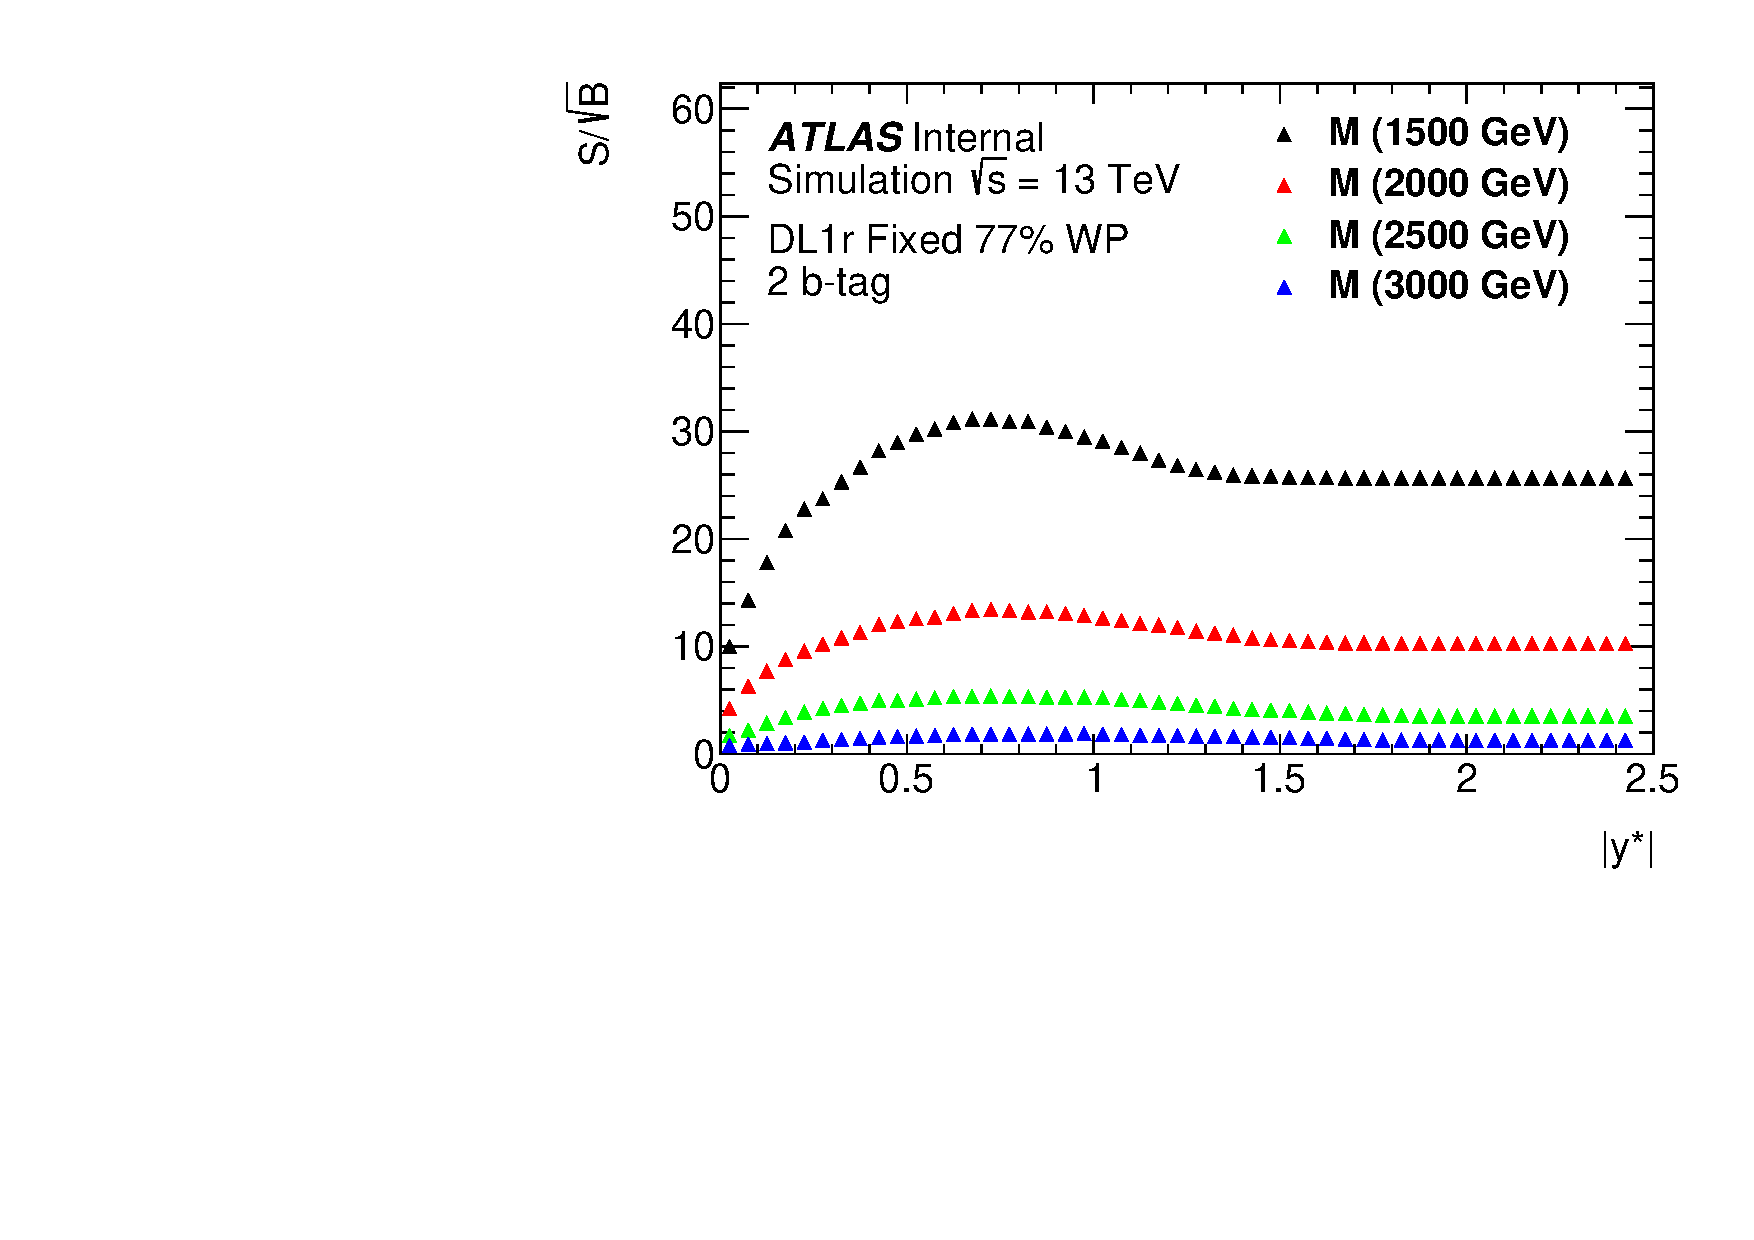
\includegraphics[width=0.9\textwidth]{figuresDijet/03-BenchmarkSignals/Ystar_DMZ_DL1r_Fixed77.pdf}
  \caption{DM $Z\prime \rightarrow  b\bar{b}$ 信号}
  \end{subfigure}
  \begin{subfigure}{.5\textwidth}
  \centering
  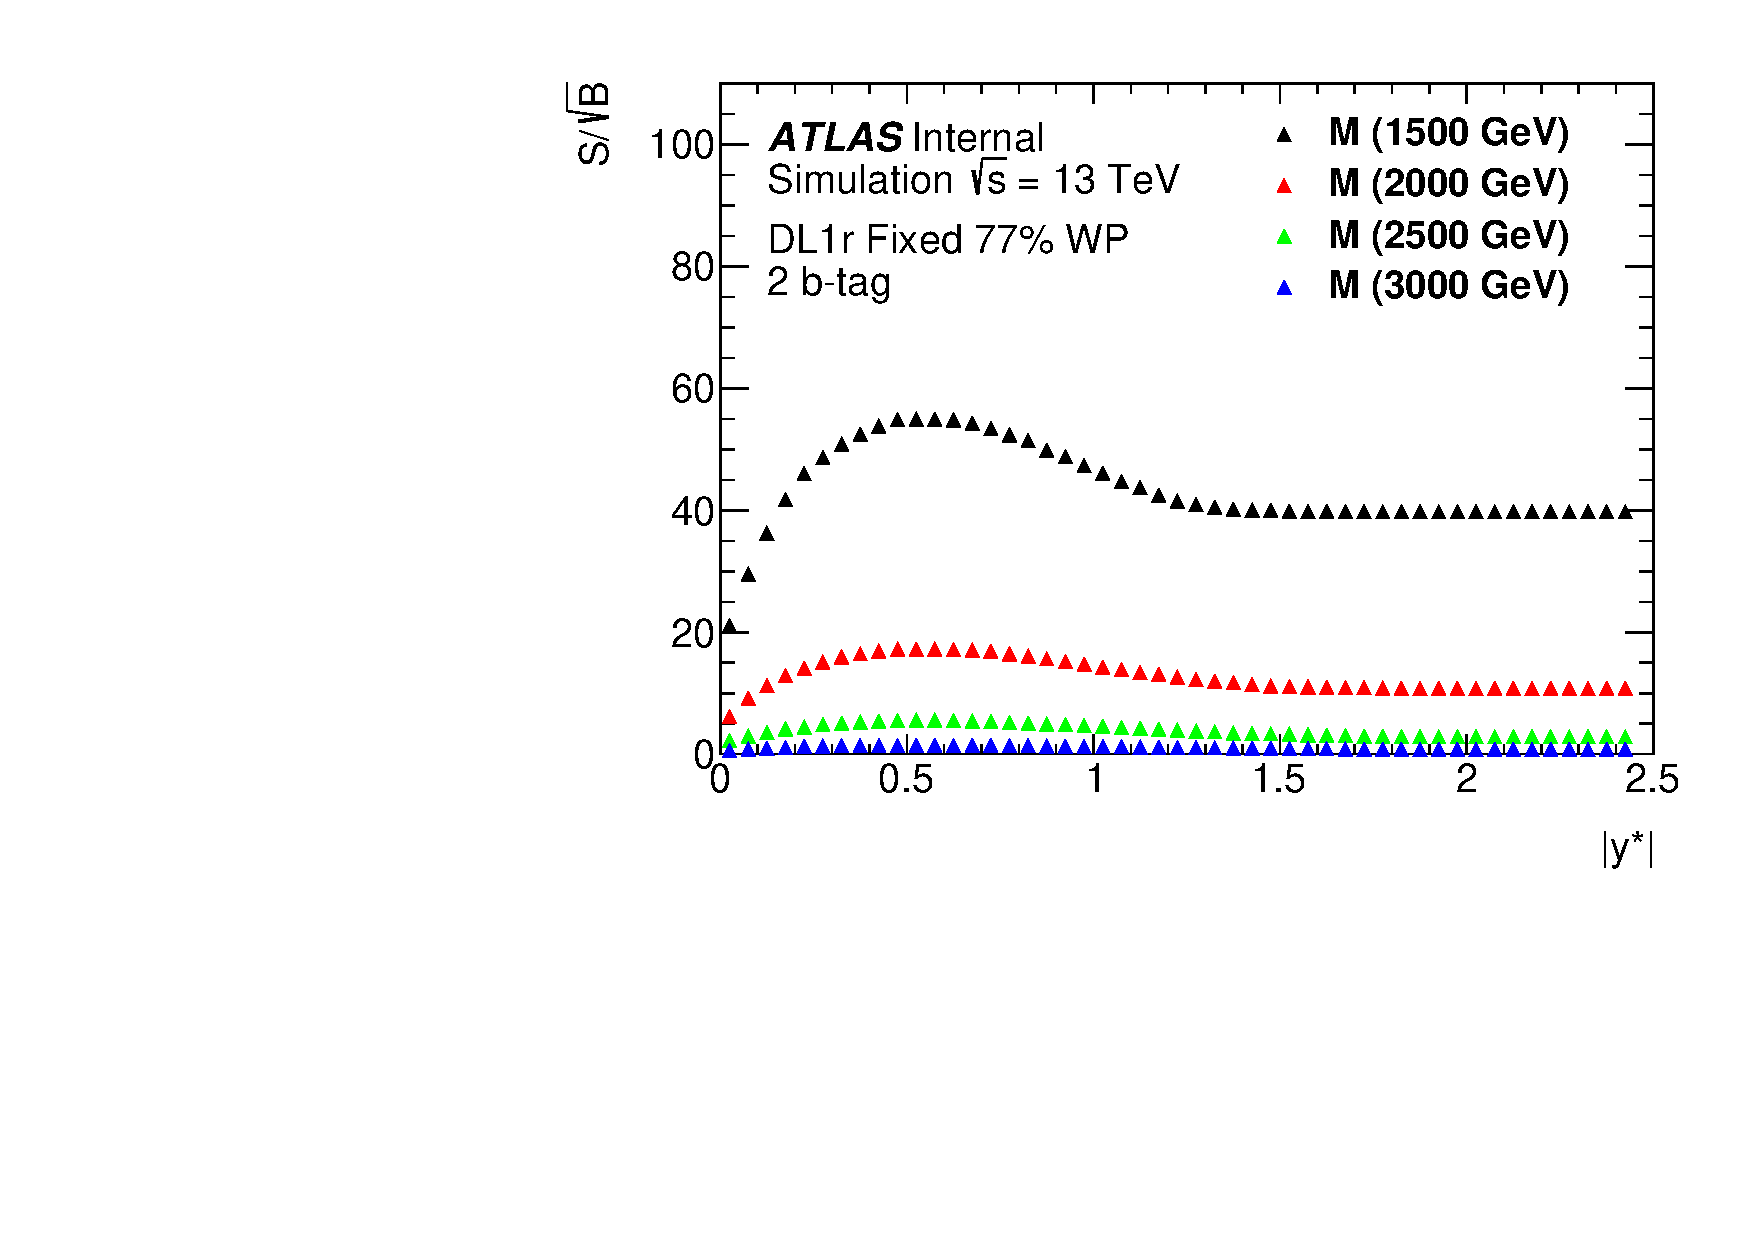
\includegraphics[width=0.9\textwidth]{figuresDijet/03-BenchmarkSignals/Ystar_Gbb_DL1r_Fixed77.pdf}
  \caption{KK G $\rightarrow b\bar{b}$ 信号}
  \end{subfigure}
\caption{
DM $Z\prime\rightarrow b\bar{b}$信号和KK G $\rightarrow b\bar{b}$信号的灵敏度随着$|y^*|$的变化关系。
}
\label{fig:Btag_ystar}
\end{figure}


\subsection{算法性能}
\label{sec:DijetBtagging2}

另外,我们还对三个高级标定算法DL1、DL1r和DL1rmu在b-jet标定效率为77\%的工作点下的性能进行了研究,
如图~\ref{fig:btagperf_zprime_fix77}~和图~\ref{fig:btagperf_qcd_fix77}~,
包括它们在DM $Z\prime\rightarrow b\bar{b}$信号和QCD本底中的b-jet标定效率、c-jet误判率和light-jet误判率随着jet横动量的变化关系。
可以看出DL1r算法的b-jet标定效率略优于另外两种算法,但是c-jet误判率和light-jet误判率也相应的略高于另外两种算法。
对于DL1r算法,b-jet标定的性能强烈依赖于jet横动量:
标定效率由在b-jet横动量接近500GeV时为65\%下降到在b-jet横动量接近2TeV时为10\%。
随着横动量的增大,c-jet的误判率由15\%下降至2\%,而light-jet的误判率保持在1\%左右。


\begin{figure}[!thbp]
  \begin{subfigure}{.5\textwidth}
  \centering
   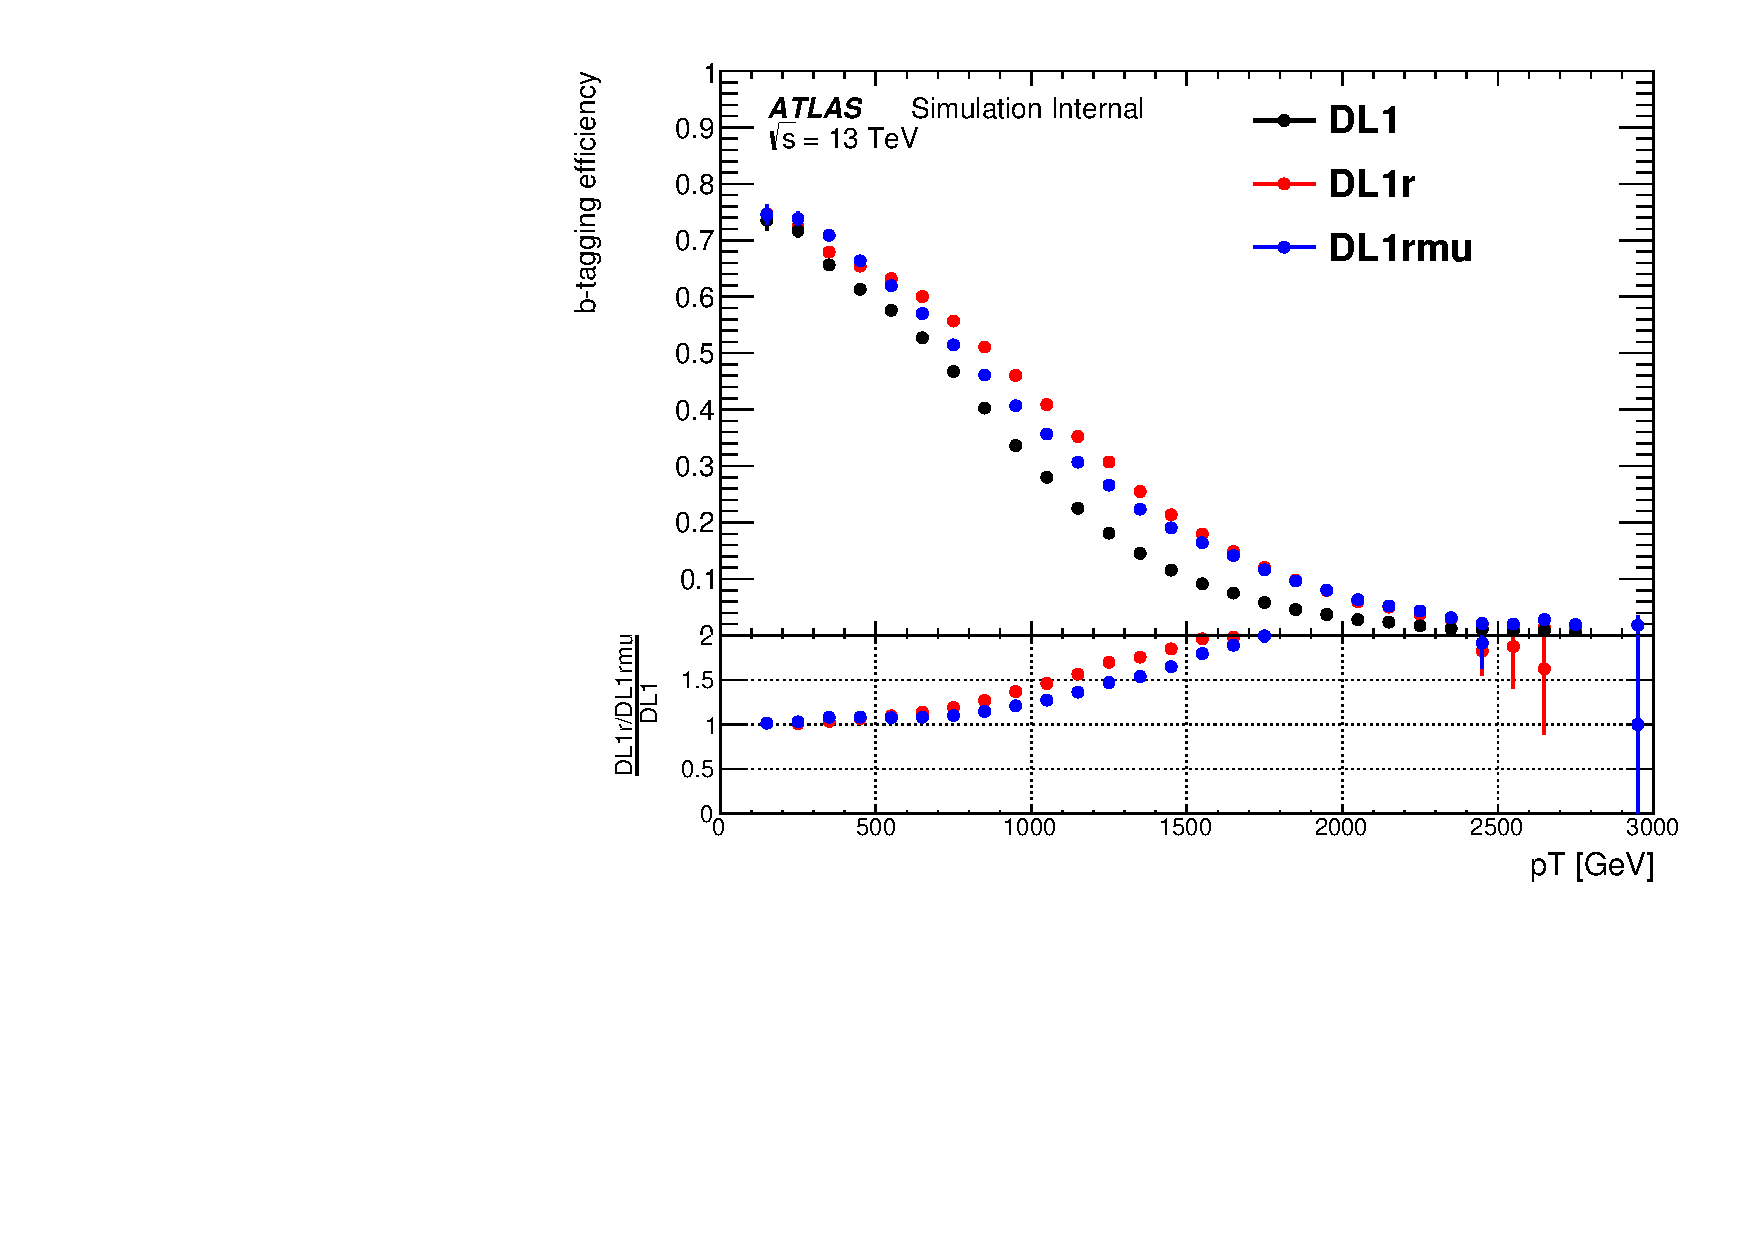
\includegraphics[width=0.9\textwidth]{figuresDijet/02-Selection/Zprime/Comparebtageff_Fix77.pdf}
  \caption{b-jet标定效率}
  \end{subfigure}
  \begin{subfigure}{.5\textwidth}
  \centering
   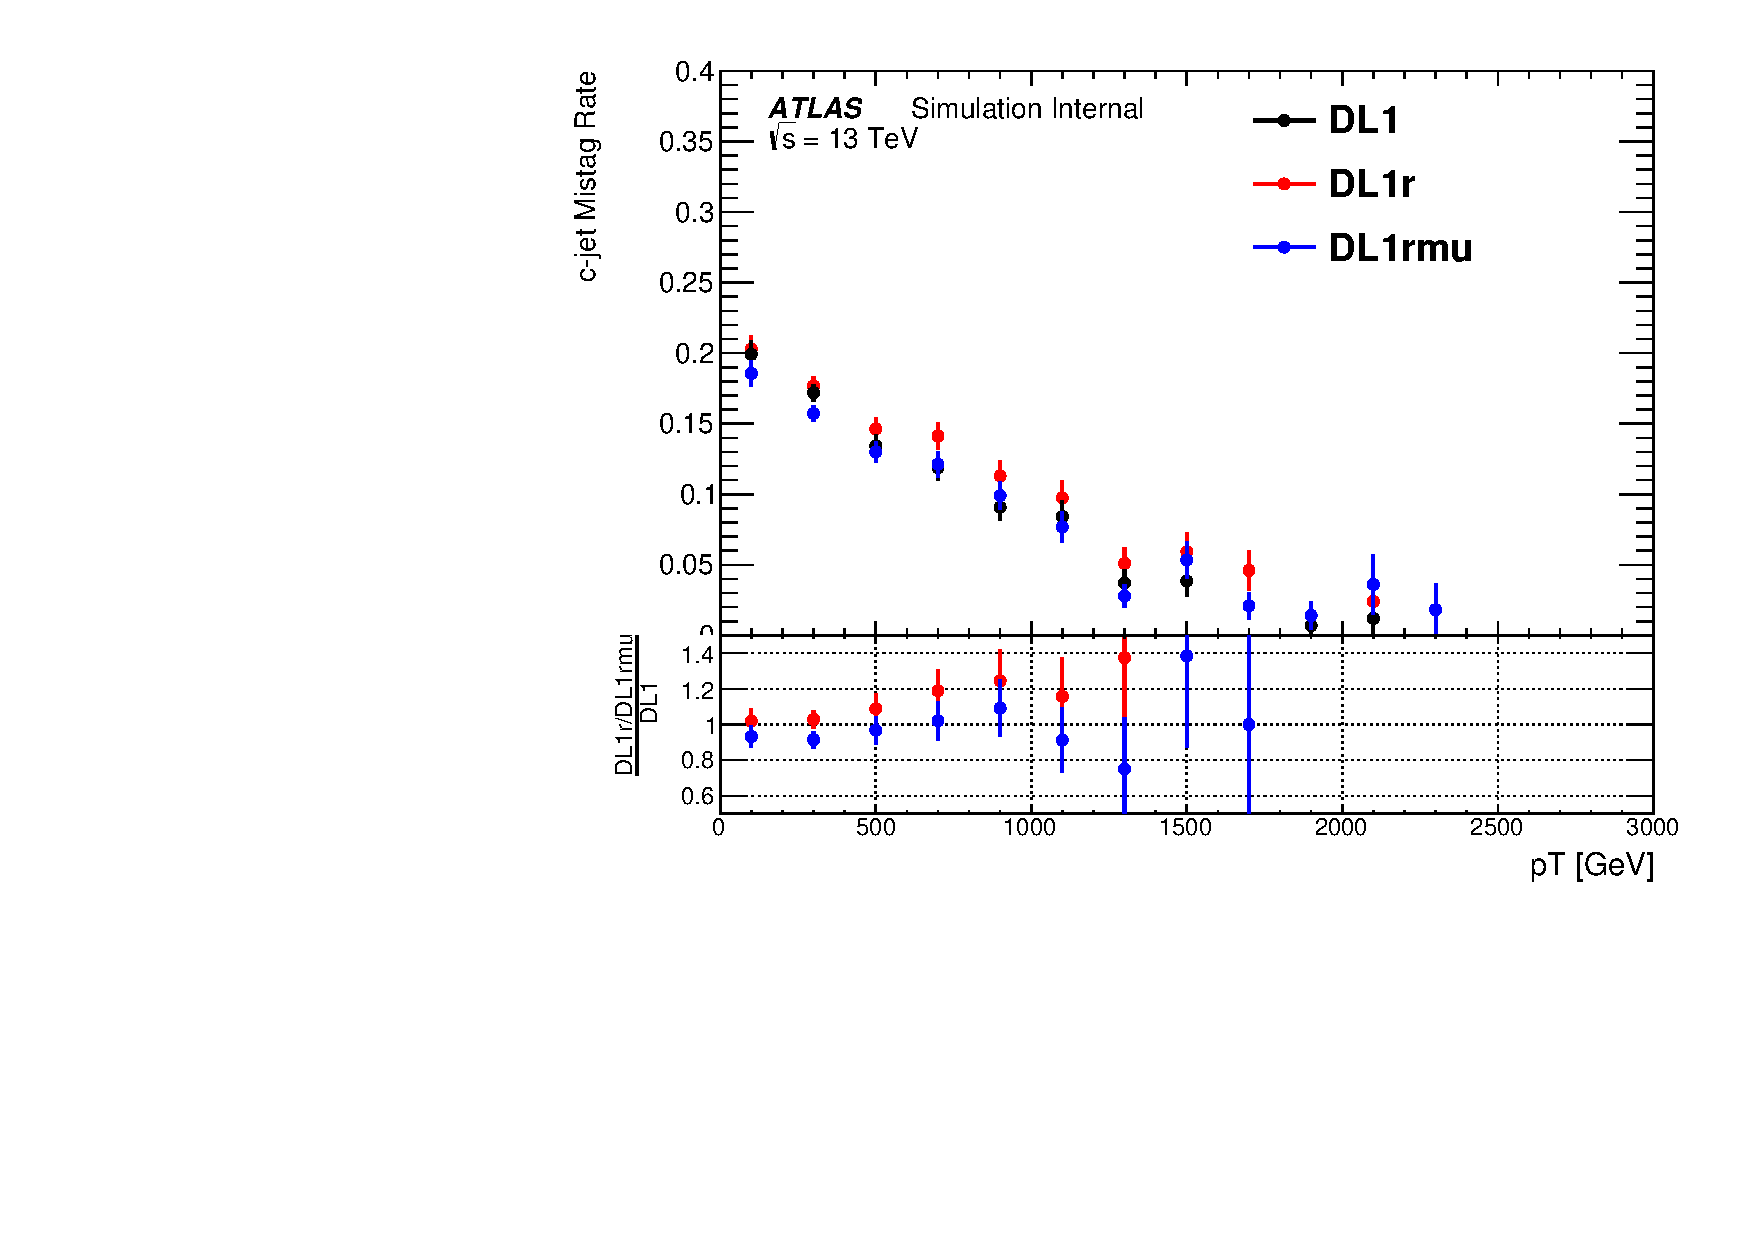
\includegraphics[width=0.9\textwidth]{figuresDijet/02-Selection/Zprime/Comparectageff_Fix77.pdf}
  \caption{c-jet误判率}
  \end{subfigure}
\newline 
  \begin{subfigure}{.99\textwidth}
  \centering
   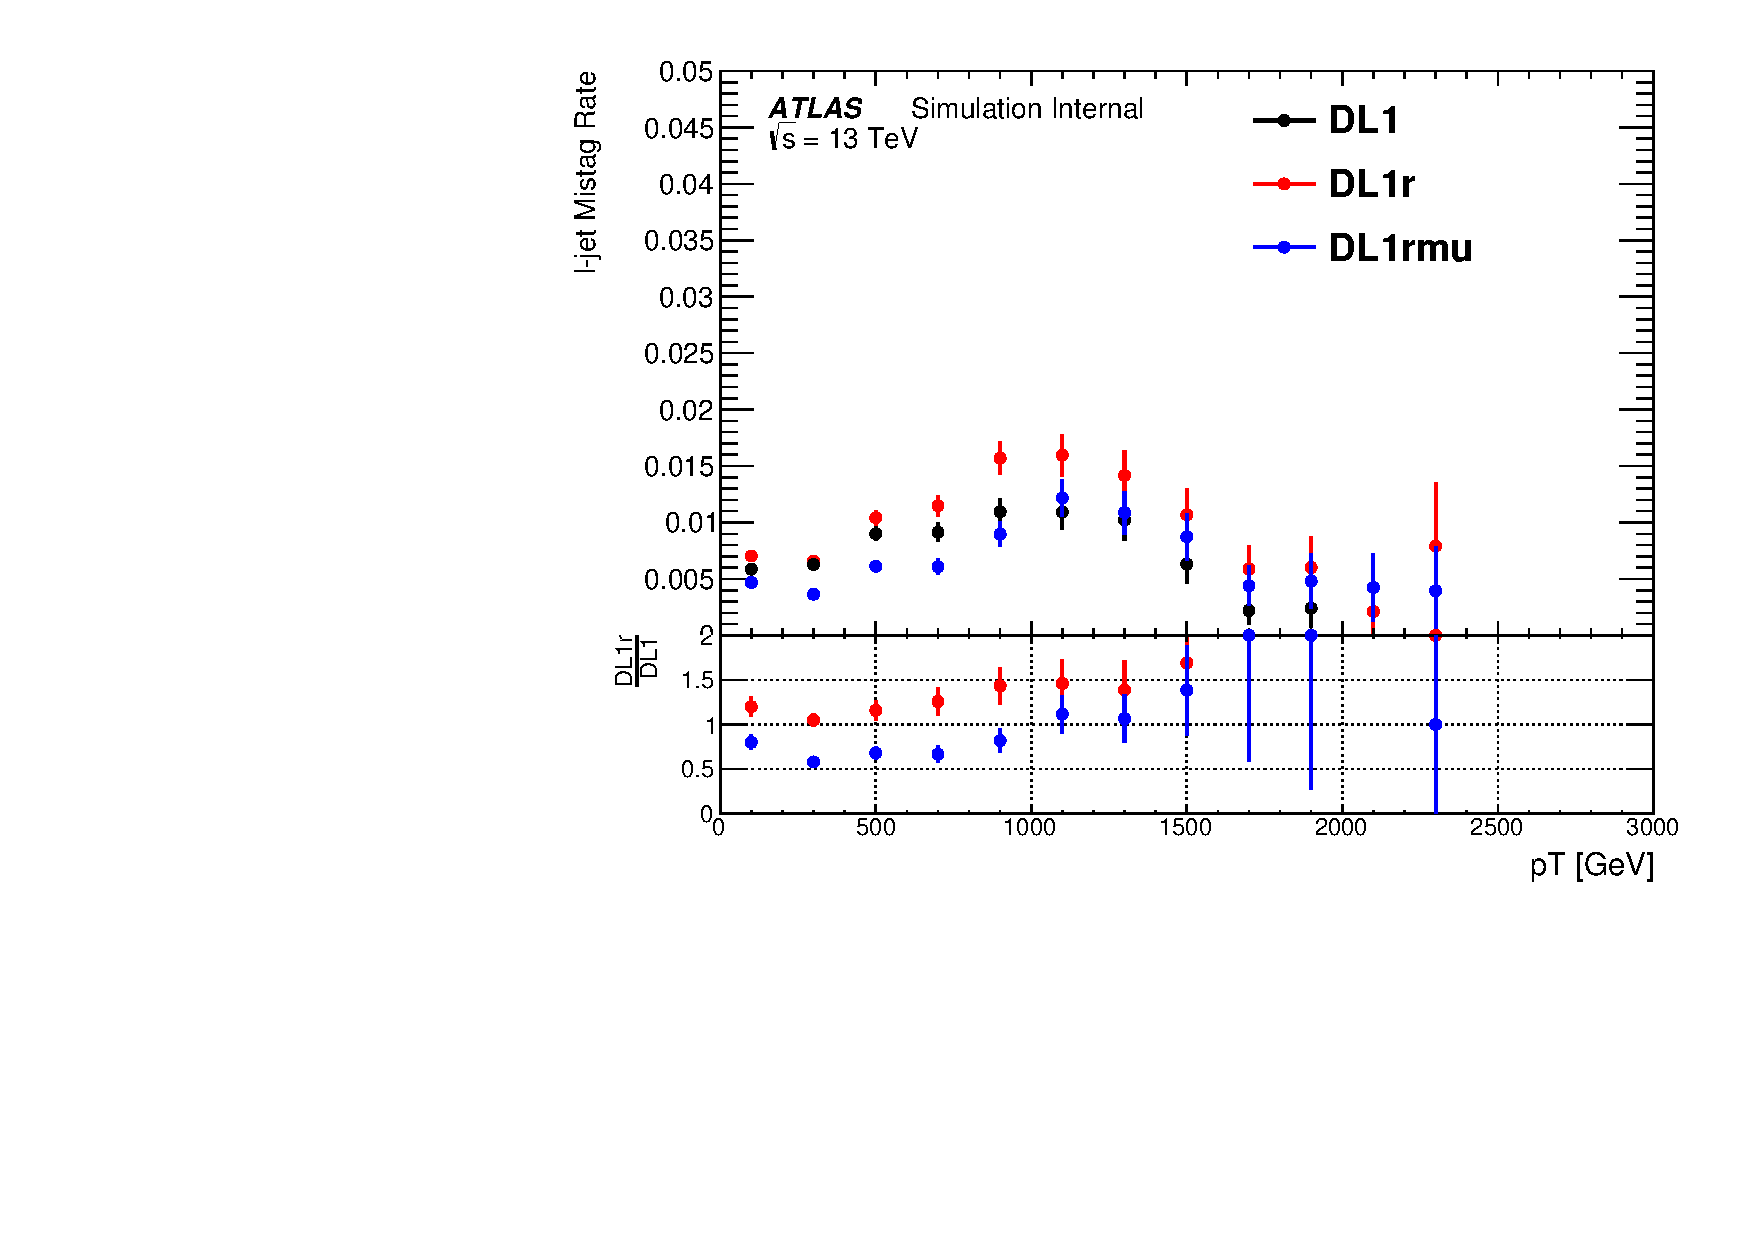
\includegraphics[width=0.5\textwidth]{figuresDijet/02-Selection/Zprime/Compareltageff_Fix77.pdf}
  \caption{light-jet误判率}
  \end{subfigure}
\caption{
在b-jet标定效率为77\%的工作点下,三种算法在DM $Z\prime\rightarrow b\bar{b}$信号中的b-jet标定效率、c-jet误判率和light-jet误判率随着jet横动量的变化关系。
}
\label{fig:btagperf_zprime_fix77}
\end{figure}



\begin{figure}[!thbp]
  \begin{subfigure}{.5\textwidth}
  \centering
  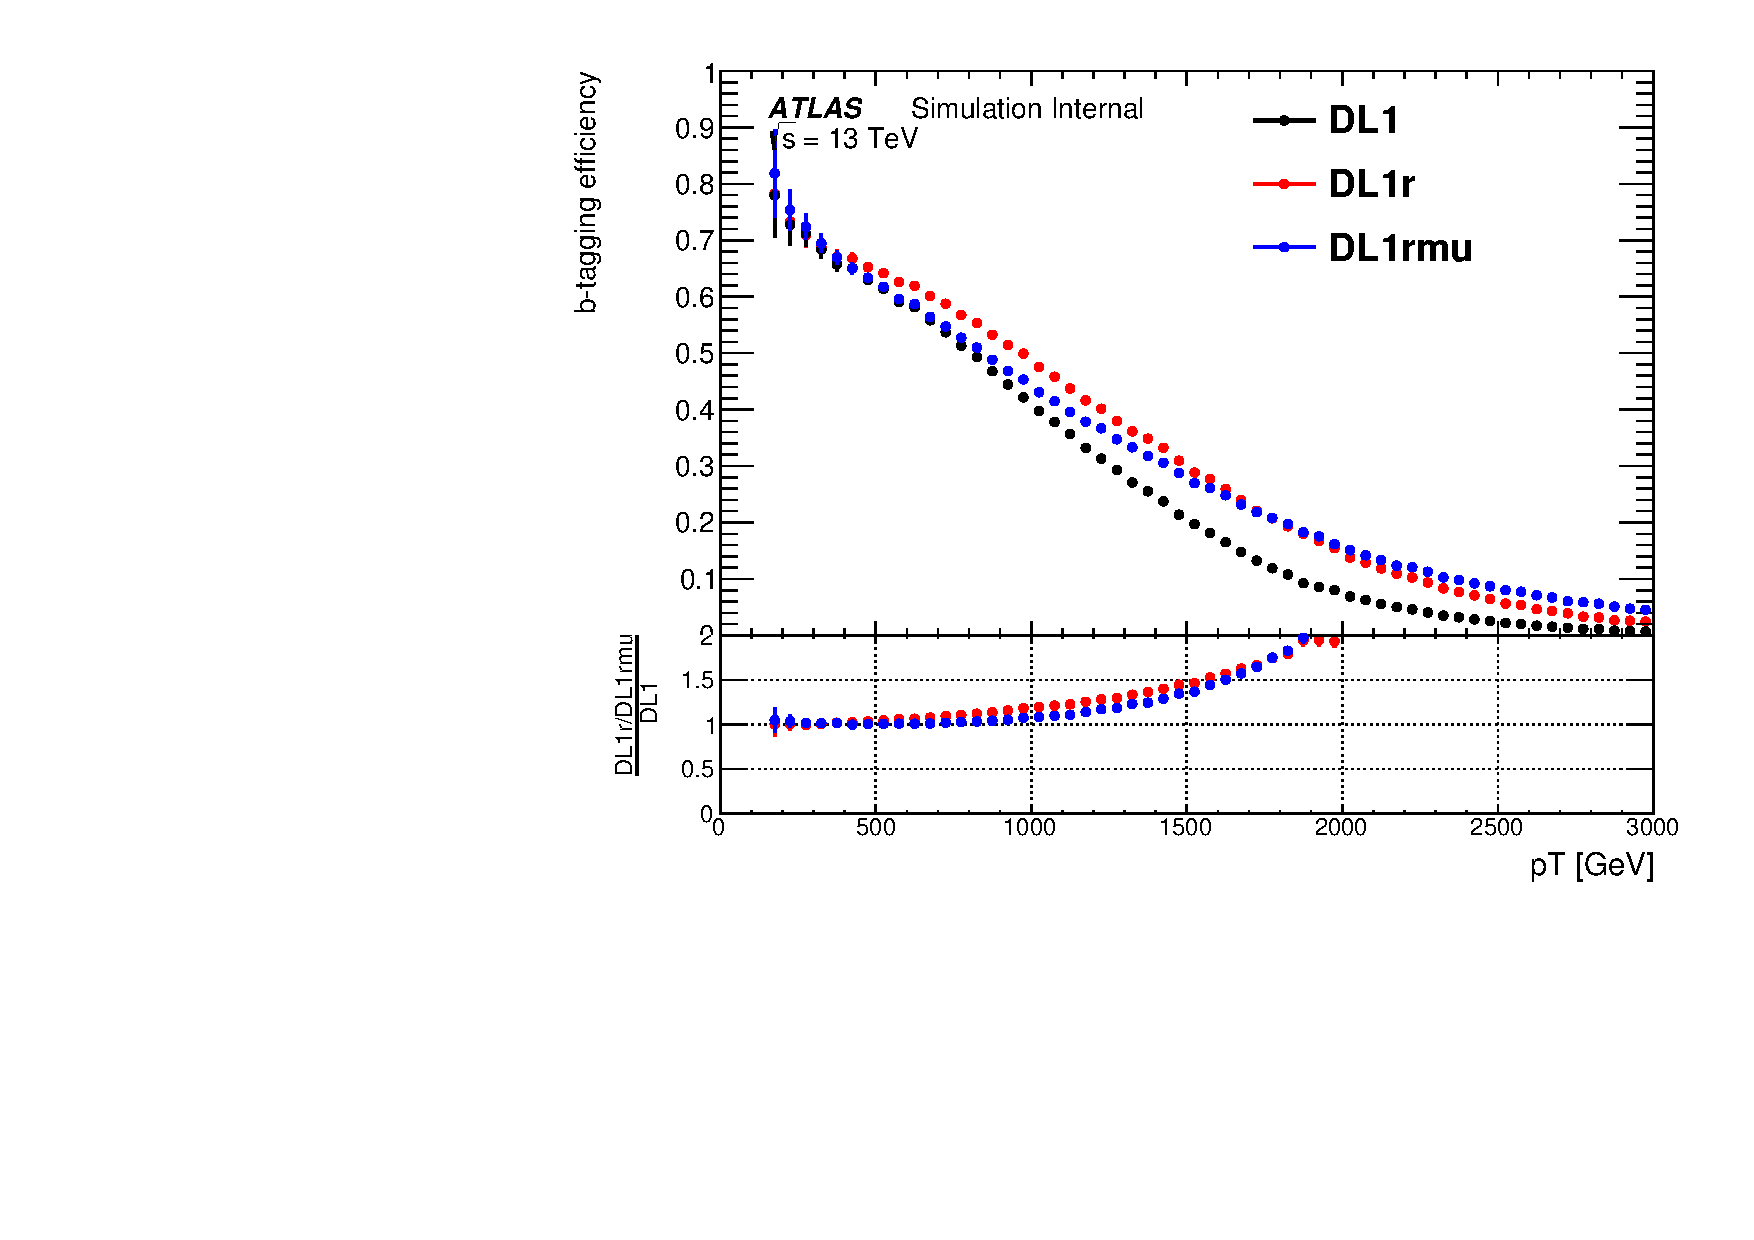
\includegraphics[width=0.9\textwidth]{figuresDijet/02-Selection/QCD/Comparebtageff_Fix77.pdf}
  \caption{b-jet标定效率}
  \end{subfigure}
  \begin{subfigure}{.5\textwidth}
  \centering
   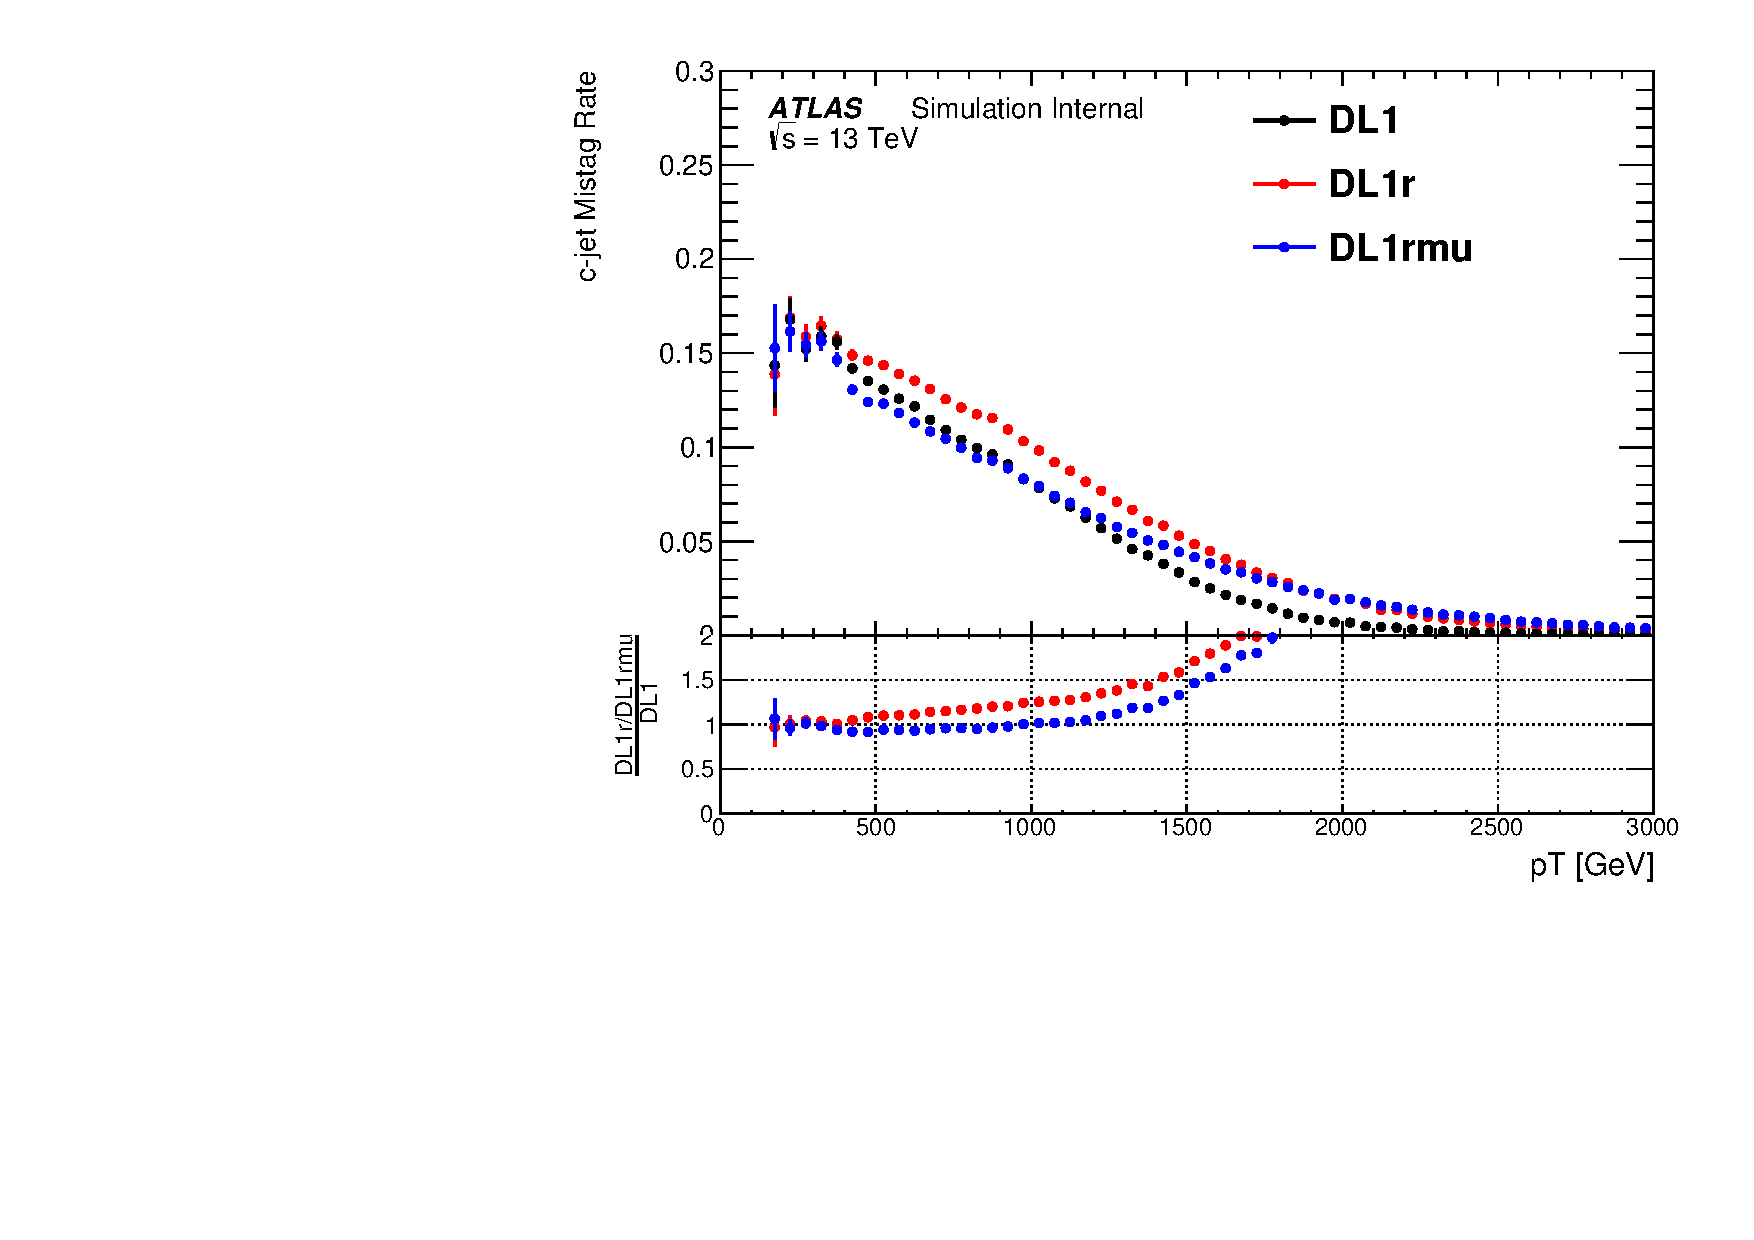
\includegraphics[width=0.9\textwidth]{figuresDijet/02-Selection/QCD/Comparectageff_Fix77.pdf}
  \caption{c-jet误判率}
  \end{subfigure}
\newline 
  \begin{subfigure}{.99\textwidth}
  \centering
  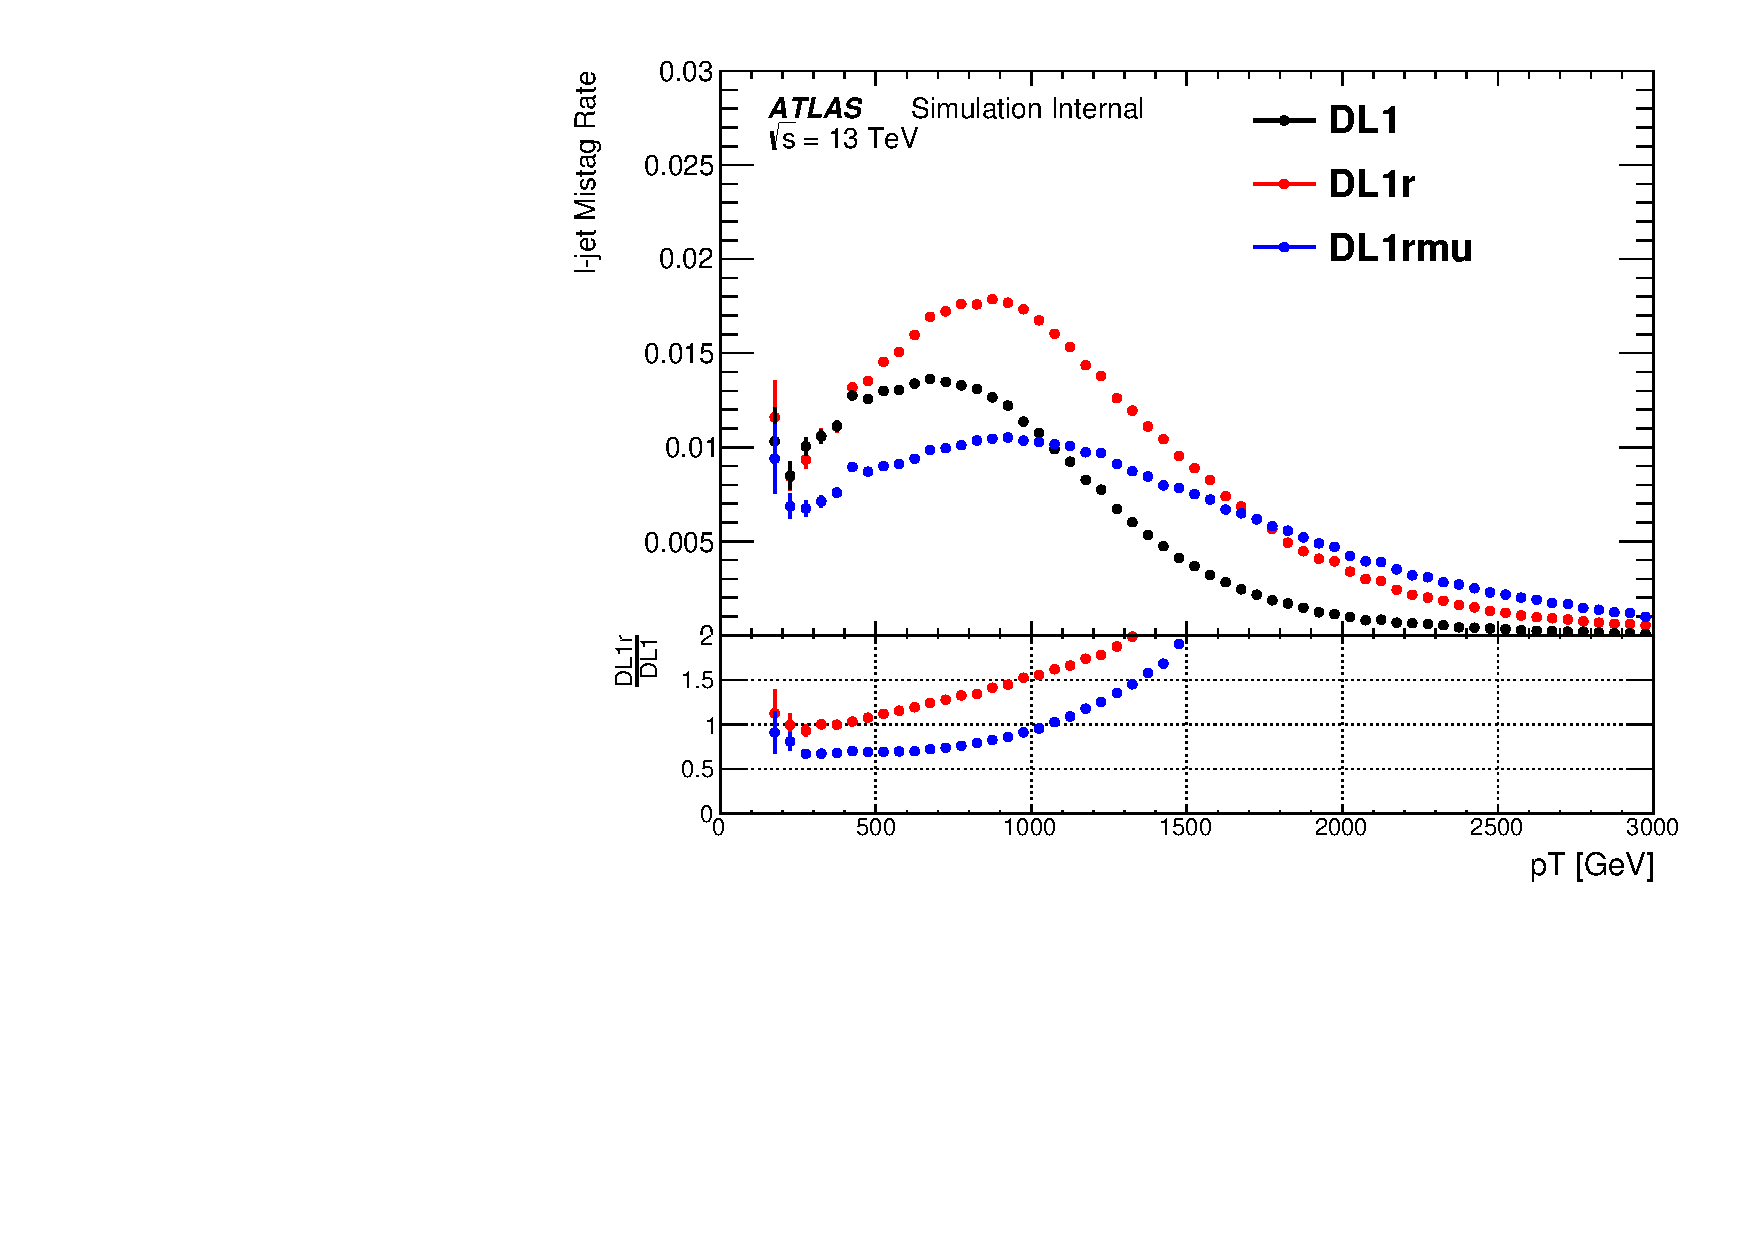
\includegraphics[width=0.5\textwidth]{figuresDijet/02-Selection/QCD/Compareltageff_Fix77.pdf}
  \caption{light-jet误判率}
  \end{subfigure}
\caption{
在b-jet标定效率为77\%的工作点下,三种算法在QCD本底中的b-jet标定效率、c-jet误判率和light-jet误判率随着jet横动量的变化关系。
}
\label{fig:btagperf_qcd_fix77}
\end{figure}


特别的,图~\ref{fig:btag2D_fix77}~展示了DM $Z\prime\rightarrow b\bar{b}$信号和QCD本底中DL1r算法在77\%的工作点下b-jet标定效率与$p_{T}$-$\eta$的二维依赖关系。

\begin{figure}[!thbp]
  \begin{subfigure}{.5\textwidth}
  \centering
  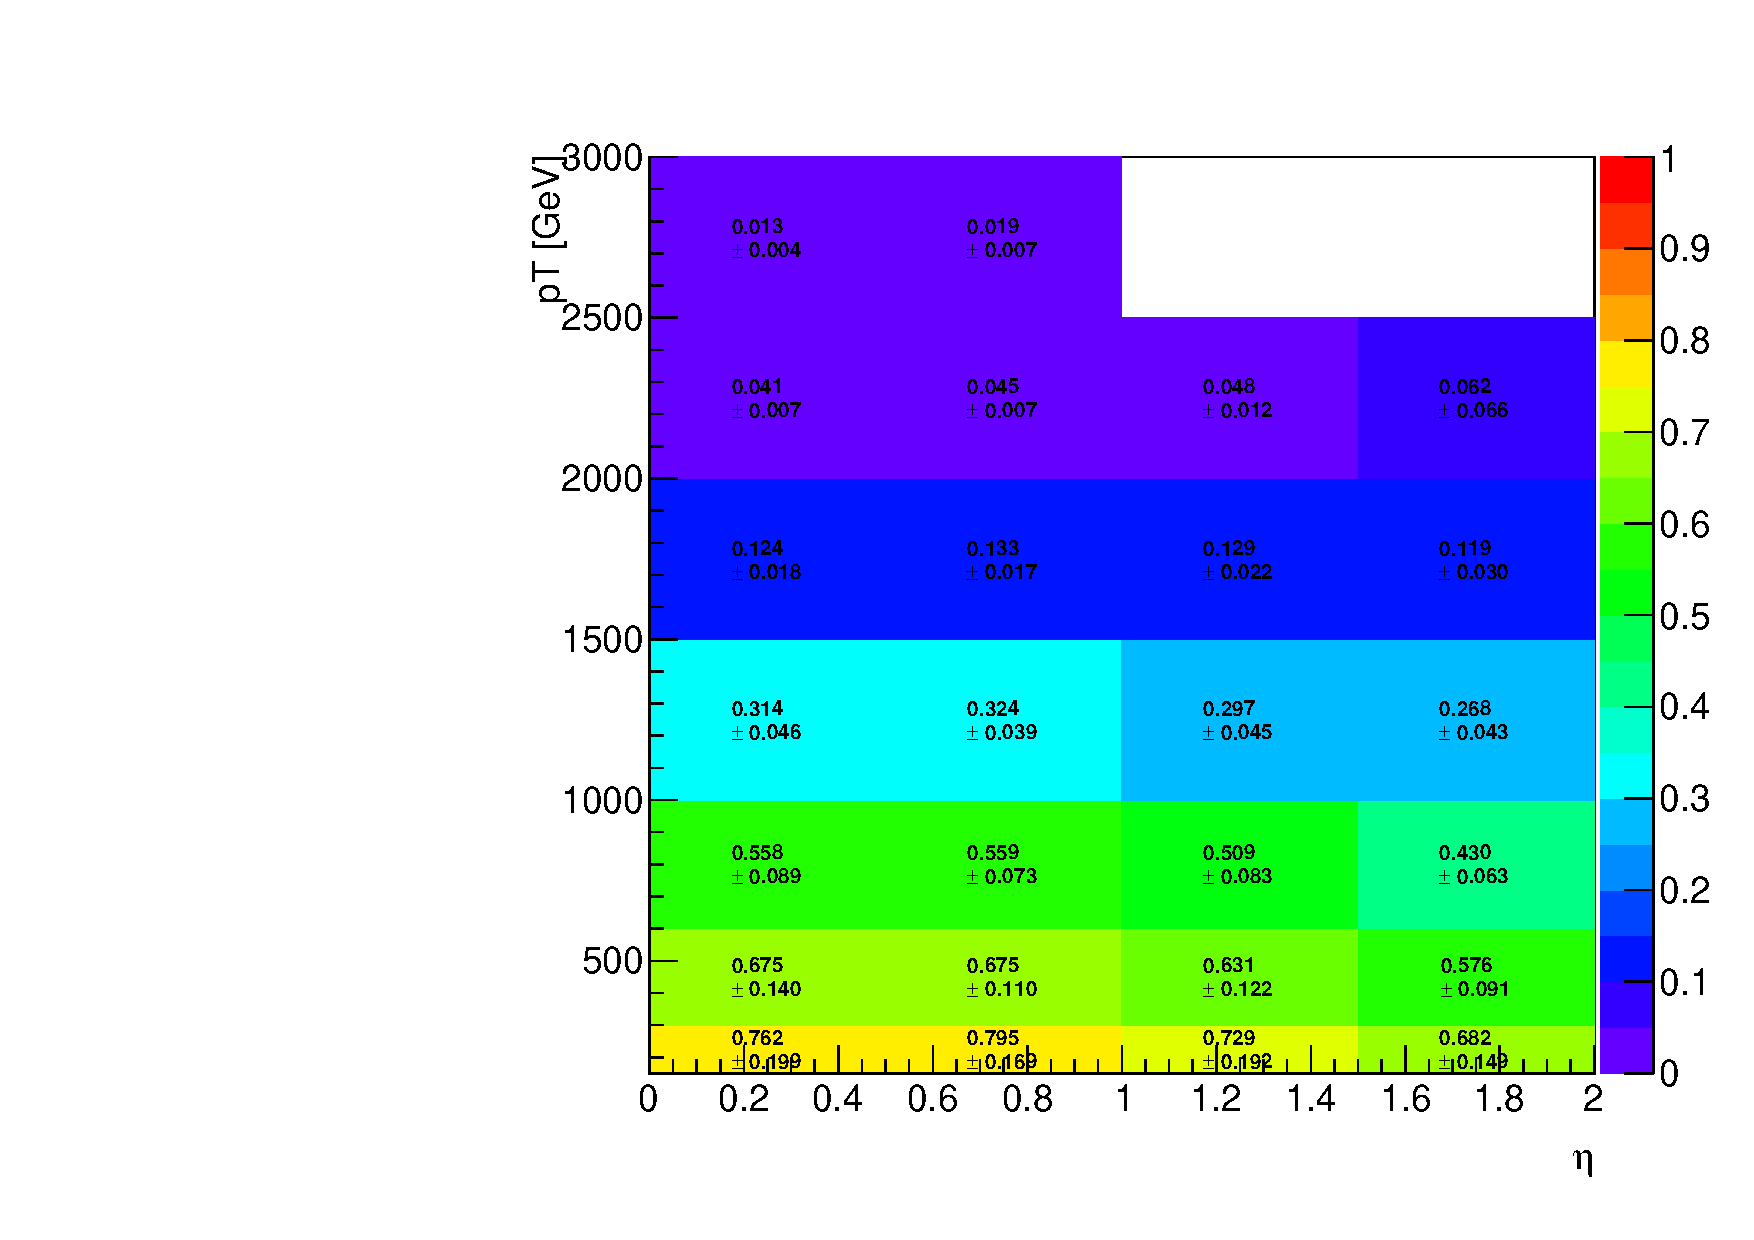
\includegraphics[width=0.9\textwidth]{figuresDijet/02-Selection/Btag_pteta2D_Fix77_DMZprime.pdf}
  \caption{DM $Z\prime \rightarrow  b\bar{b}$ 信号}
  \end{subfigure}
  \begin{subfigure}{.5\textwidth}
  \centering
  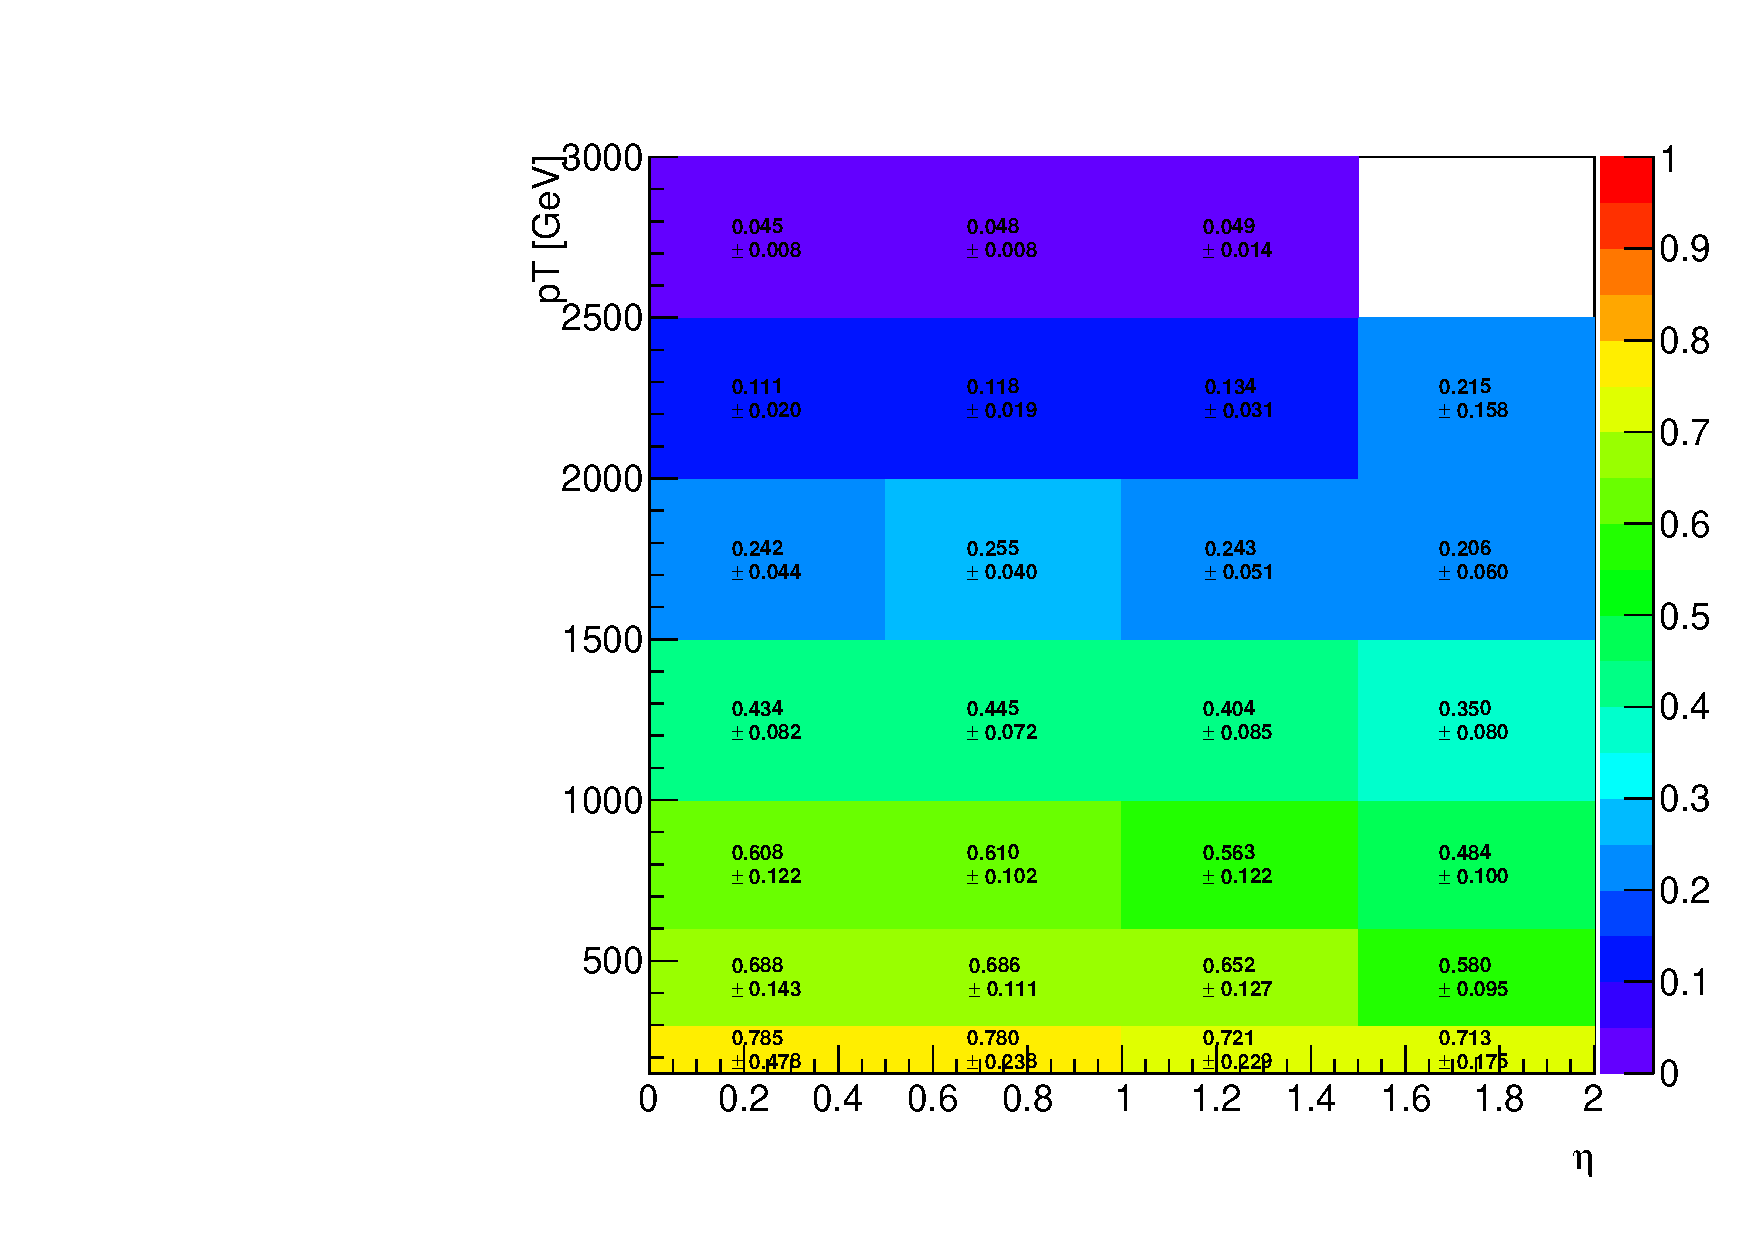
\includegraphics[width=0.9\textwidth]{figuresDijet/02-Selection/Btag_pteta_2D_Fix77_QCD.pdf}
  \caption{QCD本底}
  \end{subfigure}
\caption{
DM $Z\prime\rightarrow b\bar{b}$信号和QCD本底中DL1r算法在77\%的工作点下b-jet标定效率与$p_{T}$-$\eta$的二维依赖关系。
}
 \label{fig:btag2D_fix77}
\end{figure}



随后在对MC样本应用完整的事例筛选条件之后,对被选中的DL1r算法在选中的77\%的工作点下的性能进行了研究。
图~\ref{fig:beff}~ 所示为来自1b和2b信号区中各个信号的结果。
由于b-jet标定效率会随着jet横动量的增加而减小,因此图示效率随着$m_{jj}$的增大而减小。
在1b信号区中,衰变末态包含两个b-jet的$Z'$信号的b-jet标定效率比$b^*$信号的高。
在高质量区间,因为由$b^*$衰变而来的胶子更有可能衰变成$b\overline{b}$对,所以$b^*$信号的b-jet效率效率会得到相对加强从而接近$Z'$信号的效率。 

\begin{figure}[htbp]
  \centering
  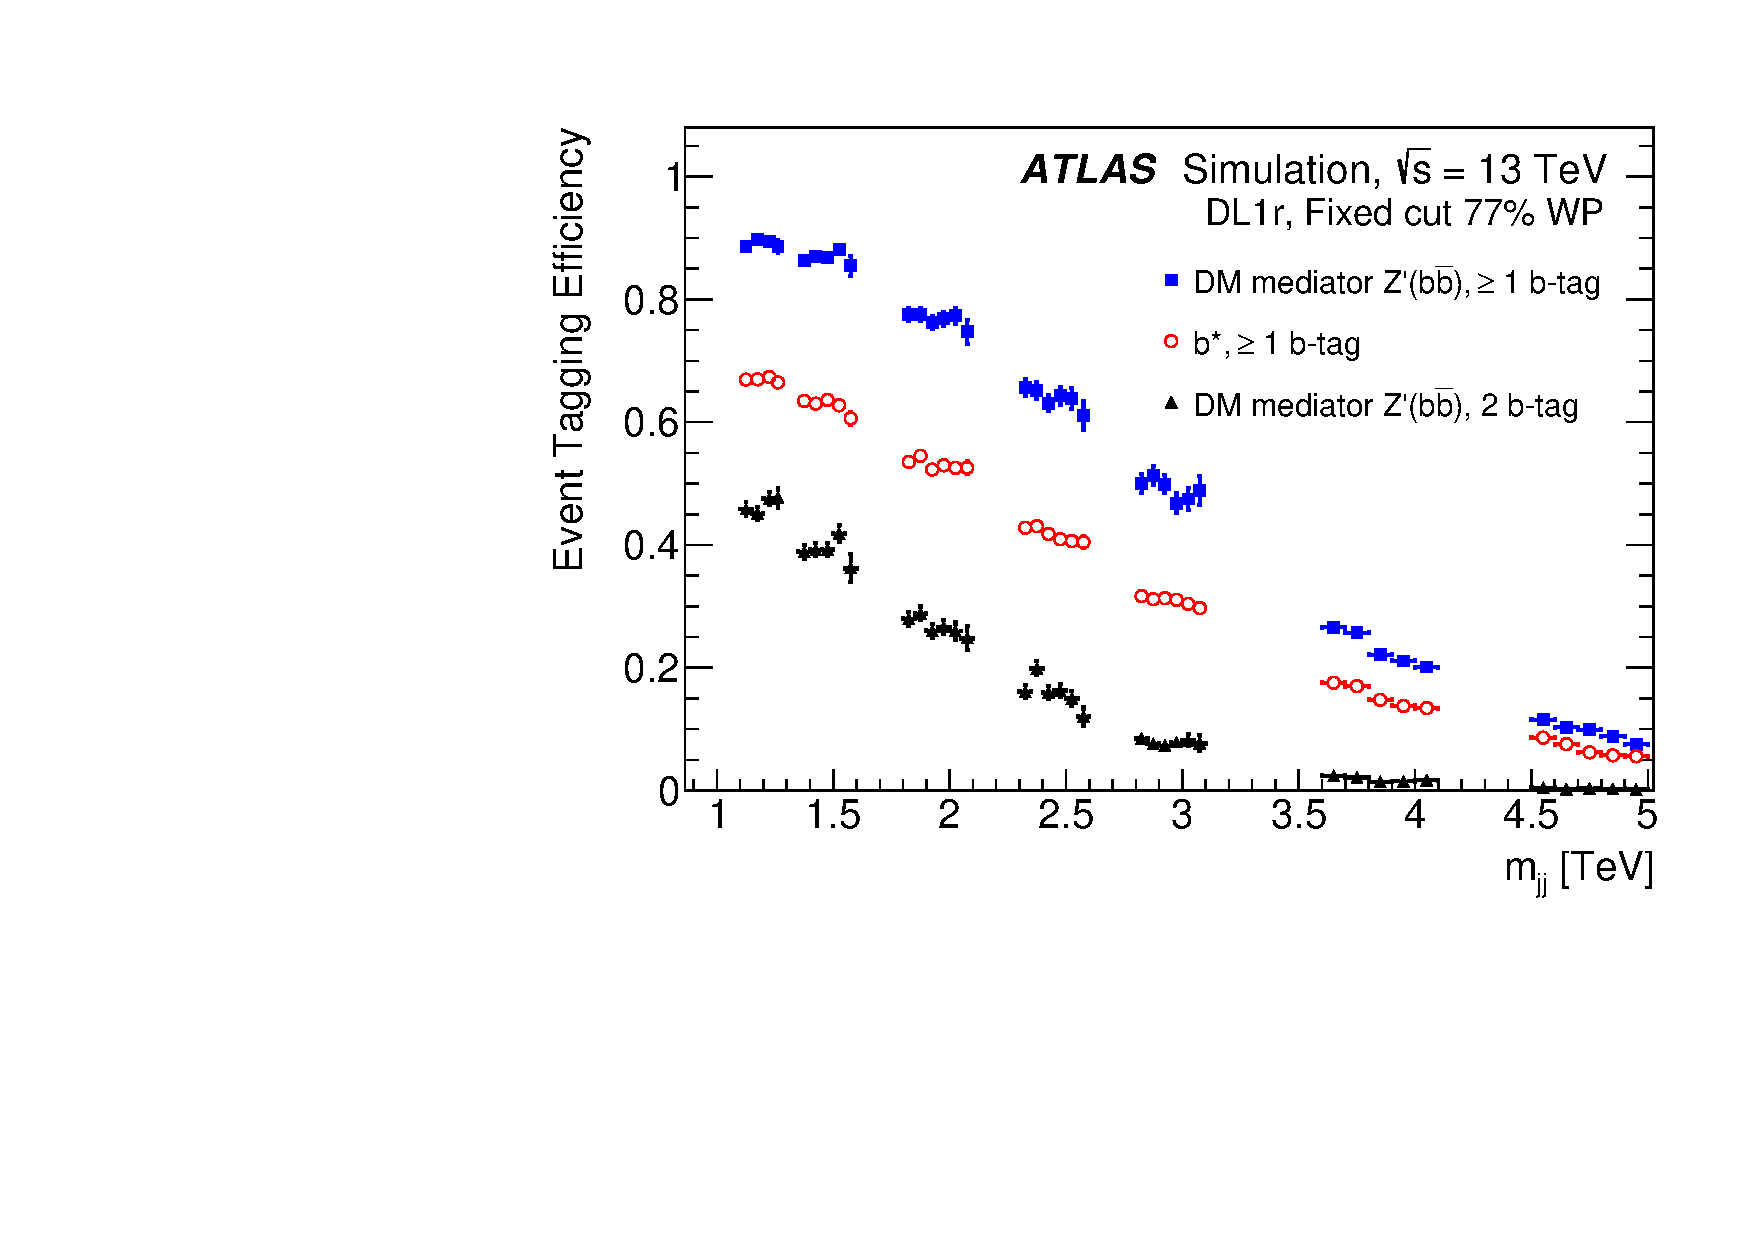
\includegraphics[width=0.75\textwidth]{figs/fig_02.pdf}
  \caption{在1b和2b信号区,DL1r标定算法在77\%的工作点下对不同信号的标定效率。}
  \label{fig:beff}
\end{figure}


\subsection{算法校准}
\label{sec:DijetBtagging4}

为了补偿b-jet标定效率在数据和MC中的差异,使用似然方法(Likelihood-based)引入了依赖于jet横动量的校准因子(Scale factor),并将它作用到MC上面~\cite{FTAG-2018-01}。
鉴于数据中b-jets的数量在$p_{T}>400GeV$时极少,通过在模拟中变化那些会影响b-jet标定性能的基本量来评估额外的误差,
然后为了在此分析中将校准因子的有效性扩展到更高的横动量区间,会将得到的b-jet标定效率差值和标准(nominal)的效率用来构建外推误差,
由此得到的DL1r标定算法在标定效率为$77\%$的工作点下的校准因子与jet横动量的关系如图~\ref{fig:SF}~所示。



\begin{figure}[thbp]
  \centering
  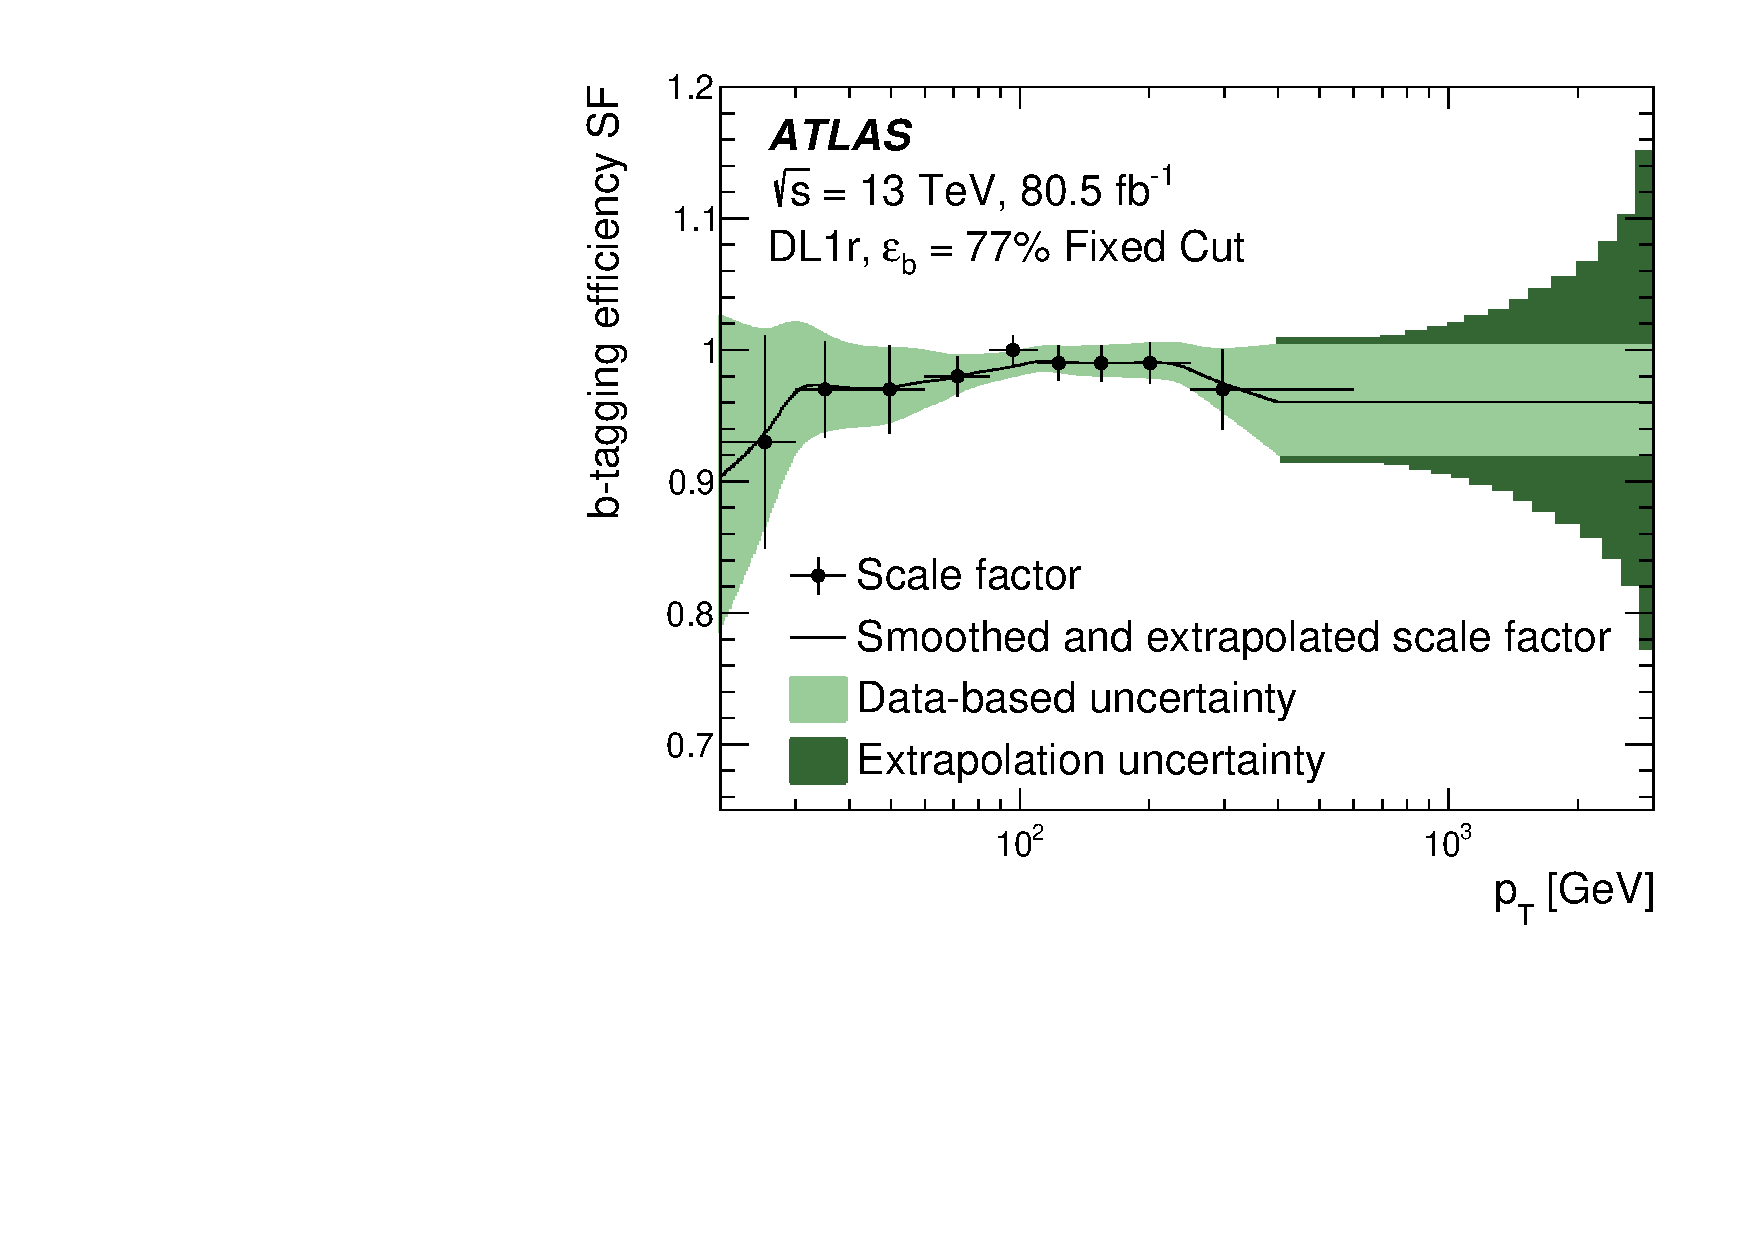
\includegraphics[width=0.75\textwidth]{figs/fig_01.pdf}
  \caption{  DL1r标定算法在标定效率为$77\%$的工作点下的校准因子随着jet横动量的变化关系。 }
  \label{fig:SF}
\end{figure}




\section{本底估计和新物理搜索}
\label{sec:DijetMjj}


\subsection{本底估计}
\label{sec:DijetMjj1}

标准模型所预言的dijet末态事例主要来自QCD过程,
而QCD预言的dijet末态事例的不变质量谱是平滑下降的,
因此可以用一个解析函数拟合来自实际数据的dijet末态事例的不变质量谱$m_{jj}$来确定来自QCD过程的本底~\cite{UA3},
以往的研究~\cite{ATLASDijet1,ATLASDijet2,ATLASDijet5}发现下列形式的参数函数:
\begin{equation}
\label{eq:Mjj1}
f(x)=p_1(1-x)^{p_2}x^{p_3+p_4\ln x}
\end{equation}
可以很好的描述来自领头阶和次领头阶QCD~MC样本所预言的dijet末态事例的不变质量谱,
其中$x= m_{jj}/\sqrt{s}$,$p_{1,2,3,4}$是四个拟合参数。
随着$Run\_2$计划中数据量的总积分亮度显著增加,
真实数据中dijet末态事例的不变质量谱$m_{jj}$统计量也会明显增加,
为了防止式~\ref{eq:Mjj1}~中参数函数对数据拟合失败,
我们使用滑动窗口拟合方法(the sliding-window fitting method)
%~\cite{EXOT-2016-21}
来代替全局拟合~\cite{ATLASDijet8}。

滑动窗口拟合方法是一种通过移动拟合中心依次在较小的$m_{jj}$范围内局部拟合的方法,
如图~\ref{fig:Mjj1}~所示,将$m_{jj}$低质量区的一个bin作为窗口中心,
然后围绕窗口中心,以左右bin数目为单位选择一个的窗口大小固定的窗口,
并在窗口内进行拟合,拟合完成之后,窗口中心向右滑动一个bin,
然后重新选择窗口进行拟合,直到拟合完成。
在这个分析当中,我们使用的窗口大小为48个bin,这个窗口大小足以完全覆盖我们要搜索的信号,
为了防止边缘效应,第一个bin和最后一个bin都不用做窗口中心,
且同时保证第一个窗口和最后一个窗口大小都能覆盖我们要搜索的信号。
%第一个窗口中心是$m_{jj}$中第24个bin,而最后一个窗口中心是$m_{jj}$中倒数第24个bin。
$m_{jj}$上每个bin的本底是通过对以该bin为窗口中心的窗口进行拟合得到的,
对于高质量区的bin和低质量区的bin,
我们将第一个窗口的低质量区bin的拟合结果和最后一个窗口的高质量区bin的拟合结果作为本底,
%对于前24个bin和最后24个bin,
%将第一个窗口的前24个bin的拟合结果和最后一个窗口后24个bin的拟合结果作为本底,
这样合并在一起构成了非参数化的全局$m_{jj}$本底。
如果全局的$\chi^2$~p-value~\cite{CHI2}大于0.05,则我们认为这种拟合方法对QCD本底的建模是合适的。

\begin{figure}[thbp]
  \centering
  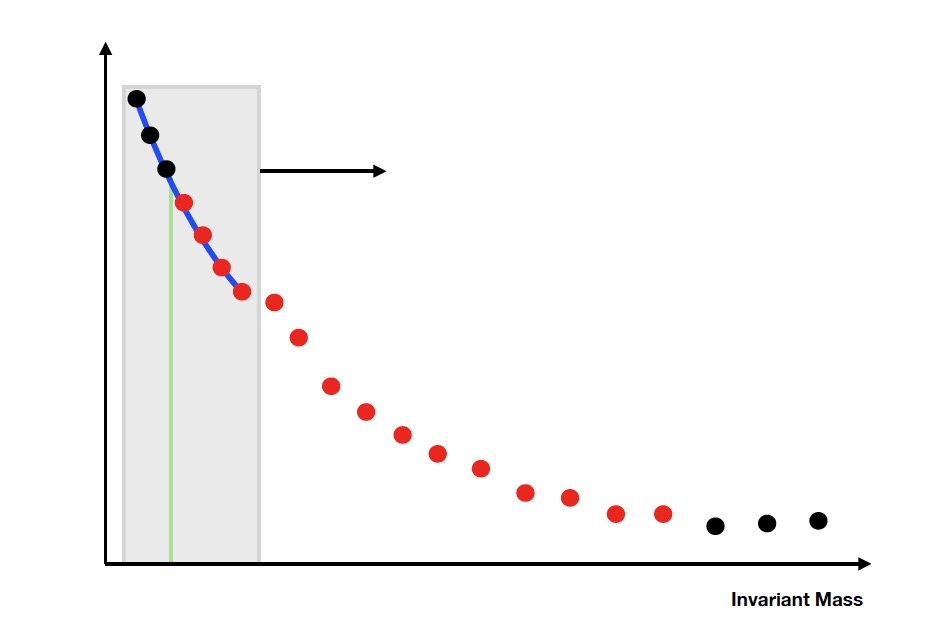
\includegraphics[width=0.75\textwidth]{figuresDijet/Mjj1.jpg}
  \caption{ 滑动窗口拟合方法示意图。途中绿色的垂线表示窗口中心,灰色框表示选中的窗口。  }
  \label{fig:Mjj1}
\end{figure}


\subsection{新物理搜索}
\label{sec:DijetMjj2}


在确定本底之后,实际数据中dijet末态事例的不变质量谱$m_{jj}$相对于本底的
局部突出的统计显著性是由\textsc{BumpHunter}算法~\cite{Aaltonen:2008vt,Choudalakis:2011bh}定量描述的。
\textsc{BumpHunter}计算了分bin的$m_{jj}$分布中质量连续的最突出的局部小段的统计显著性。

小段的宽度可以由$m_{jj}$分布的两个bin宽变化到整个$m_{jj}$分布长度的一半,
对于每个扫描到的小段,
\textsc{BumpHunter}算法首先会利用泊松随机涨落计算数据和本底之间差异的显著性,
以局部p-value来表征:
\begin{equation} 
\label{eq:Bump1}
p-value=
\begin{cases}
      \sum_{n=D}^{\infty} \frac{B^n e^{-B}}{n!}, \quad \text{for D \geq B}\\
      \sum_{n=0}^D \frac{B^n e^{-B}}{n!}, \quad \text{for D < B }
    \end{cases}
\end{equation}
其中D是小段中的数据事例数,B是小段中本底的事例数。
随后利用局部p-value构造一个统计检验量t:
\begin{equation} 
\label{eq:Bump2}
t=-log(p-value_{min})
\end{equation}
其中$p-value_{min}$是搜索中考虑到的所有局部小段的局部p-value值中最小的那个值,
这个统计检验量t用于评估分布中最突出的局部小段的全局p-value。
局部p-value考虑的是特定小段的显著性,
而与局部p-value不同的是,全局p-value考虑的是分布中任意局部突出的显著性,
这也是“别处效应”的基本思想~\cite{lookelsewhere}。
%这里我们通过\textsc{BumpHunter}算法的p-value来评估该小段的显著性,
%\textsc{BumpHunter}算法p-value是通过执行一系列从本底估计得到的赝实验(pseudo-experiments)确定的。

由\textsc{BumpHunter}算法标记的数据中与本底偏离最显著的局部小段是通过这样一组bin来定义的,
由本底泊松涨落造成该组bin的出现的概率最小,即局部p-value最小。
而该小段的在整个分布中的显著性是通过全局p-value来评估的,记为\textsc{BumpHunter}算法p-value,
它的的含义是,在全本底假设的情况下,由于随机涨落产生的最突出的局部小段比所观测到的最突出的局部小段更加显著的概率,
我们用它来决定是否拒绝全本底假设。
通过在10000个由本底估计得到的赝实验(pseudo-experiments)上执行上述步骤,
可以得到统计检验量t的分布,然后可以计算出\textsc{BumpHunter}算法p-value。
在一个好的拟合当中,任何的局部突出都是由拟合出来的本底分布的涨落引起的。
这里也可以通过\textsc{BumpHunter}的来评估拟合质量,在决定滑动窗口拟合方法的窗口长度时,
如果对应的\textsc{BumpHunter}算法p-value值大于0.01,我们则认为这个拟合是可以被接受的,
没有显著的新物理信号。

除此之外,$m_{jj}$分布中每个bin上数据与本底之前差异的显著性也非常重要,
为了显示这些差异,我们使用了标准偏差中的显著性~\cite{ZVA}。
首先按式~\ref{eq:Bump1}~计算每个bin上的p-value,
这里D和B分别表示每个bin上的数据事例数和本底事例数。
这里计算出来的p-value跨越多个数量级,为了方便,将它转化为z-value,
z-value和p-value在表示显著性方面是等效的,
表示一个高斯分布在右侧的标准偏差,转化关系如下:
\begin{equation} 
\label{eq:Bump3}
p-value=\sum_{z-value}^{\infty} \frac{1}{\sqrt{2\pi}} e^{-\frac{x^2}{2}} dx
\end{equation}
这里仅z-value为正数的情况被考虑进来,
对应于p-value$\le 0.5$,其他情况的偏差都极小。 
随后根据bin中数据和本底的大小关系为z-value附加一个正负号,
当本底事例数大于数据事例数时,z-value取正号,
当本底事例数小于数据事例数时,z-value取负号。
z-value比较大就表明数据和本底之前存在显著的偏差,比如z-value$\geq 3$。

%在确定本底之后,实际数据中dijet末态事例的不变质量谱$m_{jj}$相对于本底的
%局部突出的统计显著性是由\textsc{BumpHunter}算法~\cite{Aaltonen:2008vt,Choudalakis:2011bh}定量描述的。
%\textsc{BumpHunter}计算了分bin的$m_{jj}$分布中质量连续的最突出的局部小段的统计显著性,
%其中小段的宽度由$m_{jj}$分布的两个bin宽变化到整个$m_{jj}$分布长度的一半,对于每个扫描到的小段,\textsc{BumpHunter}算法会计算数据和本底之间差异的显著性,
%数据中与本底偏离最显著的局部小段是通过这样一组bin来定义的,由本底泊松涨落造成该组bin的出现的概率最小。
%这里我们通过\textsc{BumpHunter}算法的p-value来评估该小段的显著性,
%它的的含义是,在全本底假设的情况下,由于随机涨落产生的最突出的局部小段比所观测到的最突出的局部小段更加显著的概率。
%在考虑别处效应~\cite{lookelsewhere}的情况下,它是通过执行一系列从本底估计得到的赝实验(pseudo-experiments)确定的。
%在一个好的拟合当中,任何的局部突出都是由拟合出来的本底分布的涨落引起的。
%这里也可以通过\textsc{BumpHunter}的来评估拟合质量,在决定滑动窗口拟合方法的窗口长度时,
%如果对应的\textsc{BumpHunter}算法的p-value值大于0.01,我们则认为这个拟合是可以被接受的,
%而且没有显著的新物理信号。

\subsection{有效性验证}
\label{sec:DijetMjj3}

在搜索实际的数据之前,
我们使用了多个数据驱动(data-driven)的$m_{jj}$本底来验证这种拟合本底策略的有效性。
在1b和2b信号区,由于QCD~MC样本的统计量低,我们使用ABCD方法来获取用于有效性验证的$m_{jj}$本底,
这种方法已经在以前的类似分析中得到成功应用~\cite{ATLASDijet9},
这里使用性能更好的DL1r标定算法在77\%的工作点下再次应用,
首先,根据事例中两个不相关的变量$|y^*|$和b-jet标定数目将数据分为四个区域:
\begin{itemize}
  \item 区域A:事例中两个领头阶jet满足$|y^*|>0.8$,且对于1b信号区,被标定的b-jet有一个,对于2b信号区,两个都被标定为b-jet;
  \item 区域B:事例中两个领头阶jet满足$|y^*|<0.8$,且对于1b信号区,被标定的b-jet有一个,对于2b信号区,两个都被标定为b-jet;
  \item 区域C:事例中两个领头阶jet满足$|y^*|>0.8$;
  \item 区域D:事例中两个领头阶jet满足$|y^*|<0.8$。
\end{itemize}
通过反转$|y^*|$的筛选条件,区域A和C中的信号残余可以忽略不计,
信号区即区域B中的数据可以通过以下式子推断:
\begin{equation}
\label{eq:Mjj2}
N_B=N_D	\epsilon
\end{equation}
其中$N_B$和$N_D$分别是区域B和区域D中相应事例数,
$\epsilon$是通过区域A和C得到的b-jet标定效率,
它主要和jet的$p_{T}$和$\eta$相关,
因此这里使用了二维效率映射,
映射关系是通过反转分析中$|y^*|$的筛选条件得到的。
按条件这里需要如下三个映射关系才能充分考虑到领头jet和次领头jet之间的关联性:
\begin{itemize}
  \item 要求事例中领头jet被DL1r标定为b-jet,同时对次领头jet没有标定要求。
 这种条件下由式~\ref{eq:Mjj2}~得到的映射关系记为$\epsilon_{j1}$。
   \item 要求事例中次领头jet被DL1r标定为b-jet,同时对领头jet没有标定要求。
 这种条件下由式~\ref{eq:Mjj2}~得到的映射关系记为$\epsilon_{j2}$。
   \item 要求事例中领头jet和次领头jet都被DL1r标定为b-jet。
 这种条件下由式~\ref{eq:Mjj2}~得到的映射关系记为$\epsilon_{j1j2}$。
\end{itemize}
图~\ref{fig:maps}~展示了这三个二维映射关系,
然后,1b信号区的映射关系由如下式子计算得到:
\begin{equation}
\label{eq:Mjj3}
\epsilon_{1b} = \epsilon_{j1} + \epsilon_{j2} - \epsilon_{j1} \epsilon_{j1j2}
\end{equation}
而2b信号区的映射关系由以下式子计算:
\begin{equation}
\label{eq:Mjj4}
\epsilon_{2b} = \epsilon_{j1}  \epsilon_{j1j2}
\end{equation}
由领头jet和次领头jet得到1b和2b记信号区的映射关系之后,
可以用这个映射关系来给区域D中相应$p_{T}$-$\eta$二维区间的事例赋予权重,
由此可以得到我们所估计的区域B也就是1b和2b信号区的$m_{jj}$本底。

\begin{figure}[!thbp]
  \begin{subfigure}{1\textwidth}
  \centering
  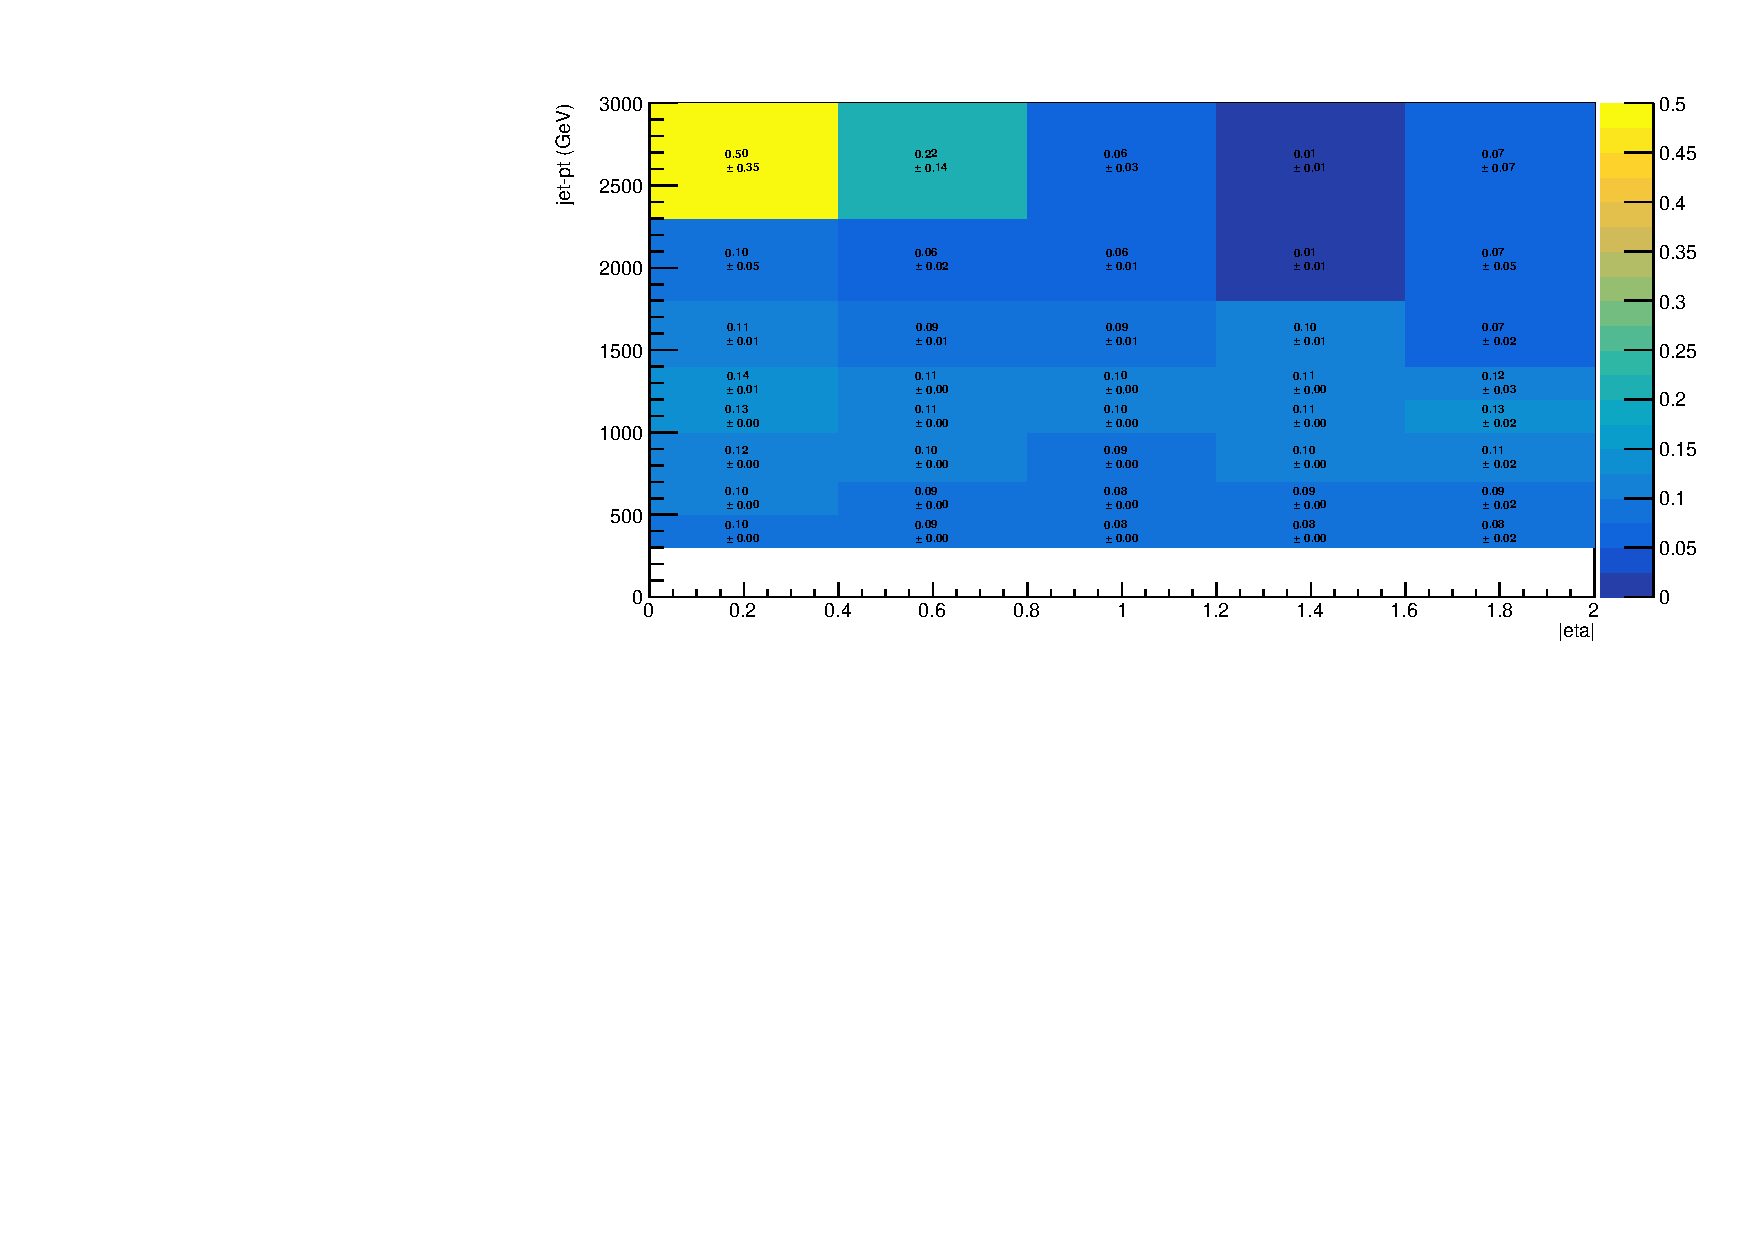
\includegraphics[width=0.75\textwidth]{figuresDijet/04-BackgroundEstimation/lead_map.pdf}
  \caption{$\epsilon_{j1}$}
  \end{subfigure}
  \begin{subfigure}{1\textwidth}
  \centering
  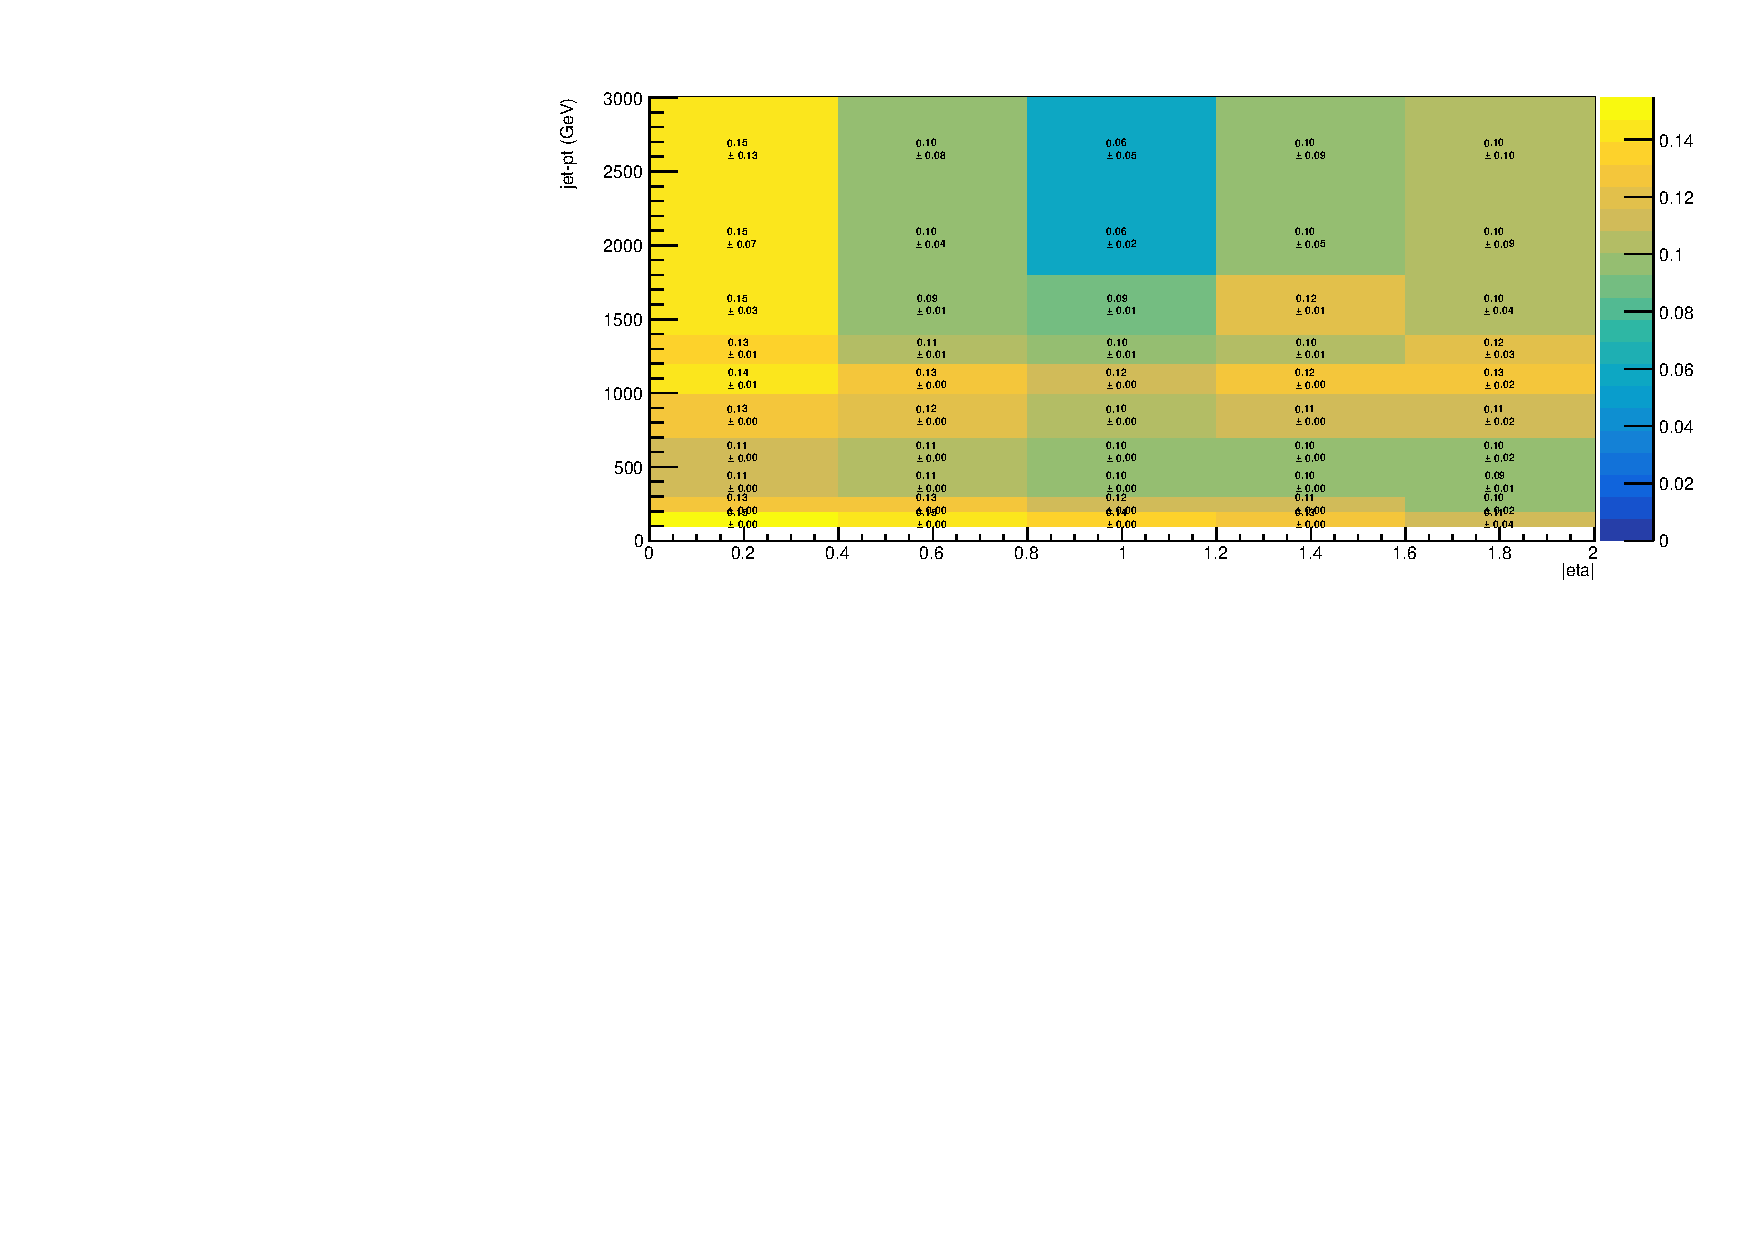
\includegraphics[width=0.75\textwidth]{figuresDijet/04-BackgroundEstimation/sublead_map.pdf}
  \caption{$\epsilon_{j2}$}
  \end{subfigure}
\newline 
  \begin{subfigure}{1\textwidth}
  \centering
  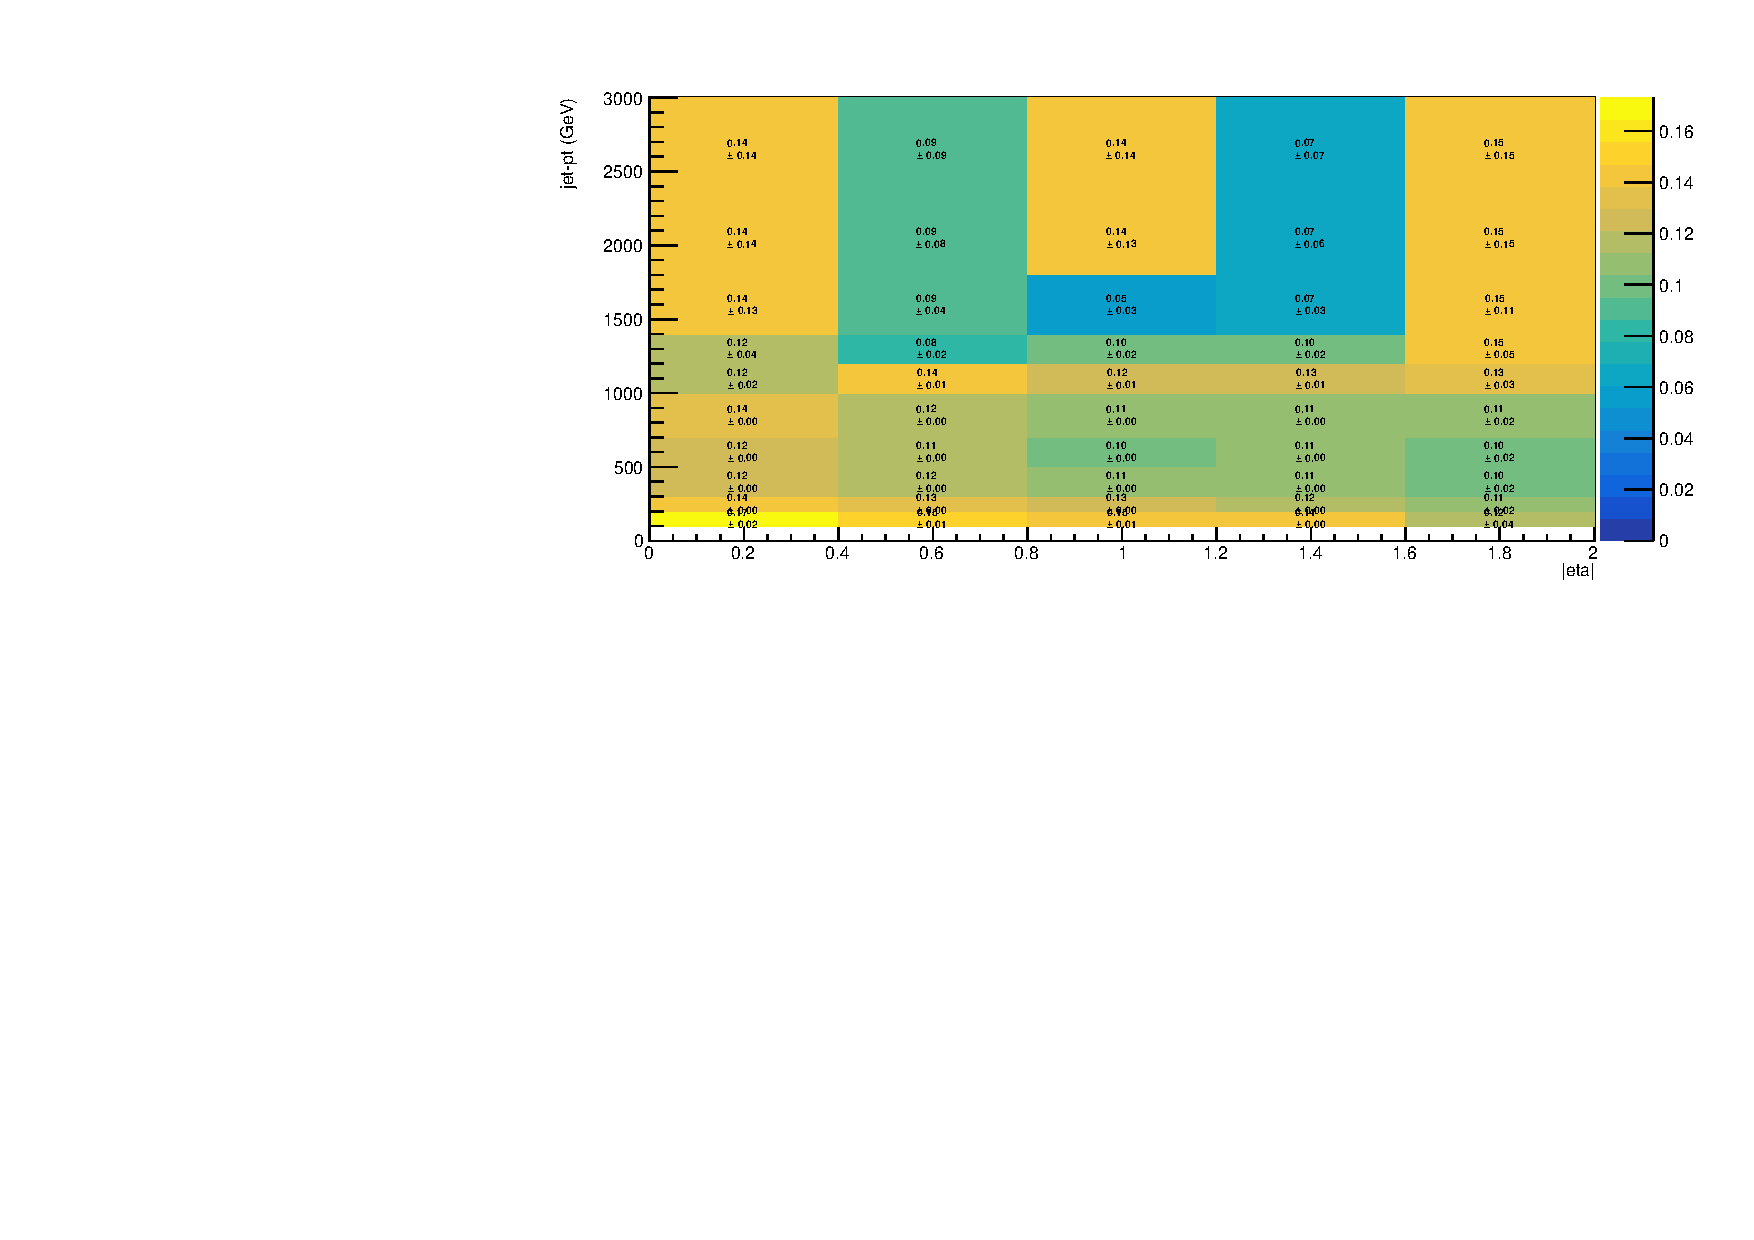
\includegraphics[width=0.75\textwidth]{figuresDijet/04-BackgroundEstimation/conditional_eff.pdf}
  \caption{$\epsilon_{j1j2}$}
  \end{subfigure}
  \caption{ABCD方法中三个效率映射关系。(a) $\epsilon_{j1}$;(b) $\epsilon_{j2}$;(c) $\epsilon_{j1j2}$。}
\label{fig:maps}
\end{figure}



为了验证ABCD方法,我们使用ATLAS在2016年收集的未发现显著的新物理信号的数据~\cite{ATLASDijet8,ATLASDijet9}中一小部分进行了测试,
如图~\ref{fig:validationABCD}~所示是用ABCD方法得到的信号区$m_{jj}$和实际数据中的$m_{jj}$的对比,
可以看到它们符合的非常一致,因此ABCD方法得到验证。

\begin{figure}[!ht]
	\centering
	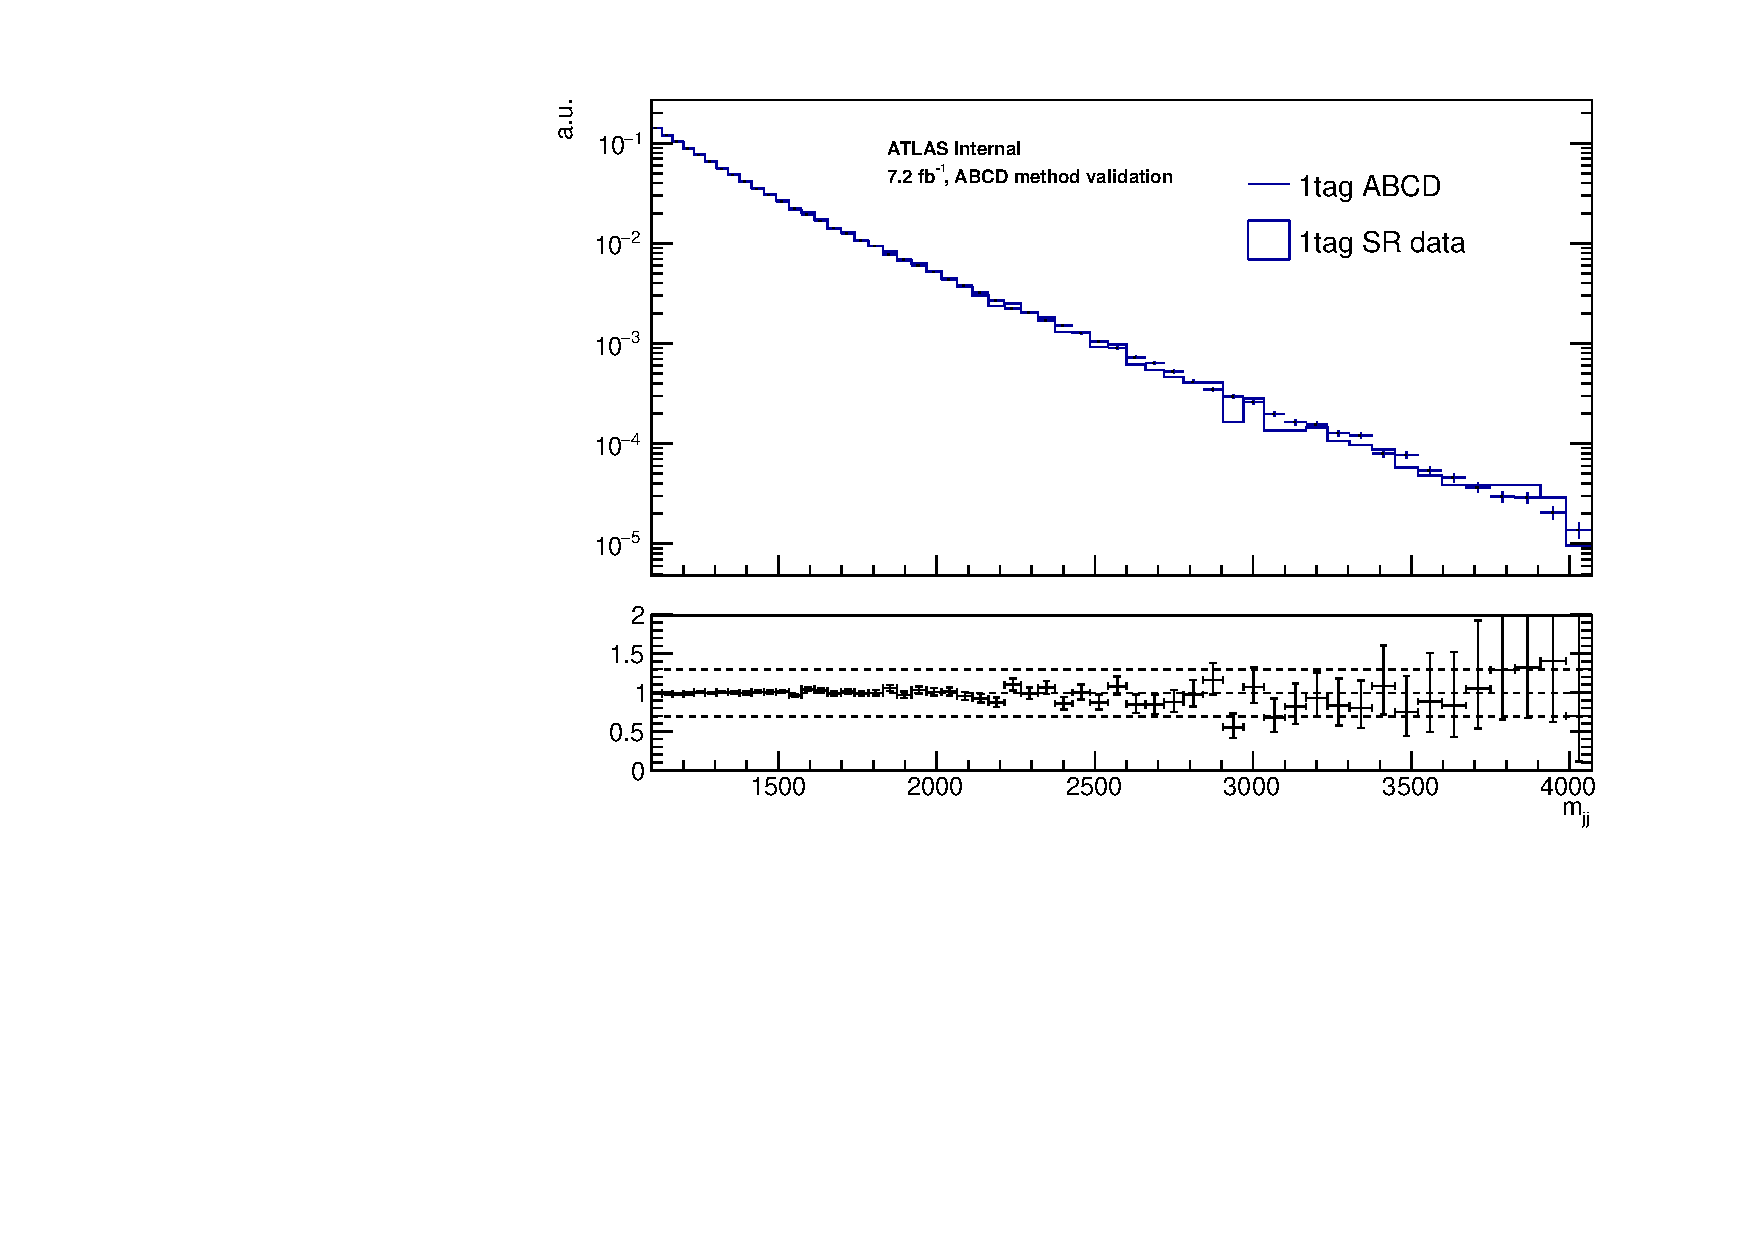
\includegraphics[width=0.45\textwidth]{figuresDijet/04-BackgroundEstimation/1tag_validationABCD.pdf}
	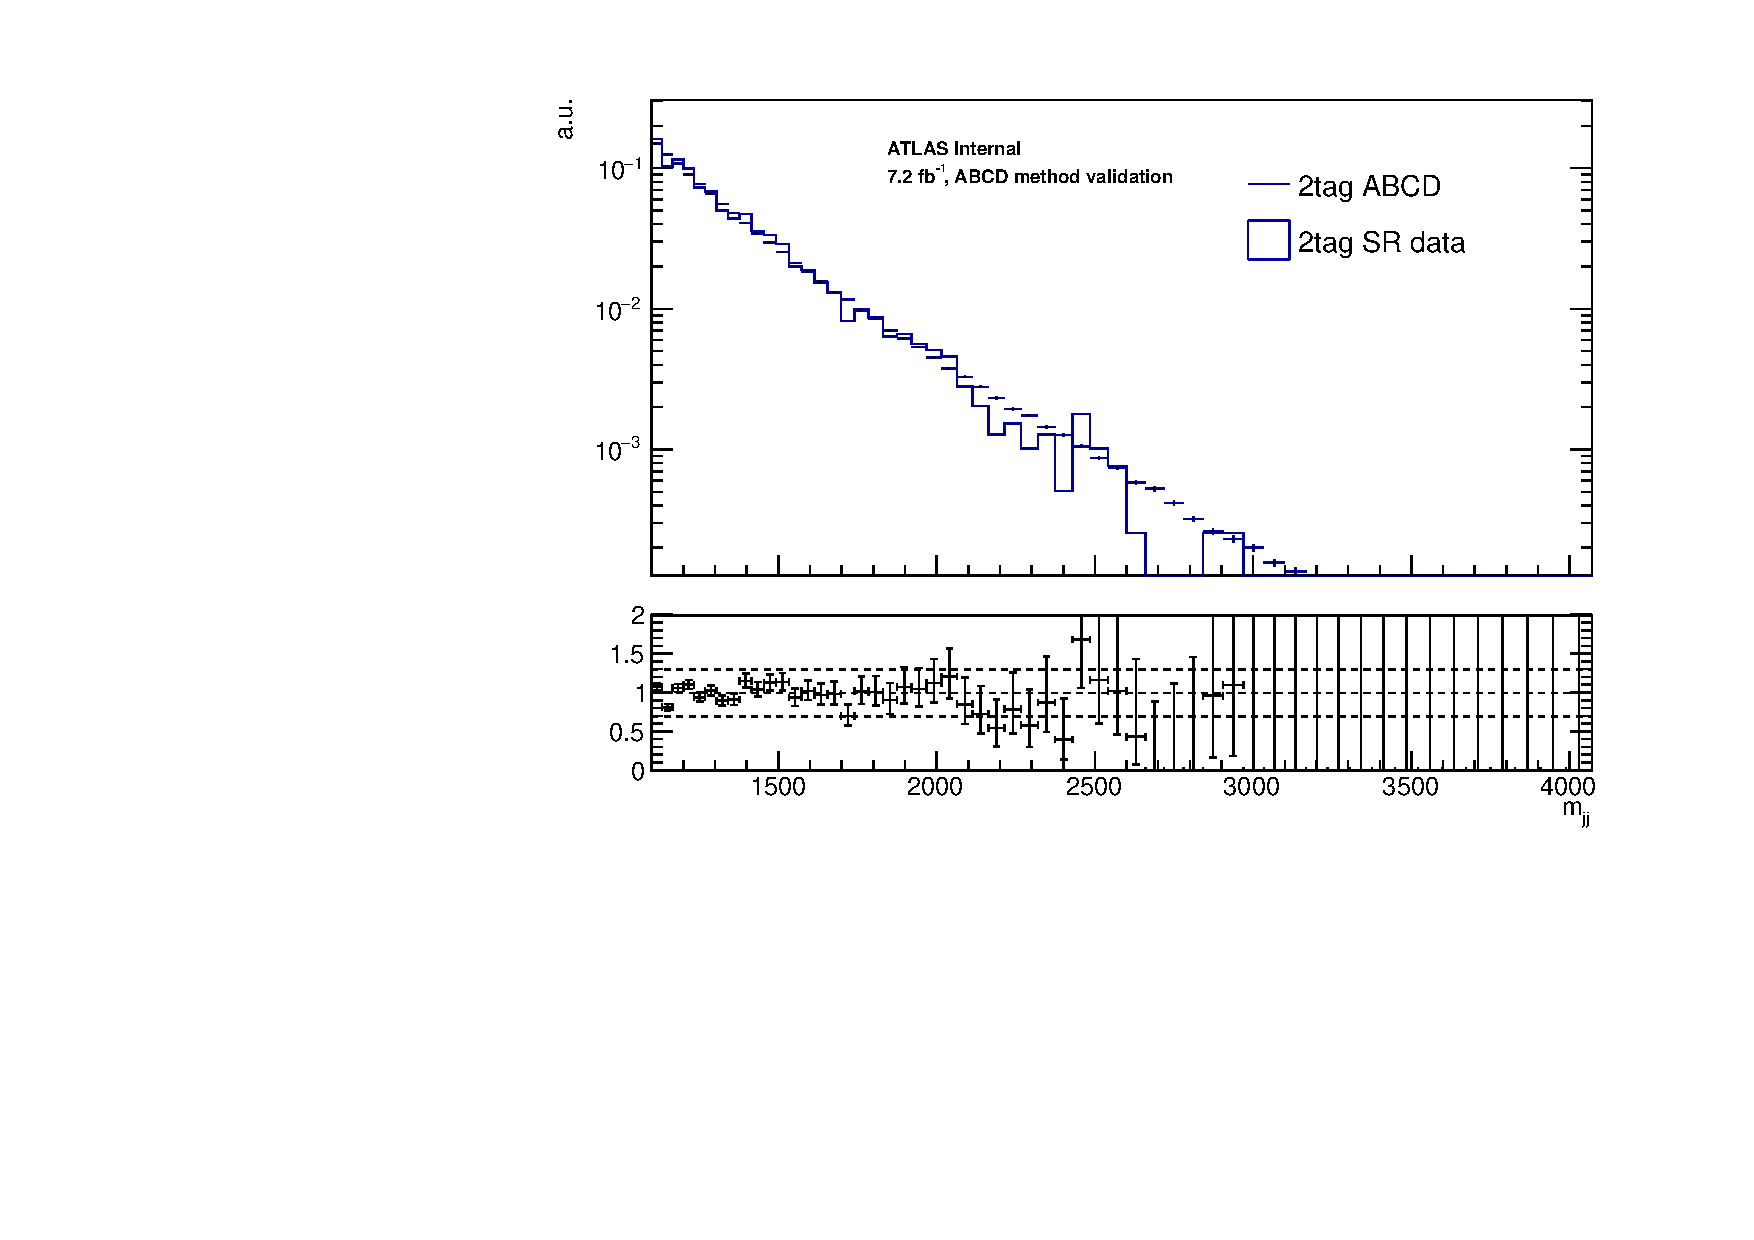
\includegraphics[width=0.45\textwidth]{figuresDijet/04-BackgroundEstimation/2tag_validationABCD.pdf}
	\caption{ABCD方法的有效性验证。左图是对于1b信号区,右图是对于2b信号区。}
	\label{fig:validationABCD}
\end{figure}


随后,我们在全部的数据上使用ABCD方法得到在1b和2b信号区$m_{jj}$本底,
并用于验证前述拟合本底策略的有效性,
如图~\ref{fig:ABCDmbb}~所示是验证结果,其中全局的$\chi^2$~p-value远大于0.05,
图中蓝色的垂线指出了被\textsc{BumpHunter}算法所标记的和拟合的本底最不一致的区间,即最突出的局部小段,
最不一致区间的统计显著性即\textsc{BumpHunter}算法p-value分别显示在图中为0.49和0.91,
这表明我们的拟合本底策略在1b和2b信号区是有效的。
图中最下面一小部分显示的是利用z-value表征的每个bin上数据与本底之前差异的显著性。

\begin{figure}[!ht]
	\centering
	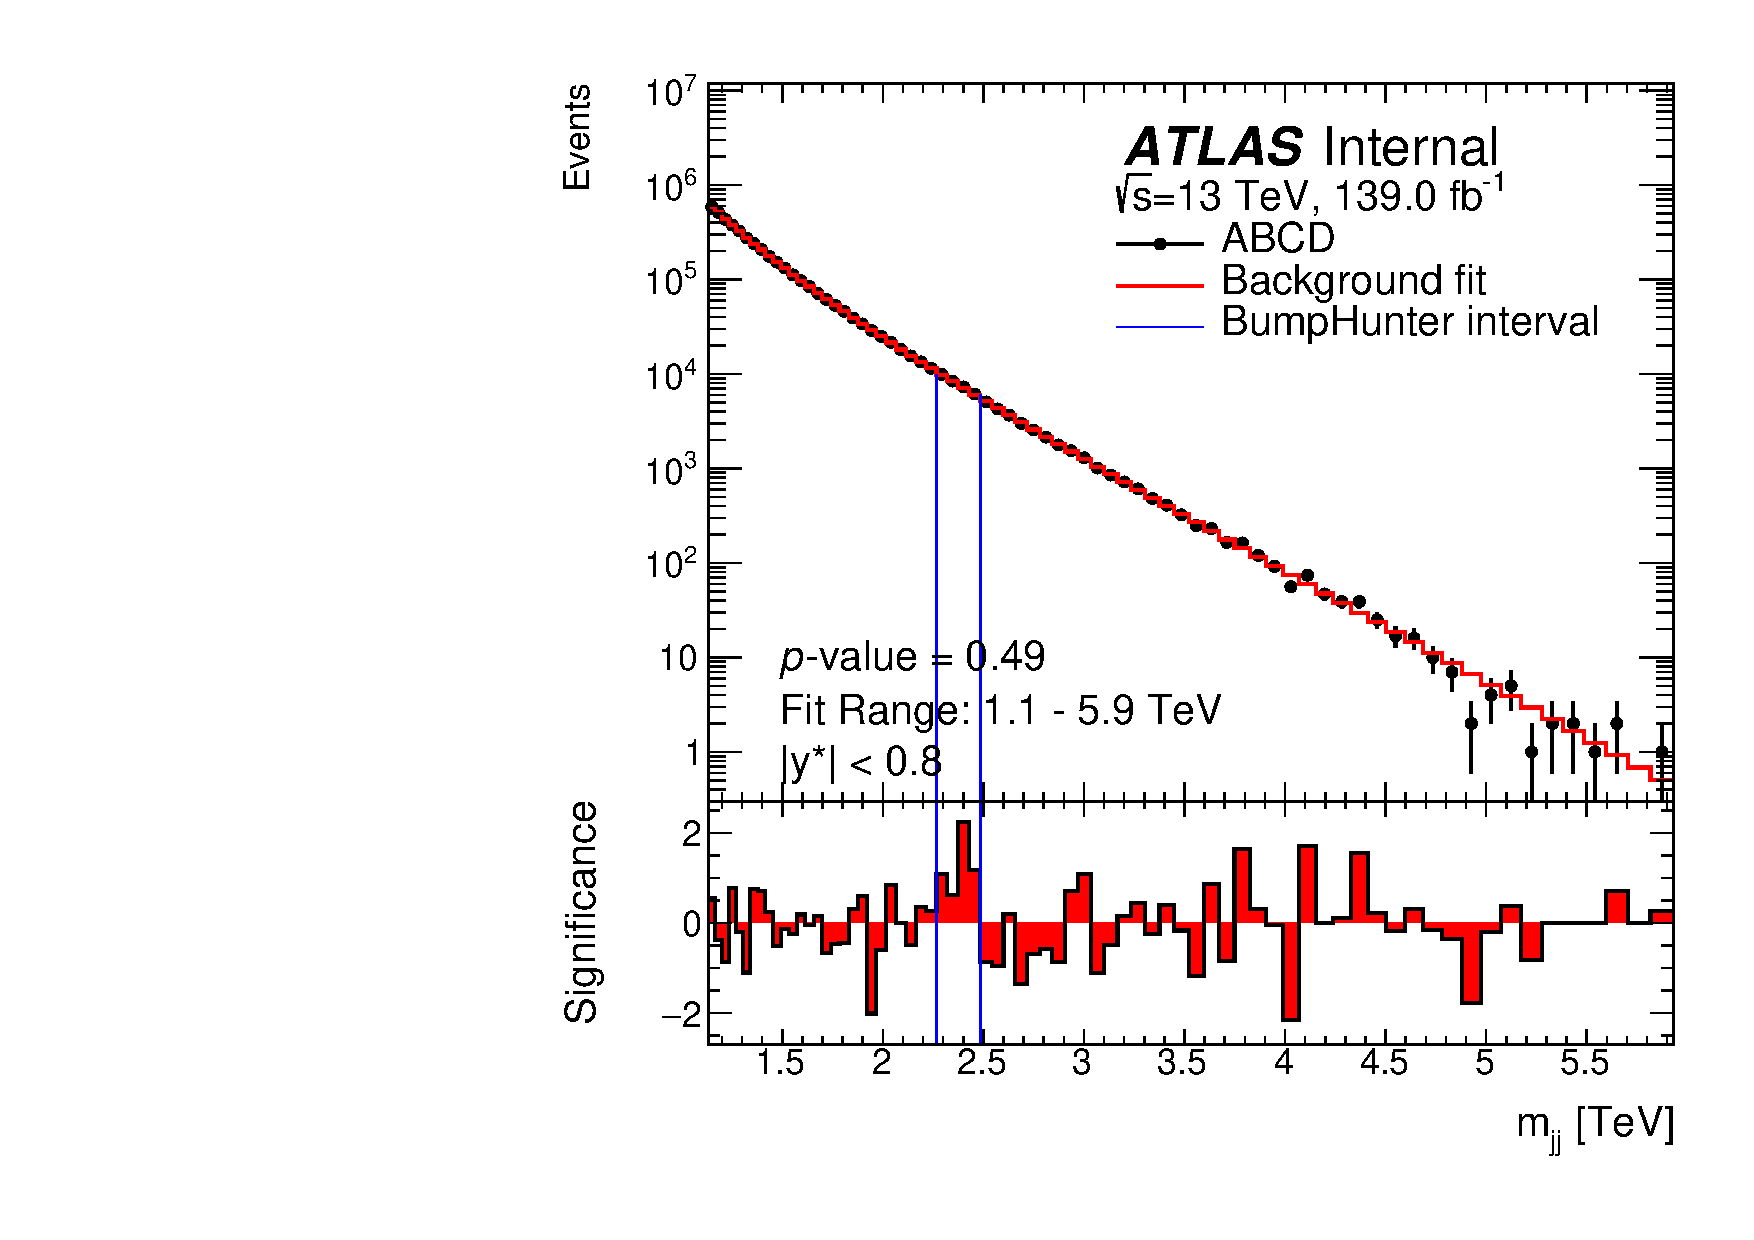
\includegraphics[width=0.45\textwidth]{figuresDijet/04-BackgroundEstimation/figure1_mbj.pdf}
	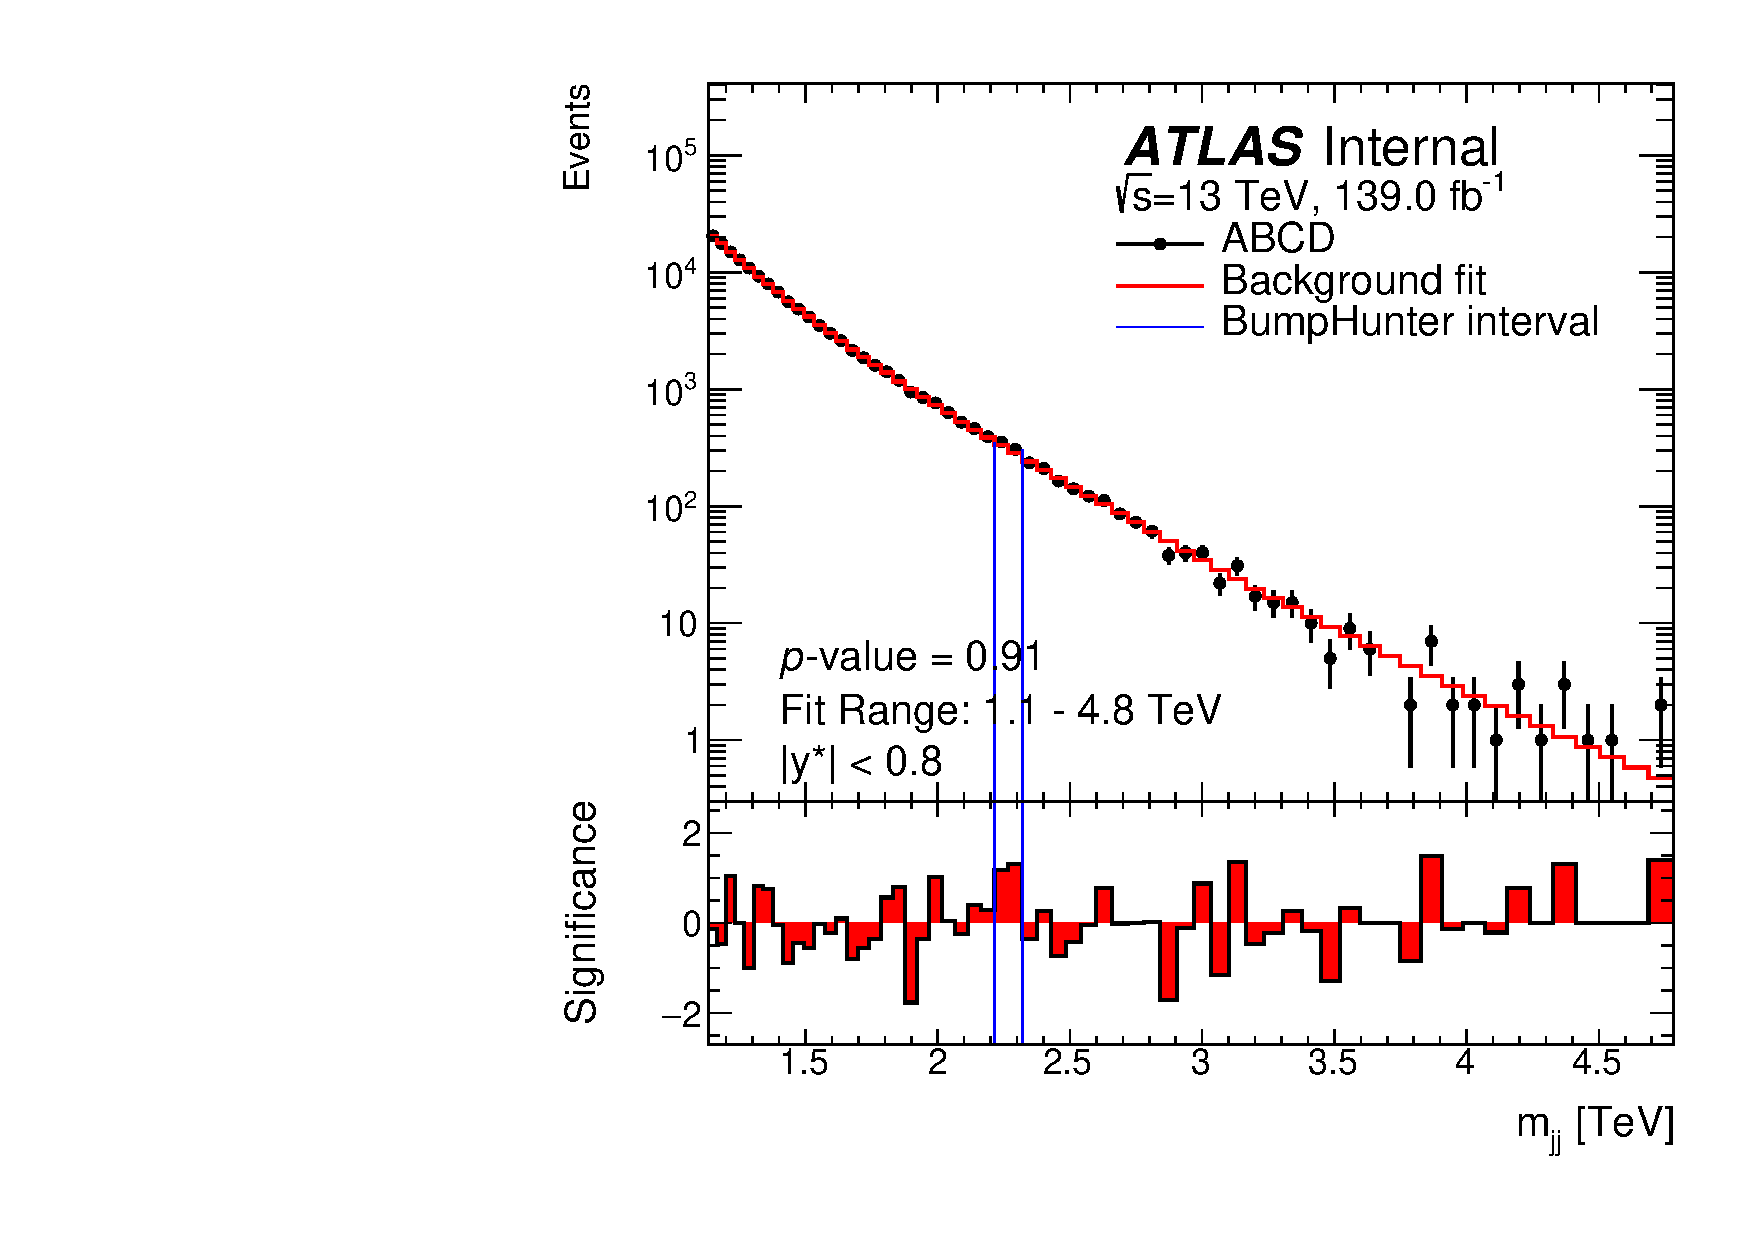
\includegraphics[width=0.45\textwidth]{figuresDijet/04-BackgroundEstimation/figure1_mbb.pdf}
	\caption{拟合本底策略的有效性验证。左图是对于1b信号区,右图是对于2b信号区,相对于拟合本底没有观察到显著的偏差。}
	\label{fig:ABCDmbb}
\end{figure}



在全包含信号区,由于没有一个合适的由本底主导的控制区,并且在使用了37$fb^{-1}$数据的类似分析当中,我们并没有发现显著的新物理信号~\cite{EXOT-2016-21},
于是我们将其中$37fb^{-1}$数据中$m_{jj}$的本底按比例放大到$139fb^{-1}$,然后对每个bin进行泊松涨落,
得到一个用于有效性验证的$m_{jj}$本底,
如图~\ref{fig:BH_stdPlot}~所示是验证结果,其中\textsc{BumpHunter}算法p-value是0.94,因此表明我们的拟合本底策略在全包含信号区也是有效的。

\begin{figure}[!ht]
        \centering
                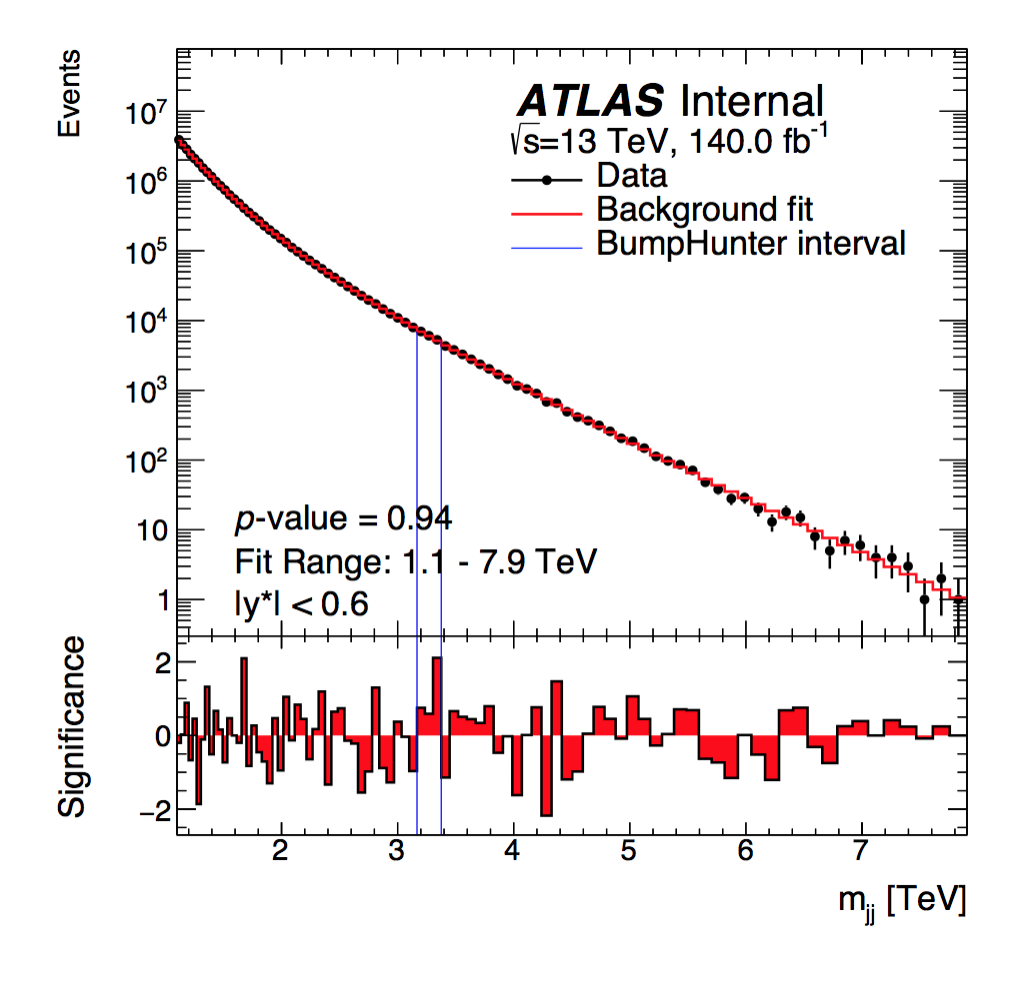
\includegraphics[width=0.75\textwidth]{figuresDijet/Appendix-BH/plain.png}
        \caption{全包含信号区中拟合本底策略的有效性验证。相对于拟合本底没有观察到显著的偏差。}
        \label{fig:BH_stdPlot}
\end{figure}


而且在这些$m_{jj}$本底上,我们还进行了信号注入测试和假信号测试来验证拟合方法的有效性。
在信号注入测试中,我们将各种模型的信号和预期的本底分布叠加,
首先我们用这种拟合本底策略和\textsc{BumpHunter}算法来测试其对新物理信号的灵敏度,
结果表明它们能成功并精准的发现信号。
接着我们会评估在信号注入的窗口中用信号加本底能否成功的拟合这些组合起来的分布并正确的测量信号产出,
我们发现,对于每个基准信号和标准的高斯信号,在统计误差范围内,这种拟合本底方法所提取出来的信号量与注入信号量一致。
在假信号测试中,对于不同的信号模型和信号质量,我们用信号加本底拟合$m_{jj}$本底,所拟合出来的信号量作为假信号的评估标准,
这些测试是为了评估拟合本底策略的稳健性和拟合函数对信号的建模能力。
在全包含信号区,除了相对宽度\footnote{相对宽度定义为$\frac{\sigma_x}{m_x}$,$\sigma_x$其中是信号宽度,$m_x$为信号质量。}
为$15\%$的高斯信号,其他信号的假信号测试都没有表现出显著的偏差。
对于相对宽度为$15\%$的高斯信号,在数据量很小的高质量区间,拟合出来的假信号量高达被评估的本底的统计误差的$12\%$。
在1b和2b信号区,对于所有的信号,拟合出来的假信号量都在被评估的本底的统计误差的$10\%$到$20\%$之间。
如第~\ref{sec:DijetSys}~节所述,我们为每个受影响的信号引入了一个相应的系统误差。


\subsection{搜索结果}
\label{sec:DijetMjj4}


图~\ref{fig:dijetspectra}~展示的是实际的数据中三个不同信号区所观测到的$m_{jj}$分布及相应的拟合和搜索结果。
每个信号区中不同质量点的bin宽都近似等于所对应质量点$m_{jj}$的分辨率,它会随着$m_{jj}$质量的增大而变大。
为了在图中直观显示搜索的信号,我们将所预测的基准信号放大了10倍到1000倍不等。
图中蓝色的垂线指出了被\textsc{BumpHunter}算法所标记的和本底最不一致的区间即最突出的局部小段。
在全包含信号区,对于$|y^*|<0.6$和$|y^*|<1.2$的筛选条件,全局的$\chi^2$~p-value分别为0.08和0.078,
最不一致区间的统计显著性即\textsc{BumpHunter}算法p-value分别为0.89和0.88。
在1b和2b信号区,全局的$\chi^2$~p-value分别是0.92和0.16,
最不一致区间的\textsc{BumpHunter}算法p-value分别为0.69和0.83,
因此在全本底的假设下,我们在来自数据的$m_{jj}$谱上没有观察到明显的偏离。
图~\ref{fig:dijetspectra}~中最底部的一小部分展示的是利用z-value表征的每个bin中数据和本底之间差异的显著性,
这部分使用的是泊松分布且仅仅考虑了统计误差。




\begin{figure}[htbp]
  \begin{subfigure}{.5\textwidth}
  \centering
  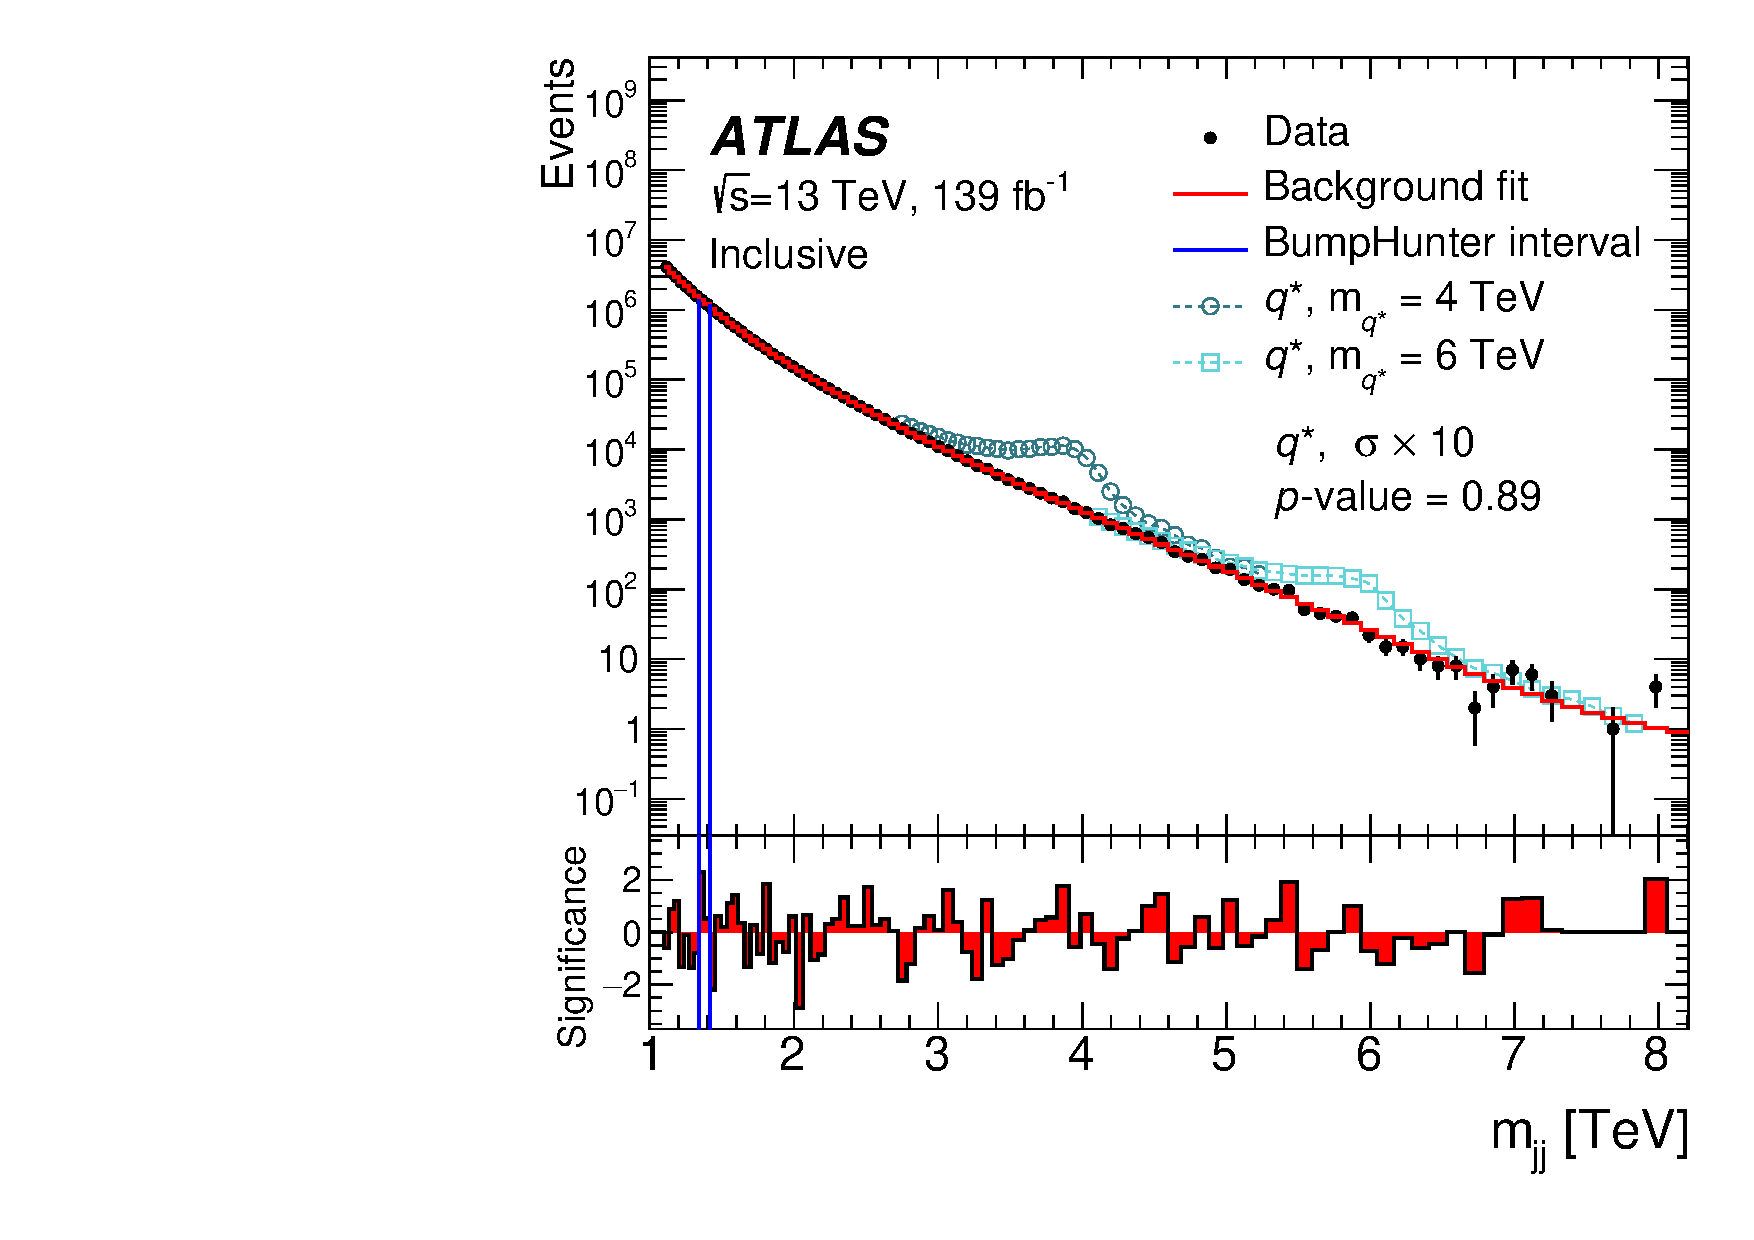
\includegraphics[width=0.9\textwidth]{figs/fig_03a.pdf}
  \caption{}
  \end{subfigure}
  \begin{subfigure}{.5\textwidth}
  \centering
  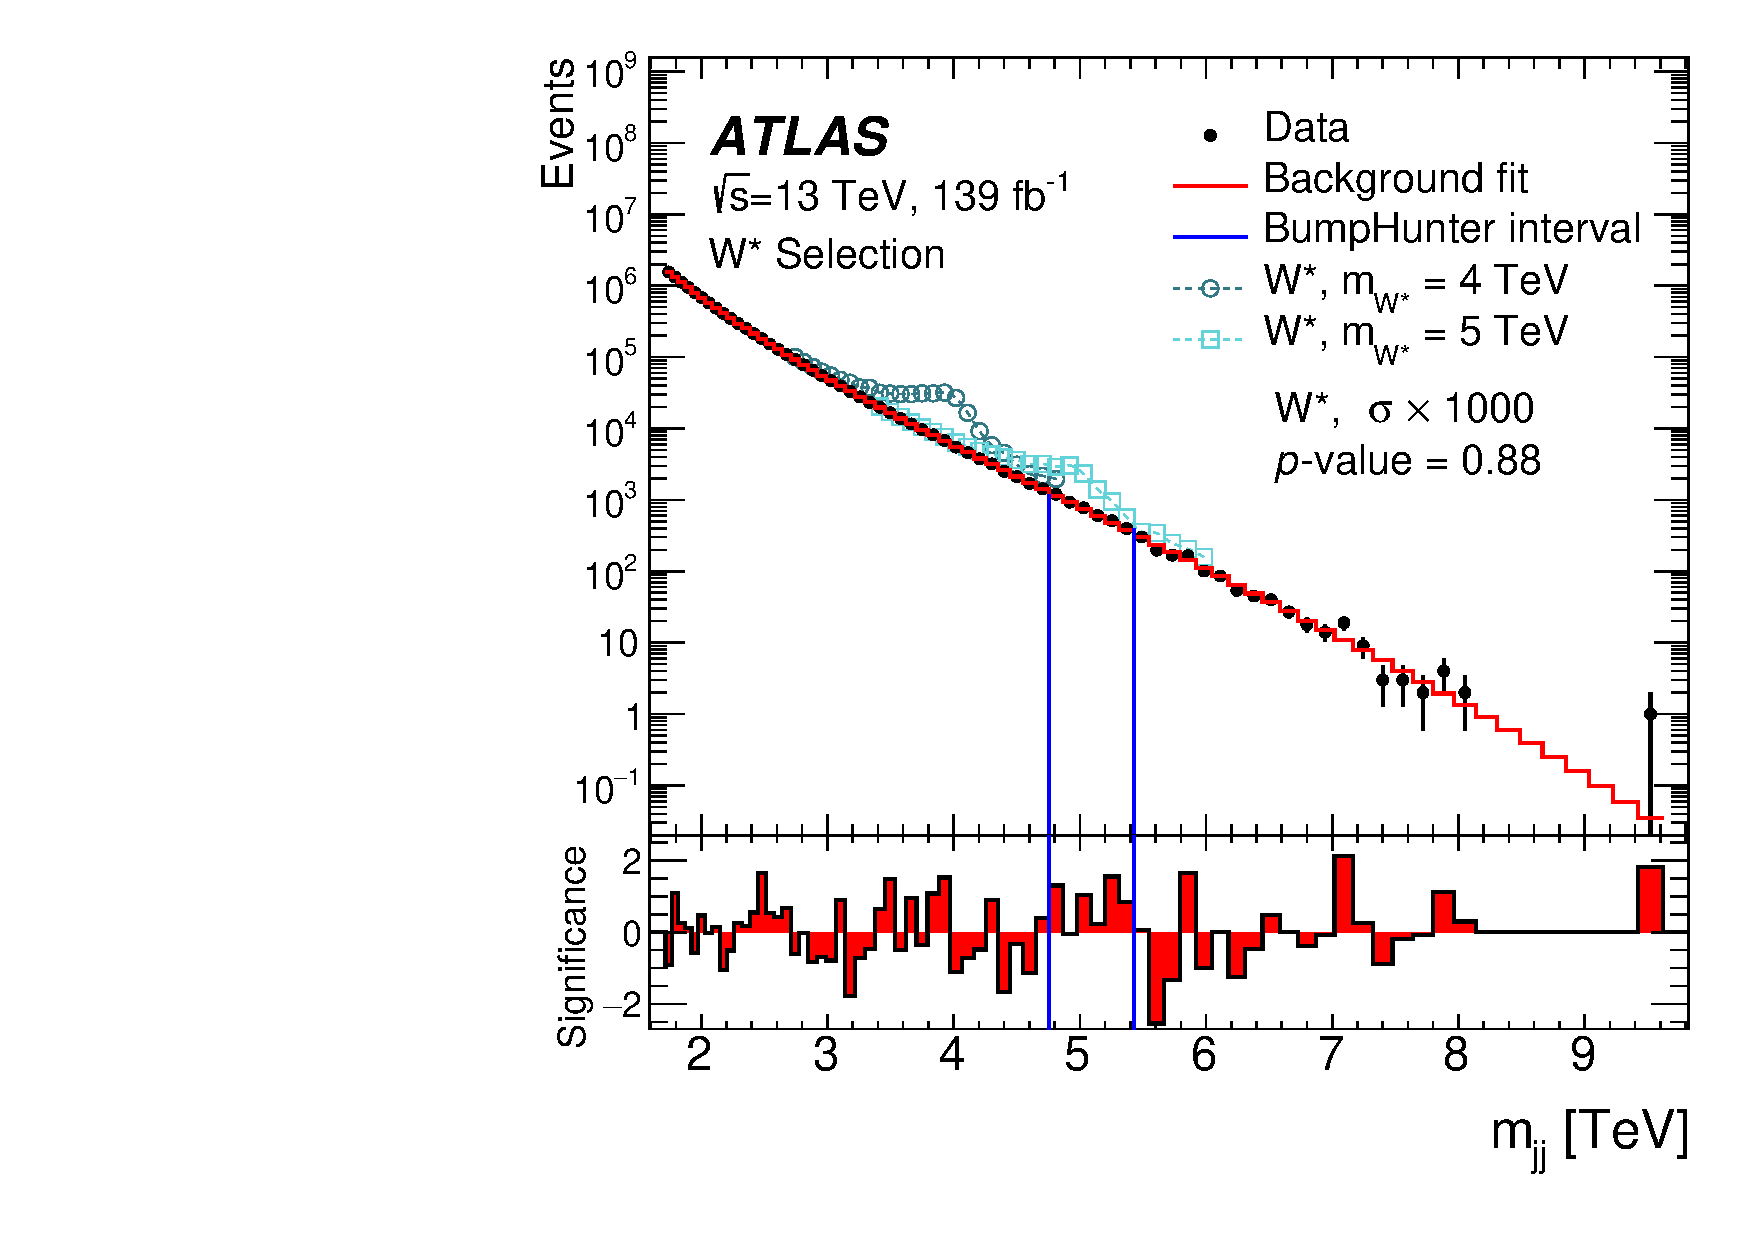
\includegraphics[width=0.9\textwidth]{figs/fig_03b.pdf}
  \caption{}
  \end{subfigure}
\newline
  \begin{subfigure}{.5\textwidth}
  \centering
  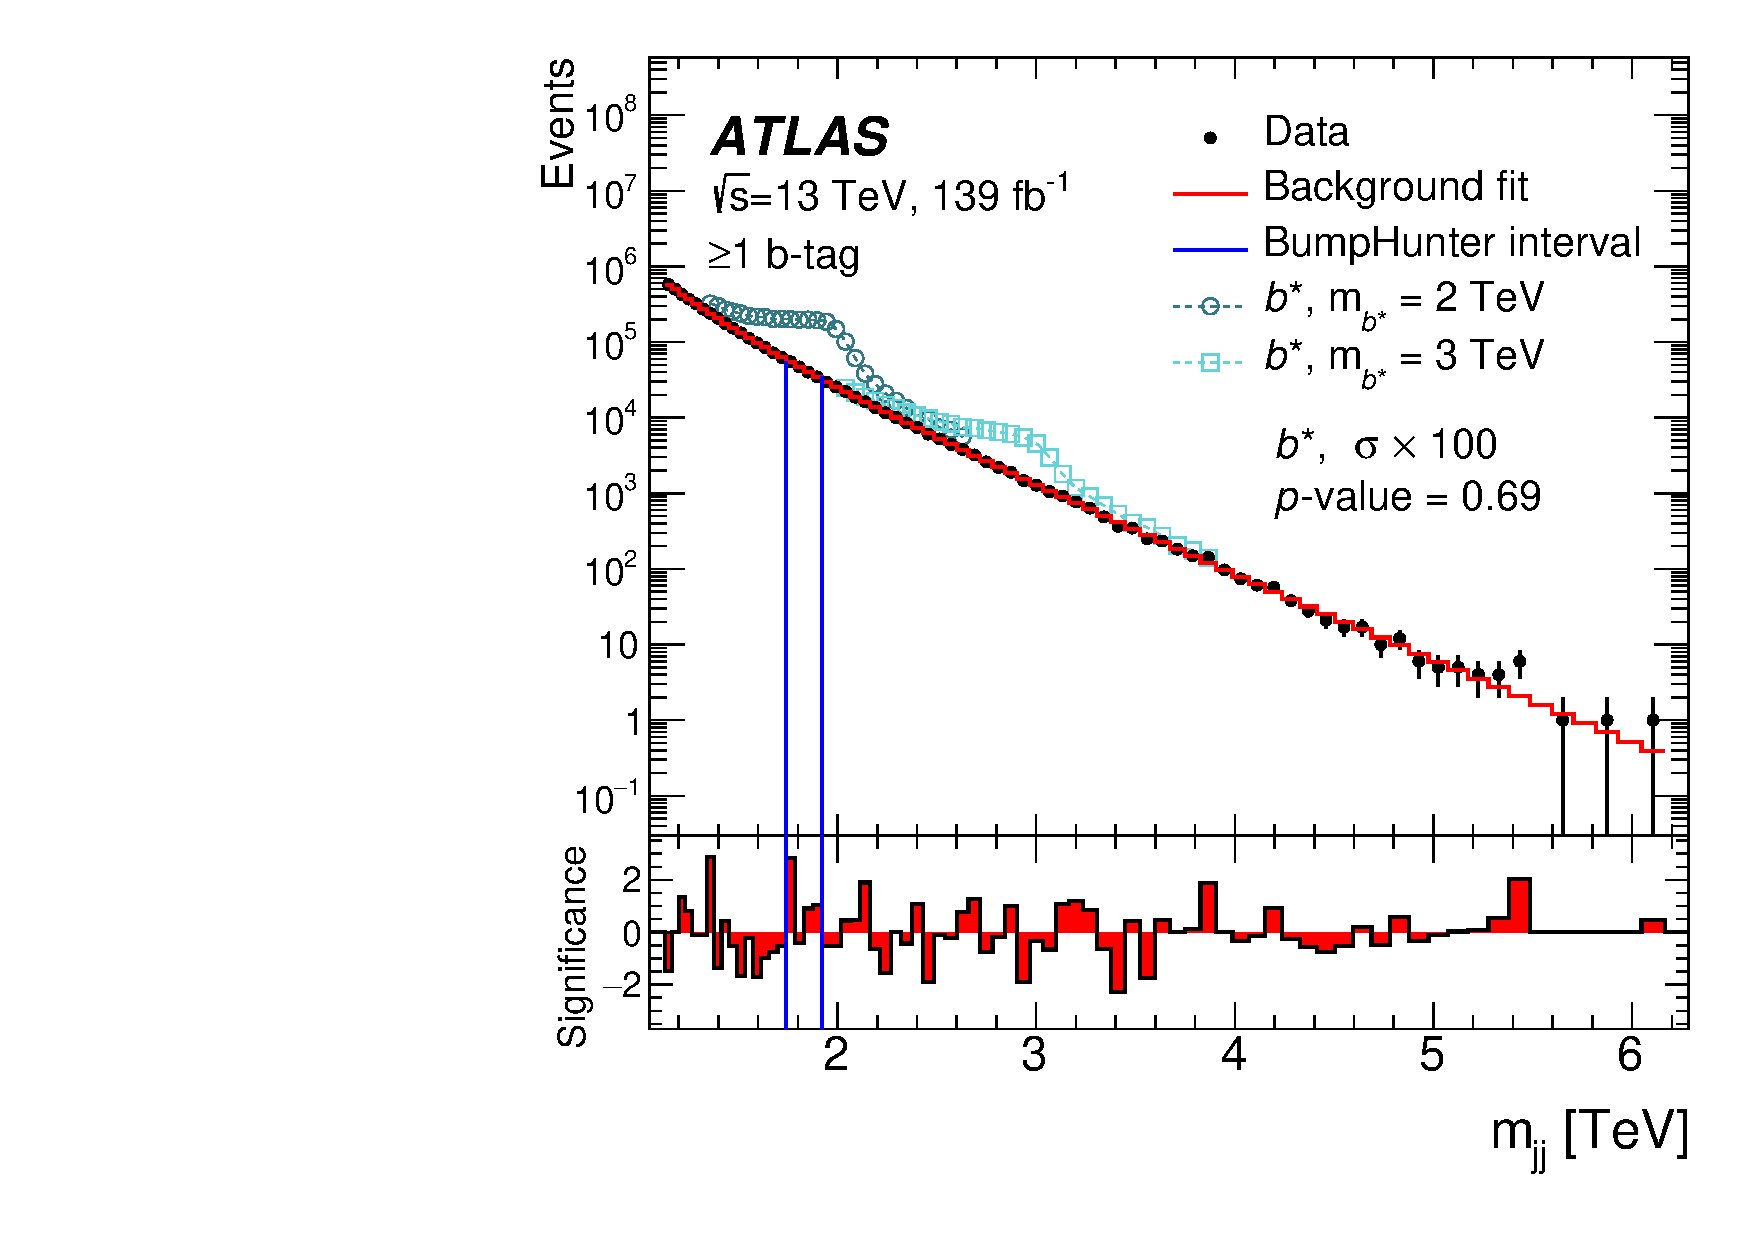
\includegraphics[width=0.9\textwidth]{figs/fig_03c.pdf}
  \caption{}
  \end{subfigure}
  \begin{subfigure}{.5\textwidth}
  \centering
  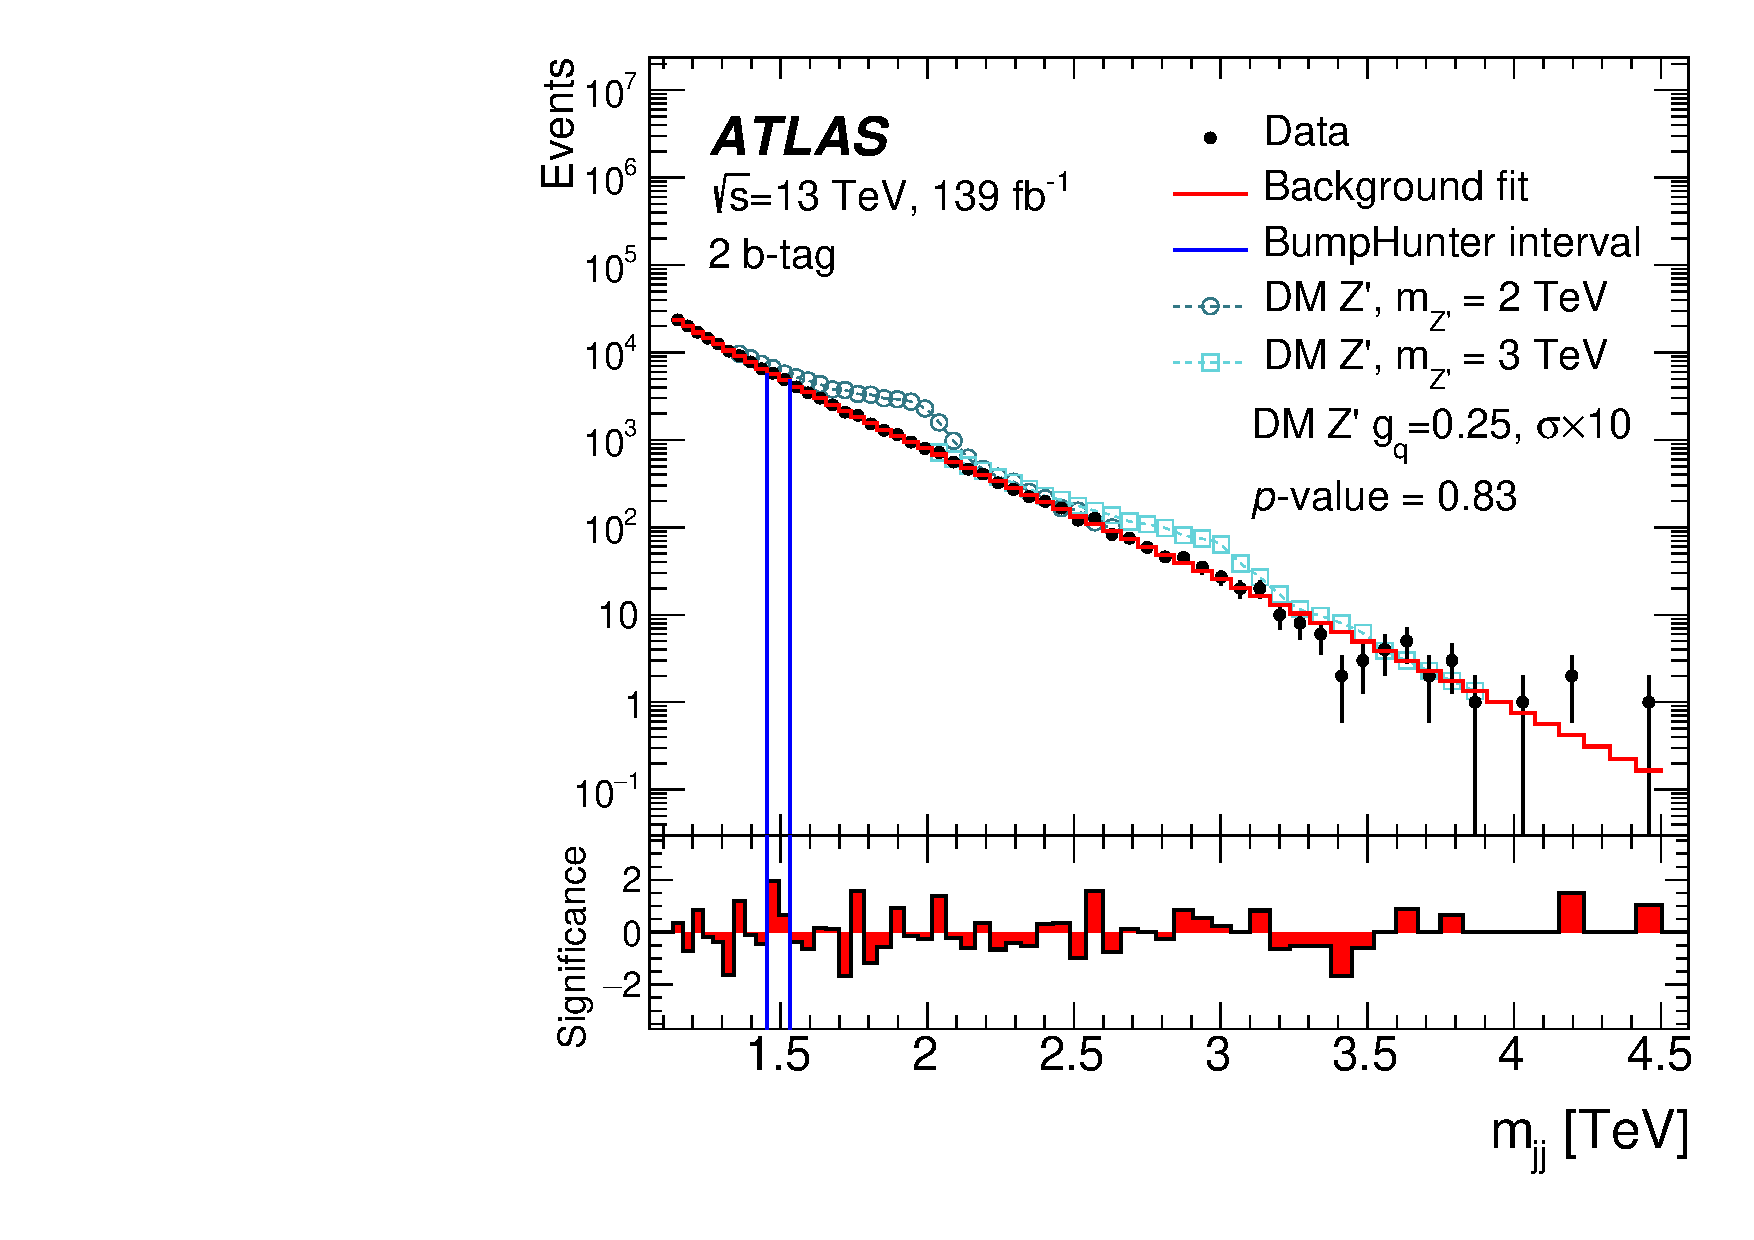
\includegraphics[width=0.9\textwidth]{figs/fig_03d.pdf}
  \caption{}
  \end{subfigure}
  \caption{
 不同信号区所观测到的不变质量谱$m_{jj}$的分布:(a) 全包含信号区,$|y^*|<0.6$的筛选条件;(b) 全包含信号区,$|y^*|<1.2$的筛选条件;(c) 1b信号区;(d) 2b信号区。
 蓝色的垂线指出了被\textsc{BumpHunter}算法所标记的和拟合的本底最不一致的区间,且对应的\textsc{BumpHunter}算法p-value也有在图中显示。  }
  \label{fig:dijetspectra}
\end{figure} 



\section{系统误差} 
\label{sec:DijetSys}


\subsection{本底误差} 
\label{sec:DijetSysBkg}

我们考虑了两种影响本底估计的系统误差,它们分别是由数据样本大小限制所带来的拟合误差和由拟合函数的选择所带来的选择误差。
为了估计这些误差,我们使用标准的$m_{jj}$本底通过泊松涨落产生了大量($\sim 10\,000$)的赝数据(pseudo-data),
本节中提到的所有误差都是指相对于标准值(nominal values)的变化。
拟合误差是通过在那些赝数据上重复第~\ref{sec:DijetMjj}~节中本底拟合过程得到的,
$m_{jj}$中每个bin的拟合误差是所有赝数据在对应的bin的拟合结果的均方根,
除了对于全包含信号区$|y^*|<1.2$的情形,
其在$m_{jj}=2TeV$时大约为$0.1\%$,在高质量的尾部区域增加到$30\%\text{--}40\%$,
对于全包含信号区$|y^*|<1.2$的情形,尾部比较长,在高质量区间$m_{jj}=9.6TeV$左右有一个孤立的事例,拟合误差较大,
但是在$m_{jj}=8TeV$左右,拟合误差也在$30\%\text{--}40\%$。



而选择误差是通过用标准函数(nominal function)和备选函数(alternative parametric functions)分别拟合那些赝数据得到的,这里和本节后文的拟合也都是指滑动窗口拟合。
标准函数指式~\ref{eq:Mjj1}~中的参数函数,
为了决定备选函数的形式,我们进行了多种尝试,每次拟合的函数相对于标准函数最多具有一个附加的自由参数,
在要求其满足拟合质量标准的同时,拟合结果与标准函数的拟合结果差异最大的那个函数将作为用来评估选择误差的备选函数。
在全包含信号区,所决定的备选函数形式是$f(x)=p_1(1-x)^{p_2}x^{p_3+p_4\ln x+p_5x}$,在1b和2b信号区,所决定的备选函数都为$f(x)=p_1(1-x)^{p_2+p_3 x}x^{p_4 +p_5\ln x}$,
有了标准函数和备选函数之后,我们将用两种函数分别拟合的结果之间差异的平均值作为选择误差其在高质量区域达到了$10\%$。
图~\ref{fig:Syst1}~展示了三个信号区中影响本底估计的两种系统误差。


\begin{figure}[!thbp]
  \begin{subfigure}{.5\textwidth}
  \centering
  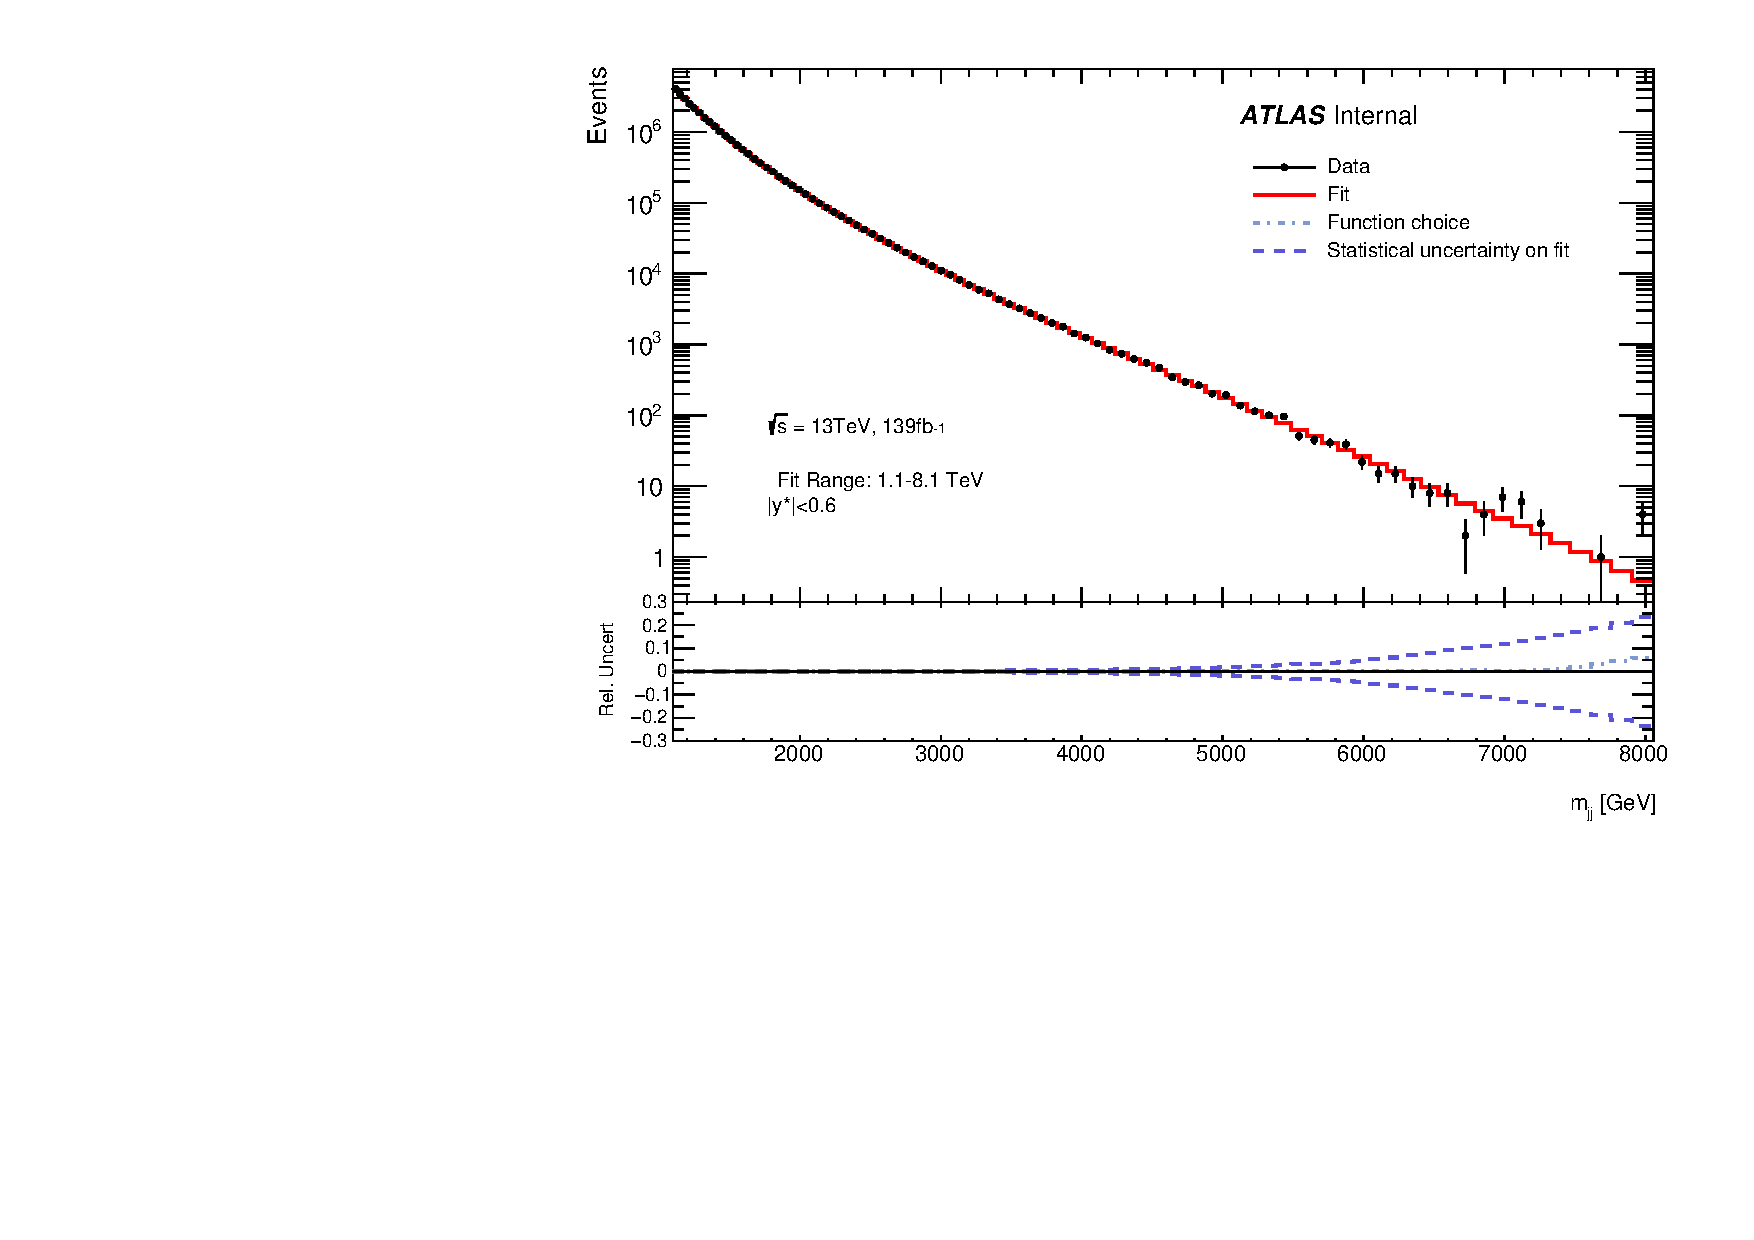
\includegraphics[width=0.9\textwidth]{figuresDijet/07-SystematicUncertainties/uncertQ1.pdf}
  \caption{}
  \end{subfigure}
  \begin{subfigure}{.5\textwidth}
  \centering
  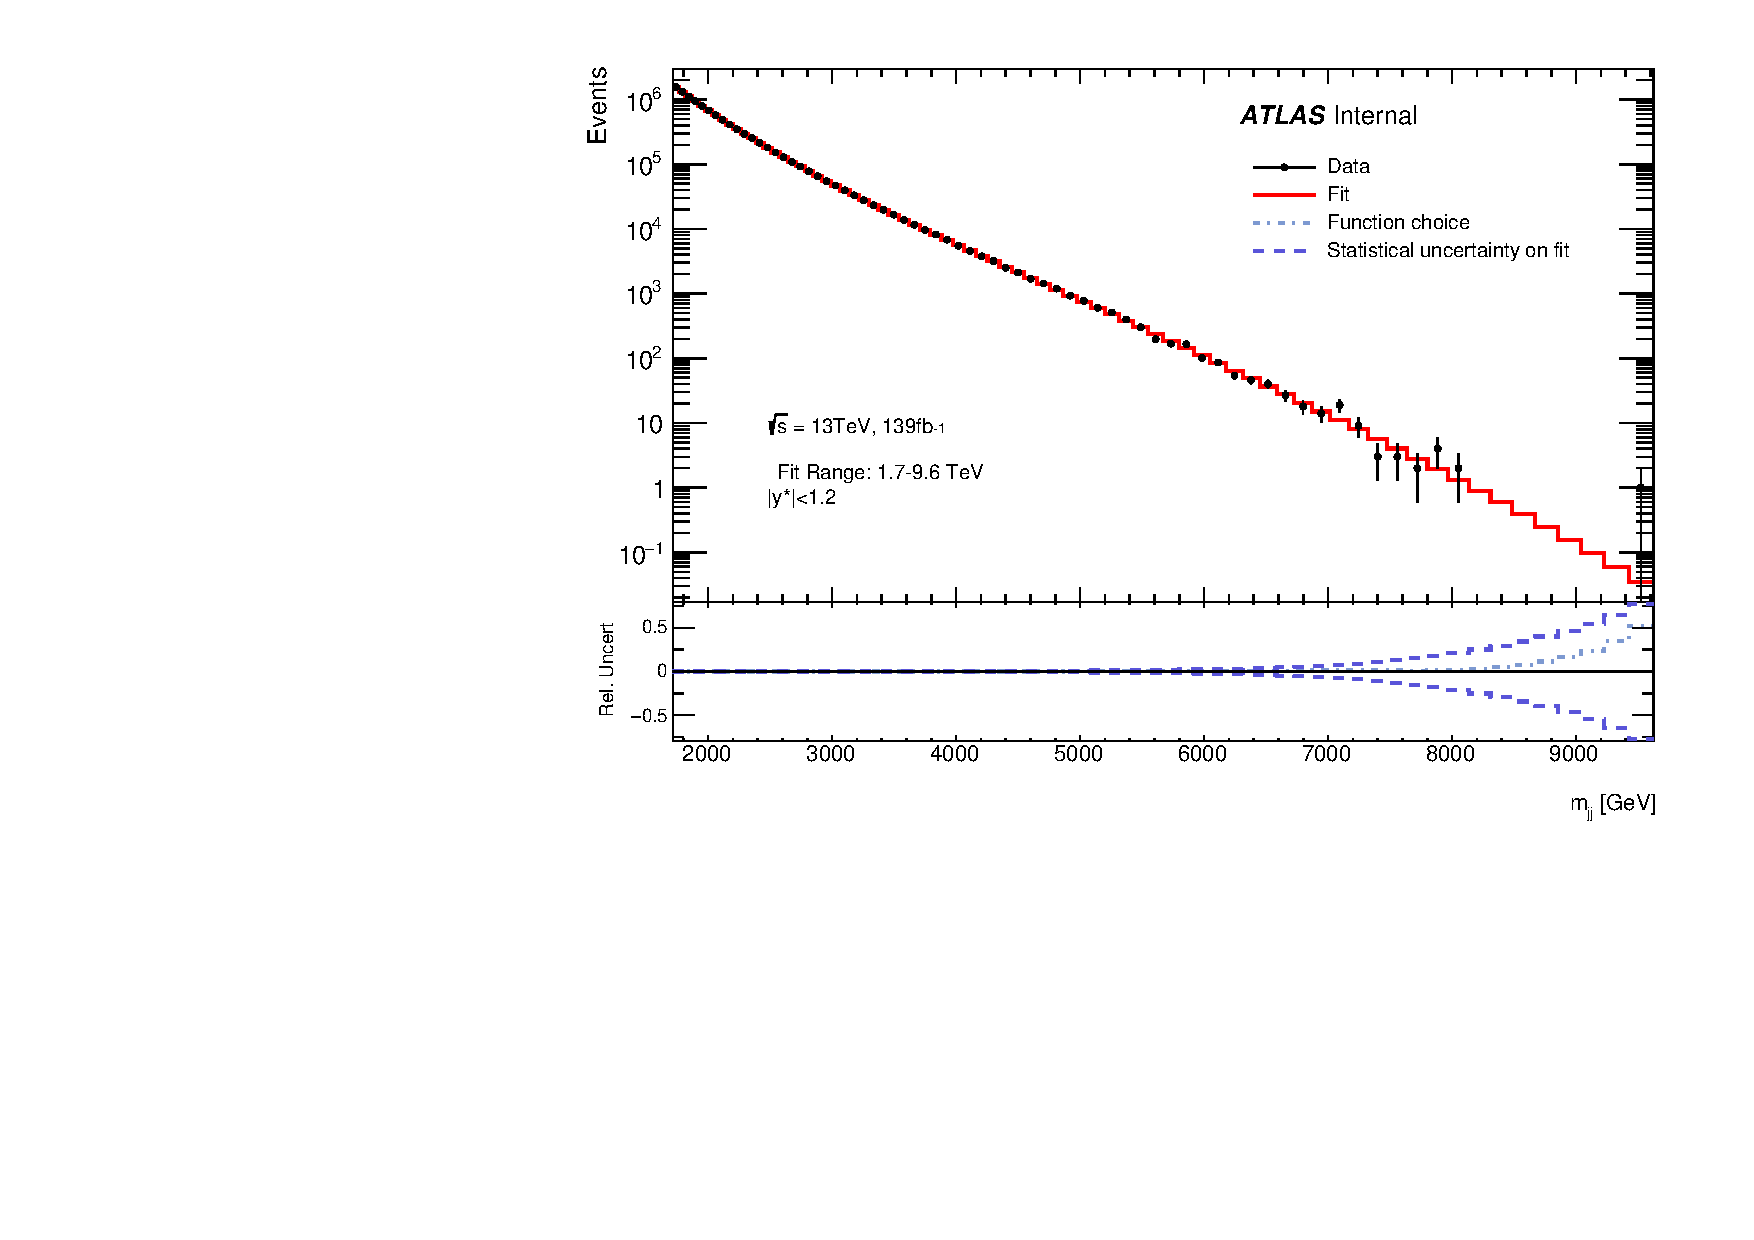
\includegraphics[width=0.9\textwidth]{figuresDijet/07-SystematicUncertainties/uncertWstar.pdf}
  \caption{}
  \end{subfigure}
\newline 
  \begin{subfigure}{.5\textwidth}
  \centering
  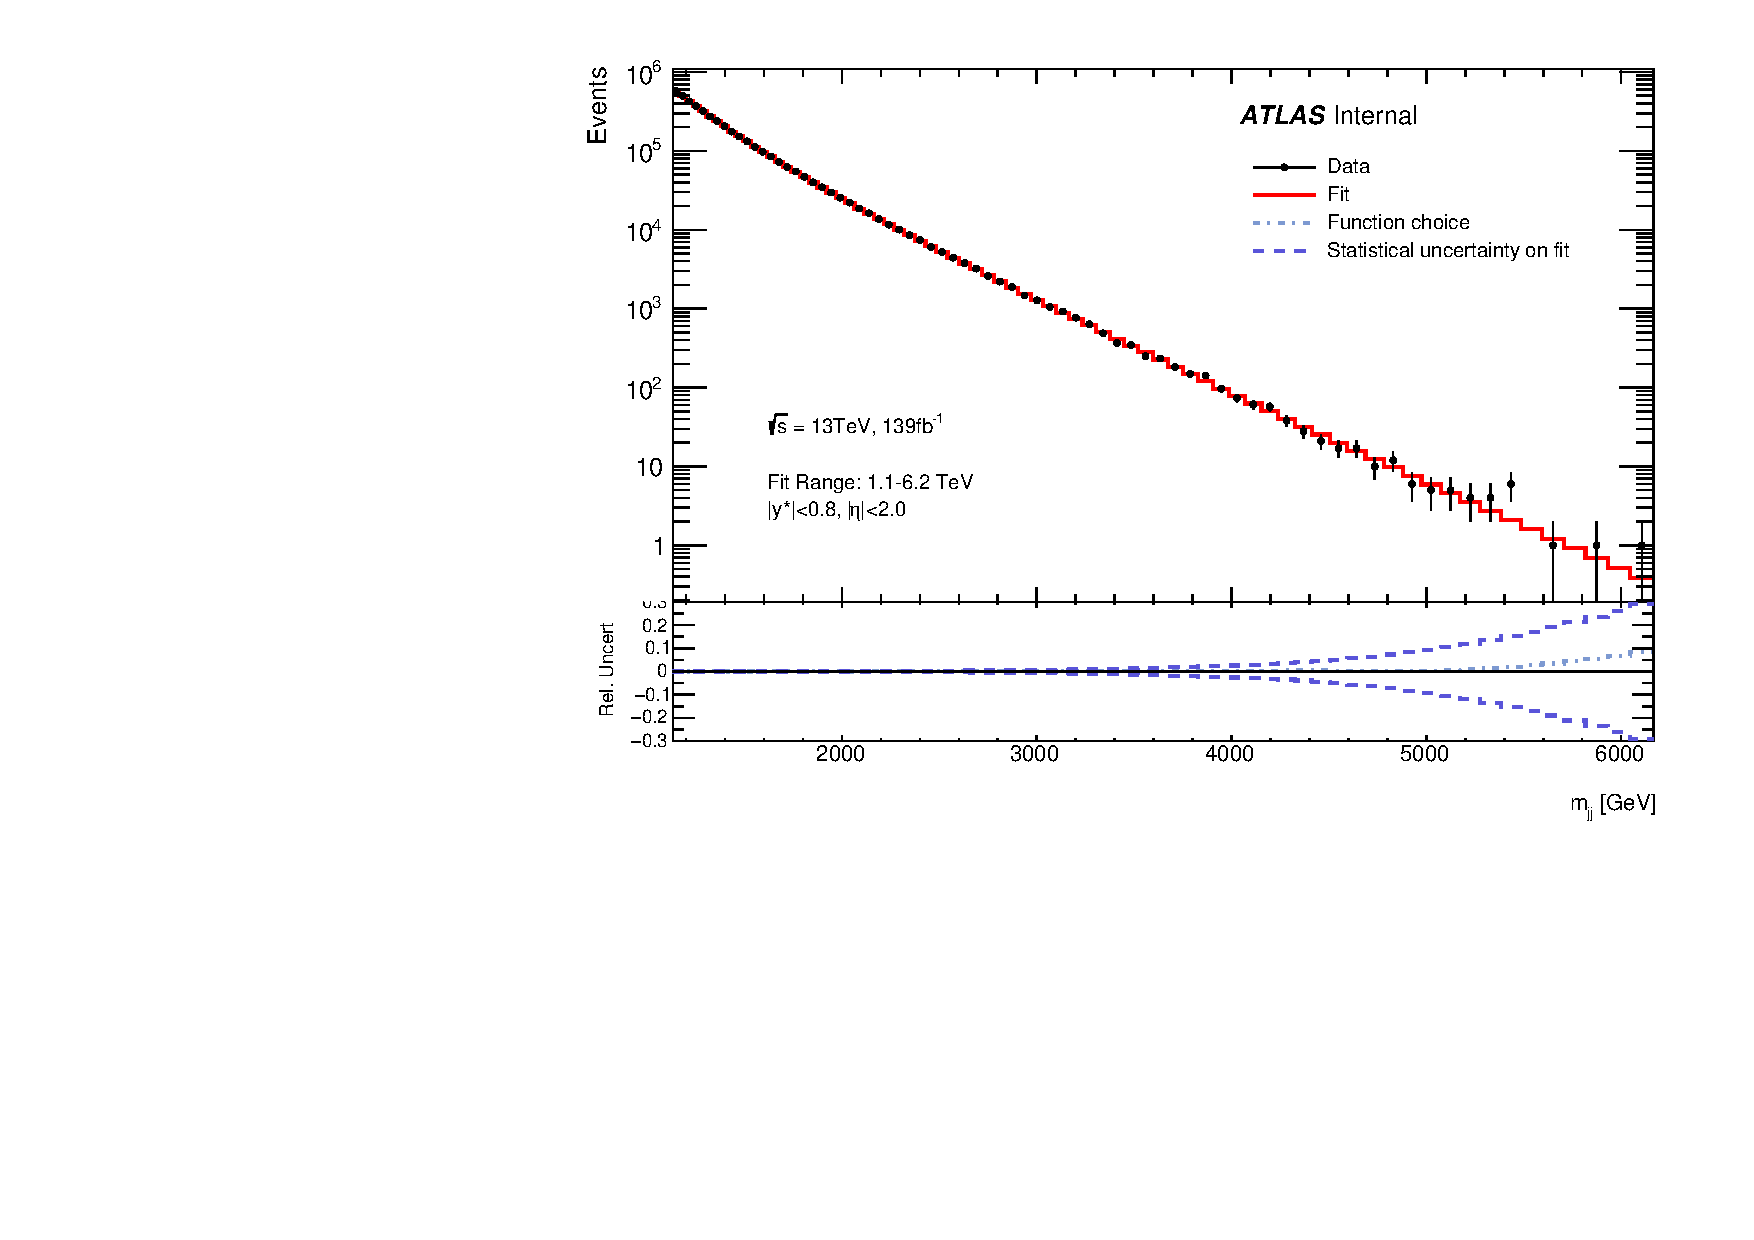
\includegraphics[width=0.9\textwidth]{figuresDijet/07-SystematicUncertainties/uncertmbj.pdf}
  \caption{}
  \end{subfigure}
  \begin{subfigure}{.5\textwidth}
  \centering
  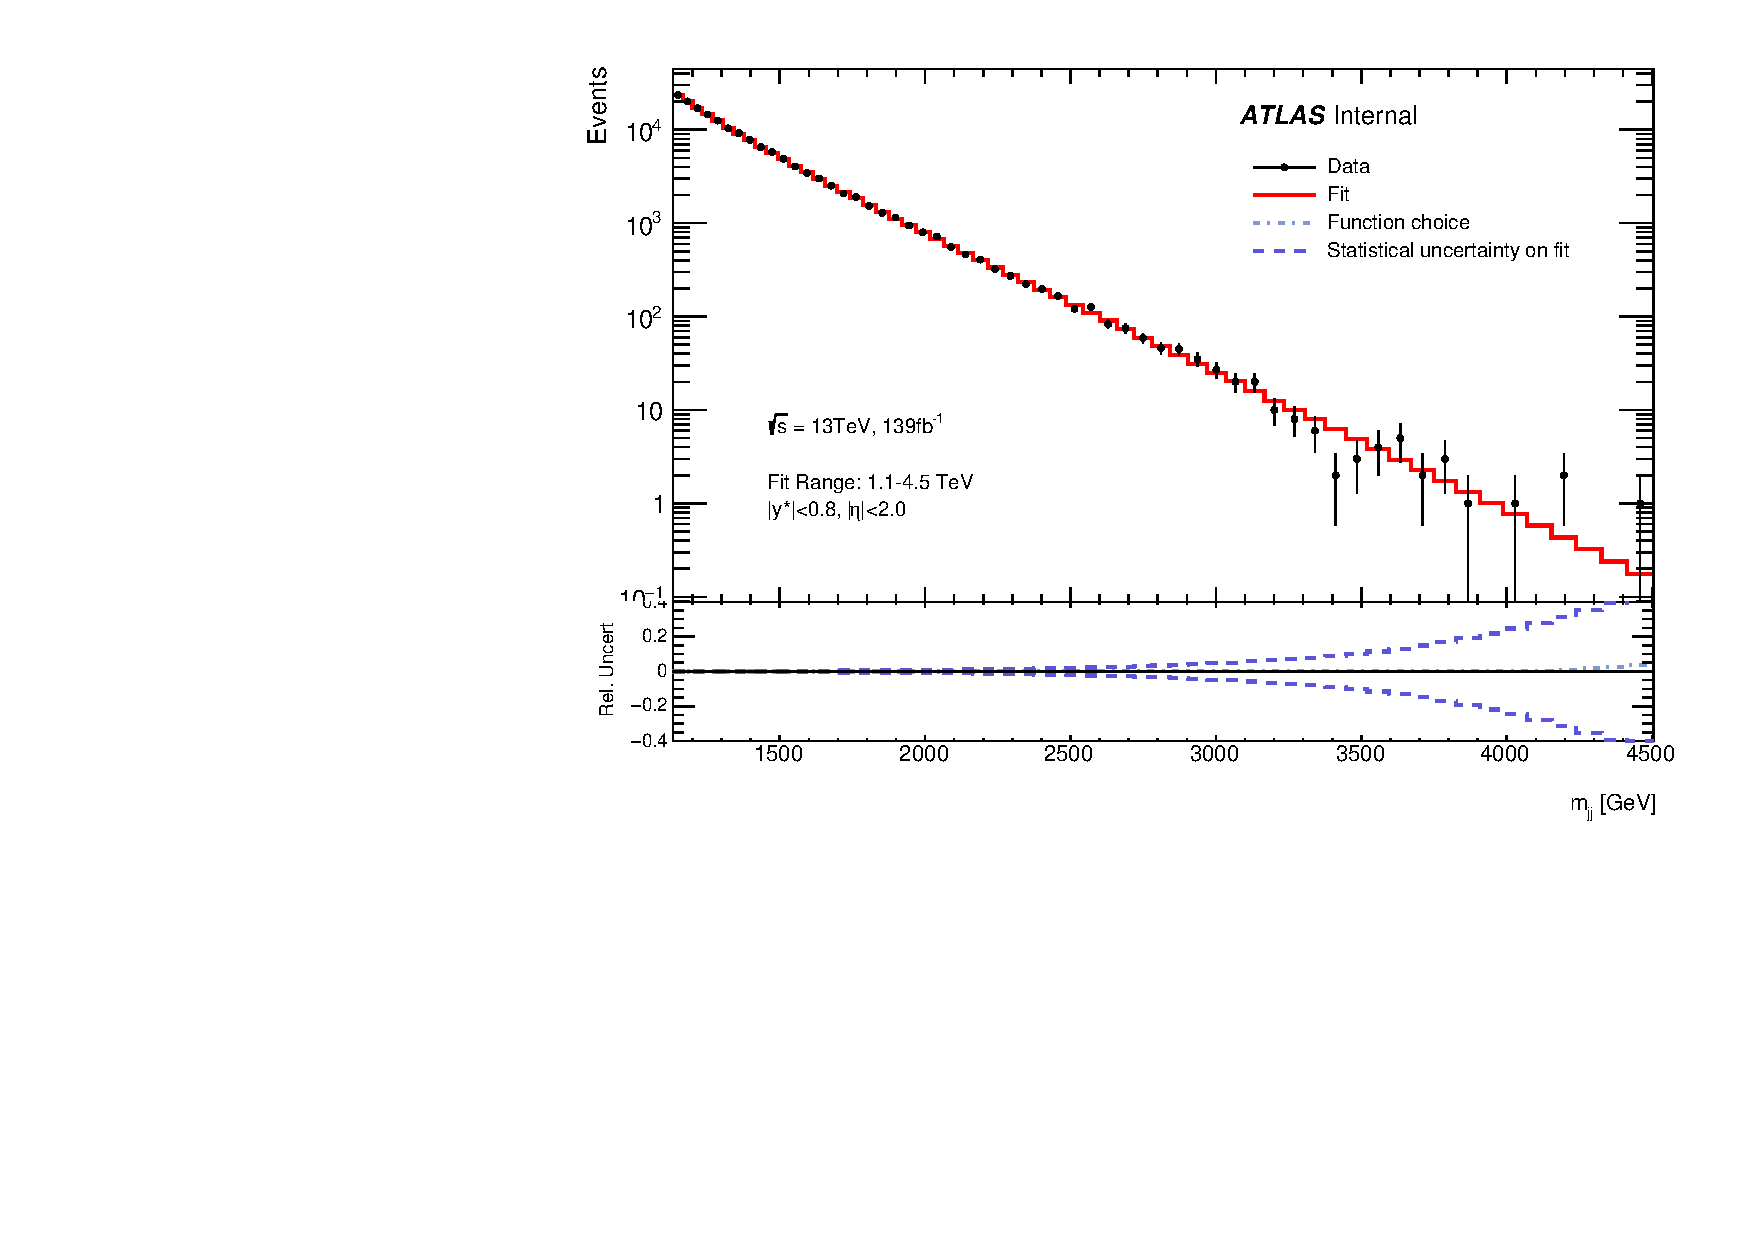
\includegraphics[width=0.9\textwidth]{figuresDijet/07-SystematicUncertainties/uncertmbb.pdf}
  \caption{}
  \end{subfigure}
  \caption{
   不同信号区中影响本底估计的两种系统误差,其中深蓝色的虚线表示拟合误差,浅蓝色虚线表示选择误差:
   (a) 全包含信号区,$|y^*|<0.6$的筛选条件;(b) 全包含信号区,$|y^*|<1.2$的筛选条件;(c) 1b信号区;(d) 2b信号区。
}
\label{fig:Syst1}
\end{figure}



另外我们还考虑了一种影响本底建模基于第~\ref{sec:DijetMjj}~节假信号测试的系统误差。 
在全包含信号区,仅对于相对宽度为$15\%$的高斯信号,这种假信号误差才被考虑进去,
因为对于其他信号,没有看到明显的偏差。
在1b和2b信号区,根据所观测到的影响大小,我们针对每个不同的信号,分别考虑了这种假信号误差。
%研究表明这种假信号误差在信号散射截面的影响要小于所有考虑到的基准信号和高斯信号的排除限的$5\%$。

\subsection{信号误差} 
\label{sec:DijetSysSignal}
MC模拟的信号中的主要系统误差包括与jet建模相关的jet能量刻度(JES)和分辨率(JER)误差、b-jet标定效率误差、PDF选择误差和积分亮度误差。
利用质心系能量为13TeV的数据和MC样本中的jet,ATLAS合作组用各种不同的方法估计了对应的JES和JER的变化~\cite{PERF-2016-04}。
这里我们将它们应用到所有信号当中,来评估他们对信号的影响,
我们发现,在$m_{jj}$质量小于5TeV的时候,JES误差小于jet横动量的2$\%$,在$m_{jj}$质量较高的区域,JES误差在jet横动量的$4\%$左右。
而JER误差在整个$m_{jj}$质量区间都是在$3\%$和$6\%$之间变化。

在1b和2b信号区,b-jet标定效率误差占主导地位,
当jet~$p_{T}<400GeV$时,它是用$t\overline{t}$事例丰富的数据来测量的,然后,合作组用MC样本将测得的误差外推到感兴趣的高横动量区间~\cite{FTAG-2018-01}。
这里我们考虑了多种贡献,包括与径迹和jets重建、b强子建模以及探测器材料和长寿命b强子之间的相互作用相关的贡献,
在与径迹重建相关的误差当中,与径迹碰撞参数的分辨率、假径迹的比例、探测器材料的建模和每个jet中径迹的多样性相关的误差对b-jet标定性能的影响最大。
同时也考虑了影响高斯信号归一化的整体b-jet标定误差。
我们研究发现,b-jet标定效率从在jet横动量为90GeV左右时的$2\%$增加到在jet横动量为$3TeV$左右的$20\%$。

对于大部分信号,与PDF(Parton Distribution Function)选择和校准方法选择相关的信号接收度误差接近$1\%$,并在高质量区达到$4\%$。
对与积分亮度误差,LHC使用LUCID-2探测器~\cite{LUCID2}作为主要的亮度探测器,得到的总积分亮度的误差为$1.7\%$~\cite{ATLAS-CONF-2019-021},
这个误差也被应用到了信号的归一化当中。




\section{上限设置} 
\label{sec:DijetSig}

\subsection{统计方法} 
\label{sec:DijetSig1}
由于在预期的本底上没有观察到显著的偏差,我们在频率论框架下~\cite{Baak:2014wma}
用CL$_\text{s}$方法 ~\cite{Read:2002hq}对各种能在dijet末态不变质量谱$m_{jj}$上产生共振峰的信号模型进行了约束。
在CL$_\text{s}$方法当中,当考虑一个具体的信号模型和数据的兼容性,
在信号加本底假设下,第i个bin中的事例期望值为:
\begin{equation} 
\label{eq:Limit1}
\upsilon_i=\mu s_i(\vec{\theta}) + b_i (\vec{\theta})
\end{equation}
其中$\mu$是信号强度,它是主要参数,
$s_i(\vec{\theta})$和$b_i (\vec{\theta})$分别是在给定次要参数$\vec{\theta}$的情况下期望的信号和本底事例数,
第~\ref{sec:DijetSys}~节中考虑的本底和信号的各种误差是通过引入相应的按高斯分布变化次要参数$\vec{\theta}$来计入到上限设置当中。
在期望值$\upsilon_i$给定之后,观测到一个总bin数为N的分布中第i个bin的事例数为$n_i$的概率由似然函数来表征:
\begin{equation} 
\label{eq:Limit2}
L(\mu,\vec{\theta})= \prod^N_{i=1} P_{pois}(n_i|\upsilon_i(\vec{\theta})) 
=\prod^N_{i=1} \frac{(\mu s_i(\vec{\theta}) + b_i (\vec{\theta}))^{n_i}}{n_i !} e^{-(\mu s_i(\vec{\theta}) + b_i (\vec{\theta}))}
\end{equation}
接着定义一个用于测试给定$\mu$值假设的似然比函数:
\begin{equation} 
\label{eq:Limit3}
\lambda(\mu)=\frac{L(\mu,\hat{\hat{\vec{\theta}}})}{L(\hat{\mu},\hat{\vec{\theta}})}
\end{equation}
分子中$\hat{\hat{\vec{\theta}}}$是在$\mu$给定情况下的极大似然估计,因此是$\mu$的函数,
而分母$L(\hat{\mu},\hat{\vec{\theta}})$不受限制,$\lambda(\mu)$的值可以从0变化到1,取1时表示给定的$\mu$值假设与数据很吻合。
随后可以定义一个用于给信号强度$\mu$设置上限的统计检验量:
\begin{equation} 
\label{eq:Limit4}
q_{\mu} =
    \begin{cases}
      -2\ln \lambda(\mu) & \text{if $\hat{\mu} \le \mu$} \\
      0 & \text{if $\hat{\mu} > \mu$}
    \end{cases}  
\end{equation}
对于一个所观测到的统计检验量$q_{\mu,obs}$,相应的p-value为:
\begin{equation} 
\label{eq:Limit5}
p_{\mu}=\int^{\infty}_{q_{\mu,obs}} f\left(   q_{\mu}|\mu, \hat{\vec{\theta}}_{\mu}   \right) dq_{\mu}
\end{equation}
其中$ f\left(   q_{\mu}|\mu, \hat{\vec{\theta}}_{\mu}   \right) $是在假设
信号强度为$\mu$并且$\hat{\vec{\theta}}_{\mu}$为其极大似然估计时的概率分布函数。
最后为了设置上限,定义如下置信度计算方式:
\begin{equation} 
\label{eq:Limit6}
CL_\text{s}=\frac{CL_\text{s+b}}{CL_\text{b}}=\frac{p_{\mu}}{1-p_0}=
\frac{\int^{\infty}_{q_{\mu,obs}} f\left(   q_{\mu}|\mu, \hat{\vec{\theta}}_{\mu}   \right) dq_{\mu}}
{\int_{-\infty}^{q_{\mu,obs}} f\left(   q_{\mu}|0, \hat{\vec{\theta}}_0  \right) dq_{\mu}}
\end{equation}
信号强度$\mu$的$95\%$的置信度上限可以由式:
\begin{equation} 
\label{eq:Limit7}
CL_\text{s}=1-0.95=0.05
\end{equation}
的解给出,图~\ref{fig:CLs}~是用概率分布函数形象表示。

\begin{figure}[!ht]
        \centering
                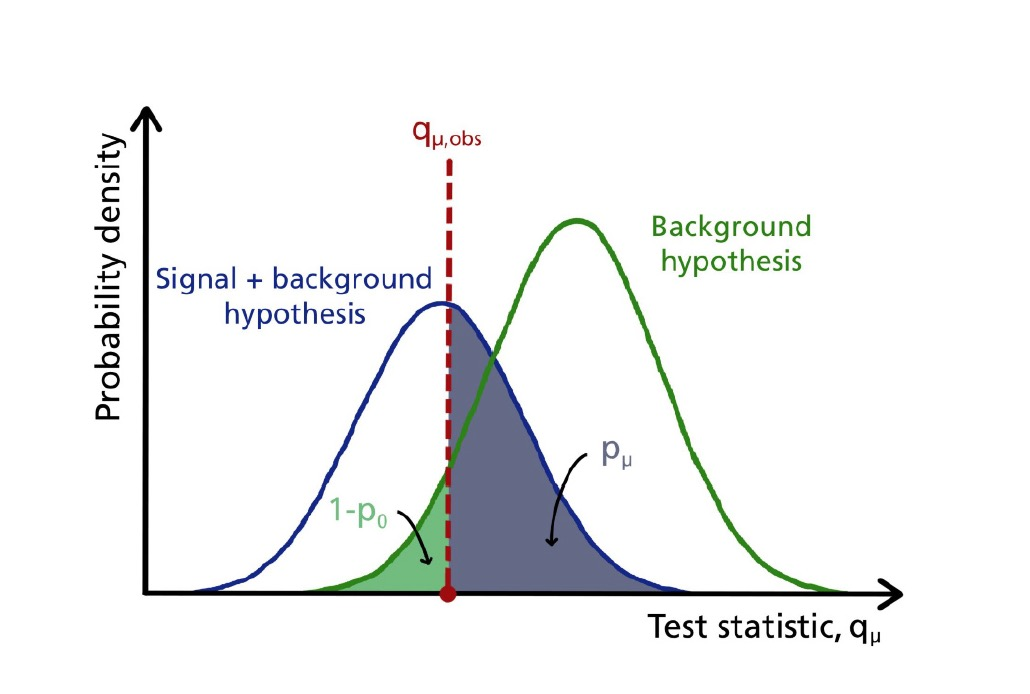
\includegraphics[width=0.75\textwidth]{figuresDijet/10-LimitSettingResults/CLs.jpg}
        \caption{用CL$_\text{s}$方法对信号强度$\mu$设置$95\%$的置信度上限,用图示表示各个变量。}
        \label{fig:CLs}
\end{figure}


这个分析当中,得到的信号强度$\mu$的上限会转换为给定积分亮度和数据下信号$\sigma\times A \times BR$或者$\sigma\times A \times \epsilon \times BR$的$95\%$置信度上限:
\begin{equation} 
\label{eq:Limit8}
\sigma\times A \times \epsilon \times BR =\frac{\mu\times N_s}{L}
\end{equation}
其中$\sigma$是信号的散射截面,A是接收度,BR是衰变两个jet的分支比,$\epsilon$是b-jet标定效率,
$N_s$是总的信号事例数,L是总积分亮度。
统计检验量的概率分布函数可以通过称为渐近近似的解析渐近公式来近似描述~\cite{Cowan:2010js},
它能大大减少计算上限所需要的时间,这里我们用2015年和2016年ATLAS收集的总积分亮度为36.1$fb^{-1}$的数据和$q^*$信号对这种渐近近似方法进行了验证,
如图~\ref{fig:HistVal}~所示,我们对比了用渐近近似方法得到信号的上限和用传统的产生赝数据的方法得到信号的上限,
并没有发现显著的偏差,因此这个分析采用了渐近近似的方法来描述概率分布函数。
信号散射截面的理论误差没有考虑进来。
为了保证连续性,我们会在已设置了$\sigma\times A \times BR$上限的质量点之间进行连续的对数插值。
对于我们考虑到的信号模型,在信号质量处,新粒子的耦合强度要比微扰QCD项的尺度大得多,
因此其与QCD的干涉项可以被忽略。

\begin{figure}[!thbp]
  \begin{subfigure}{.5\textwidth}
  \centering
  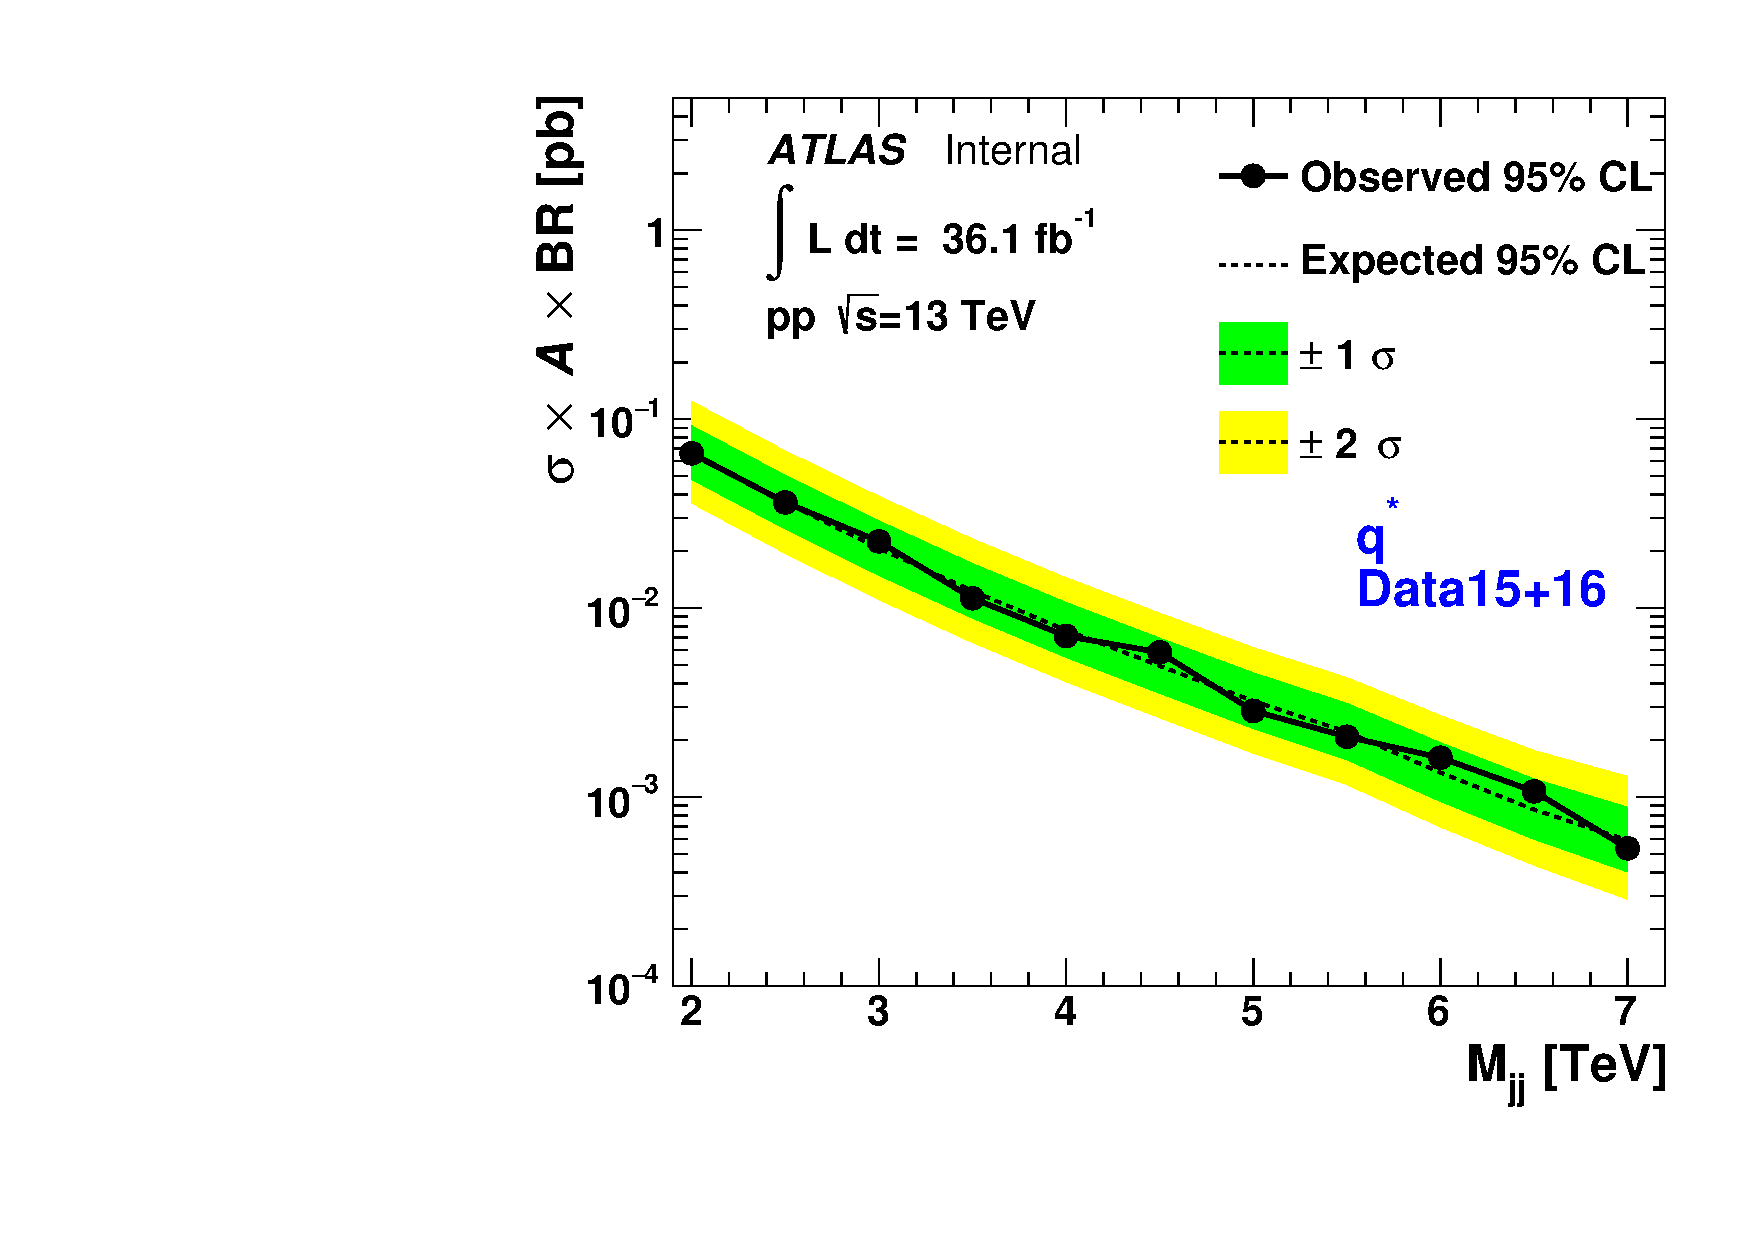
\includegraphics[width=0.9\textwidth]{figuresDijet/Appendix-HF/dijet_qStar_limit_asy.pdf}
  \caption{}
  \end{subfigure}
  \begin{subfigure}{.5\textwidth}
  \centering
  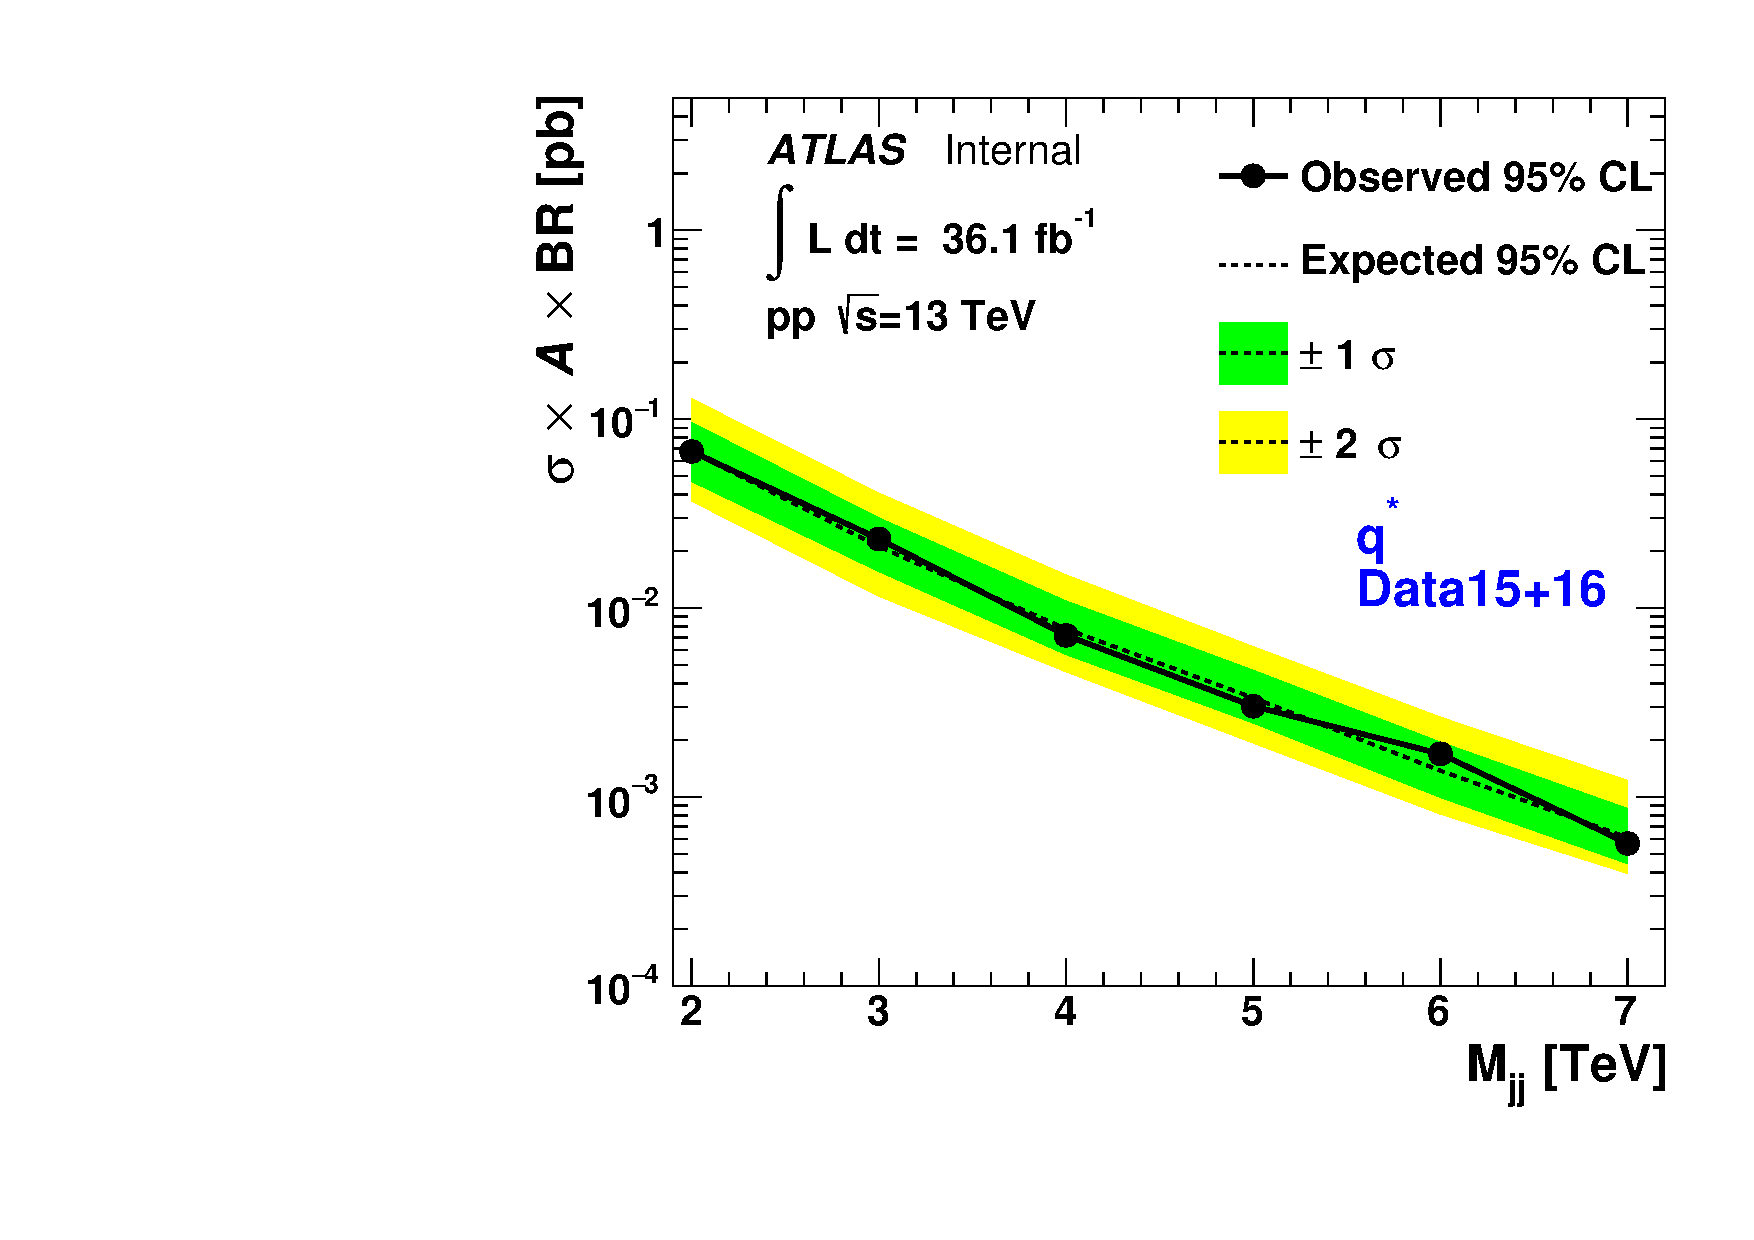
\includegraphics[width=0.9\textwidth]{figuresDijet/Appendix-HF/dijet_qStar_limit1.pdf}
  \caption{}
  \end{subfigure}
\newline
  \begin{subfigure}{.99\textwidth}
  \centering
  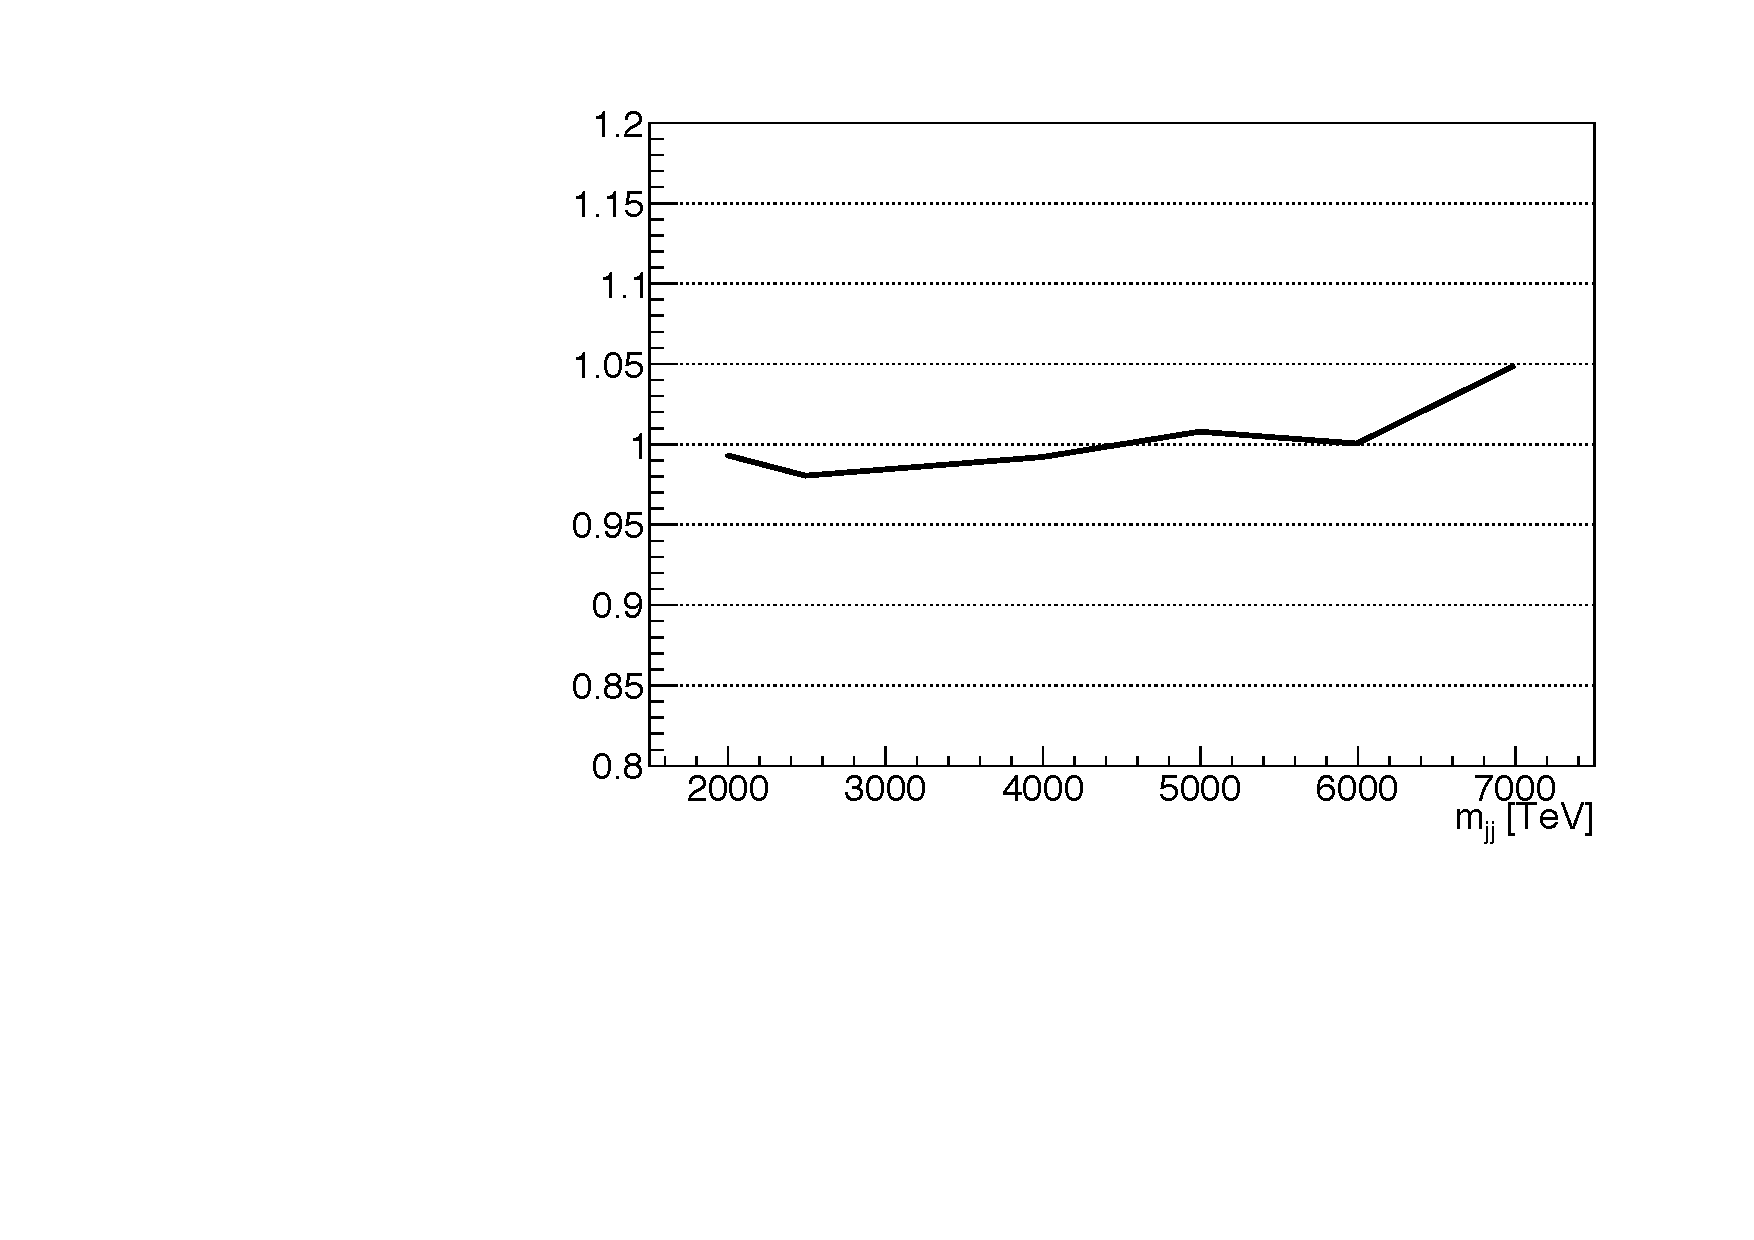
\includegraphics[width=0.5\textwidth]{figuresDijet/Appendix-HF/Ratio.pdf}
  \caption{}
  \end{subfigure}
  \caption{
  上限设置中渐近近似方法的有效性验证。(a) 使用渐近近似方法得到的$95\%$置信度上限;(b) 使用赝数据得到的$95\%$置信度上限;(c) 两种结果中期望上限的比值。
}
\label{fig:HistVal}
\end{figure}

\subsection{上限设置结果} 
\label{sec:DijetSig2}
在全包含信号区,我们对信号$\sigma\times A \times BR$设置了排除上限。
得到的$q^*$、$QBH$、$W'$和$W^*$信号的排除上限如图~\ref{fig:inclusive}~所示,
图中黑色实线表示我们观测到的$95\%$置信度排除上限,
黑色的虚线表示预期的$95\%$置信度排除上限,
绿色和黄色的区域表示相应的$\pm \sigma$和$\pm 2\sigma$误差带,
蓝色的虚线对应于理论排除限。

\begin{figure}[!thbp]
  \begin{subfigure}{.5\textwidth}
  \centering
  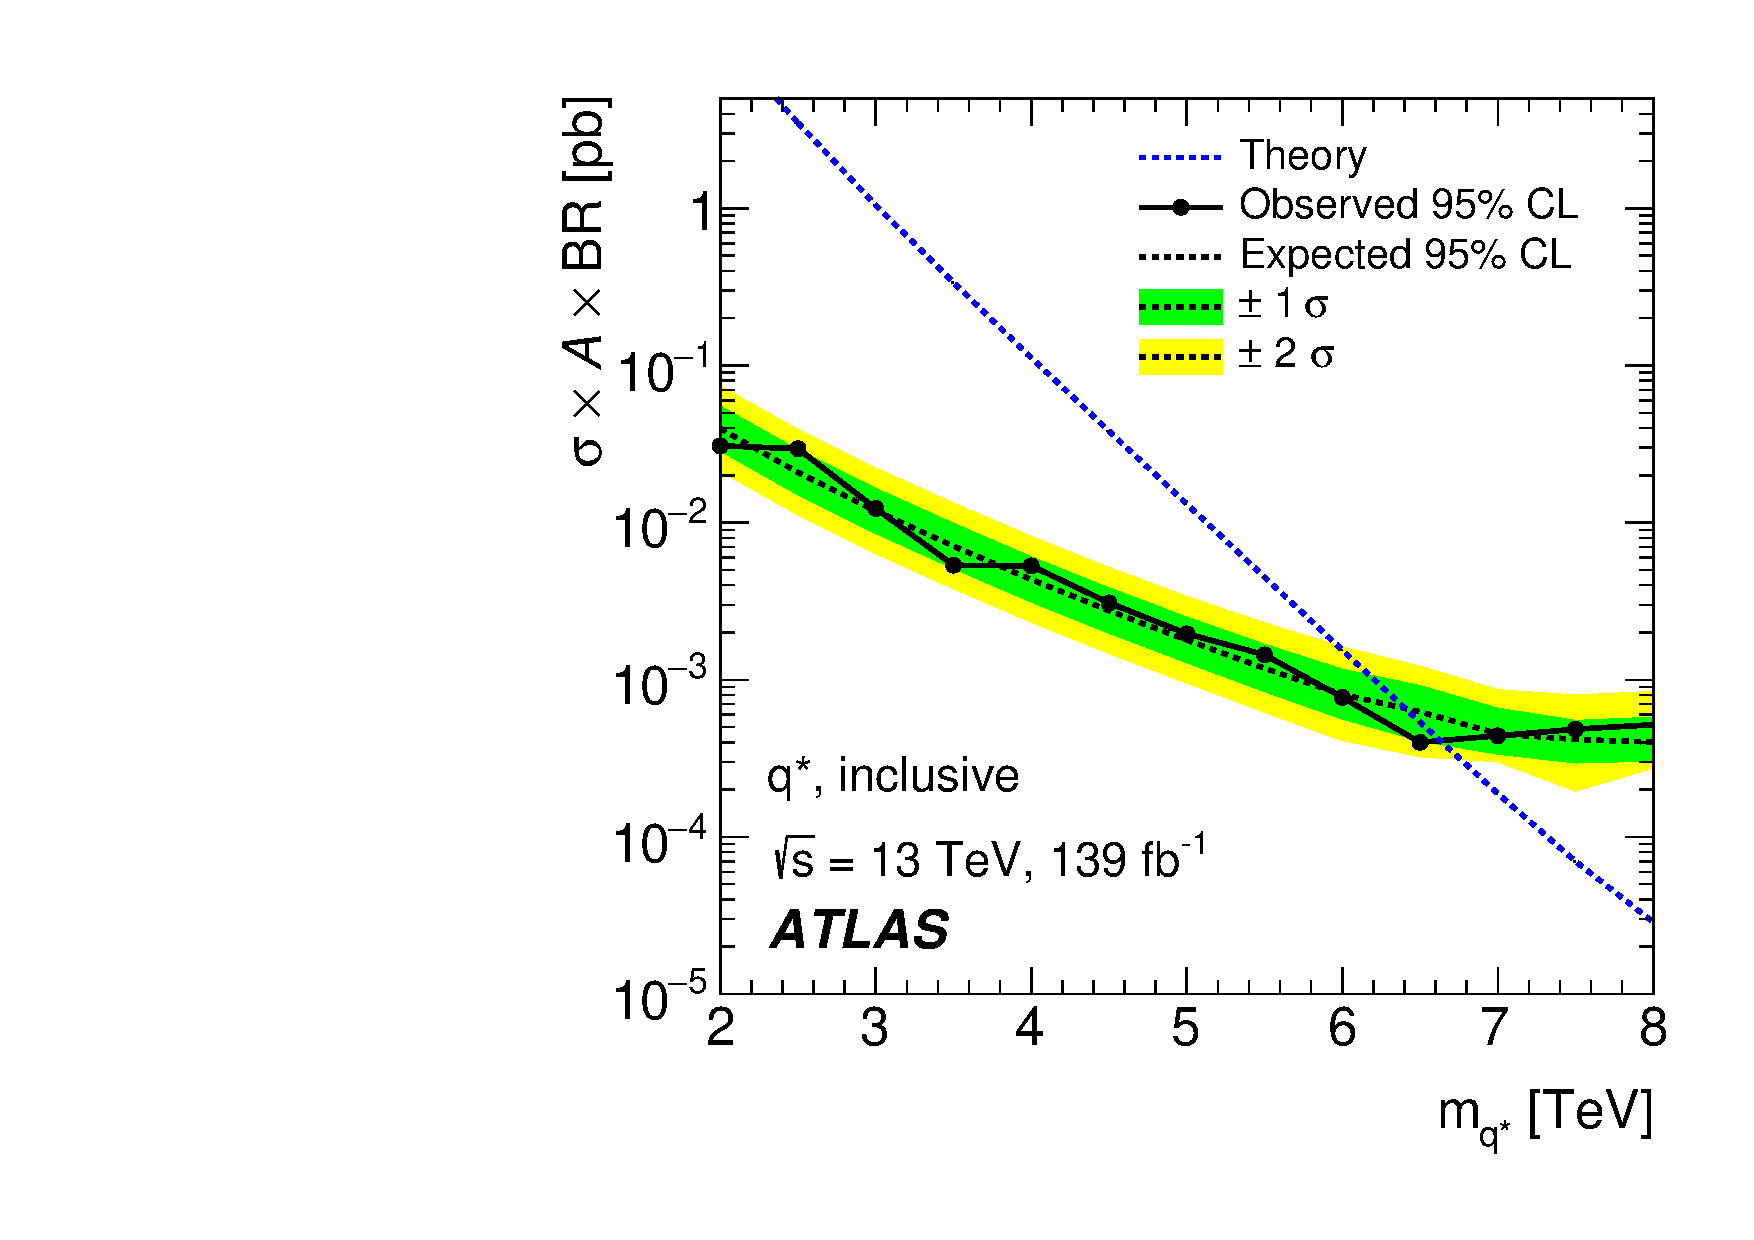
\includegraphics[width=0.9\textwidth]{figs/fig_04a.pdf}
  \caption{}
  \end{subfigure}
  \begin{subfigure}{.5\textwidth}
  \centering
  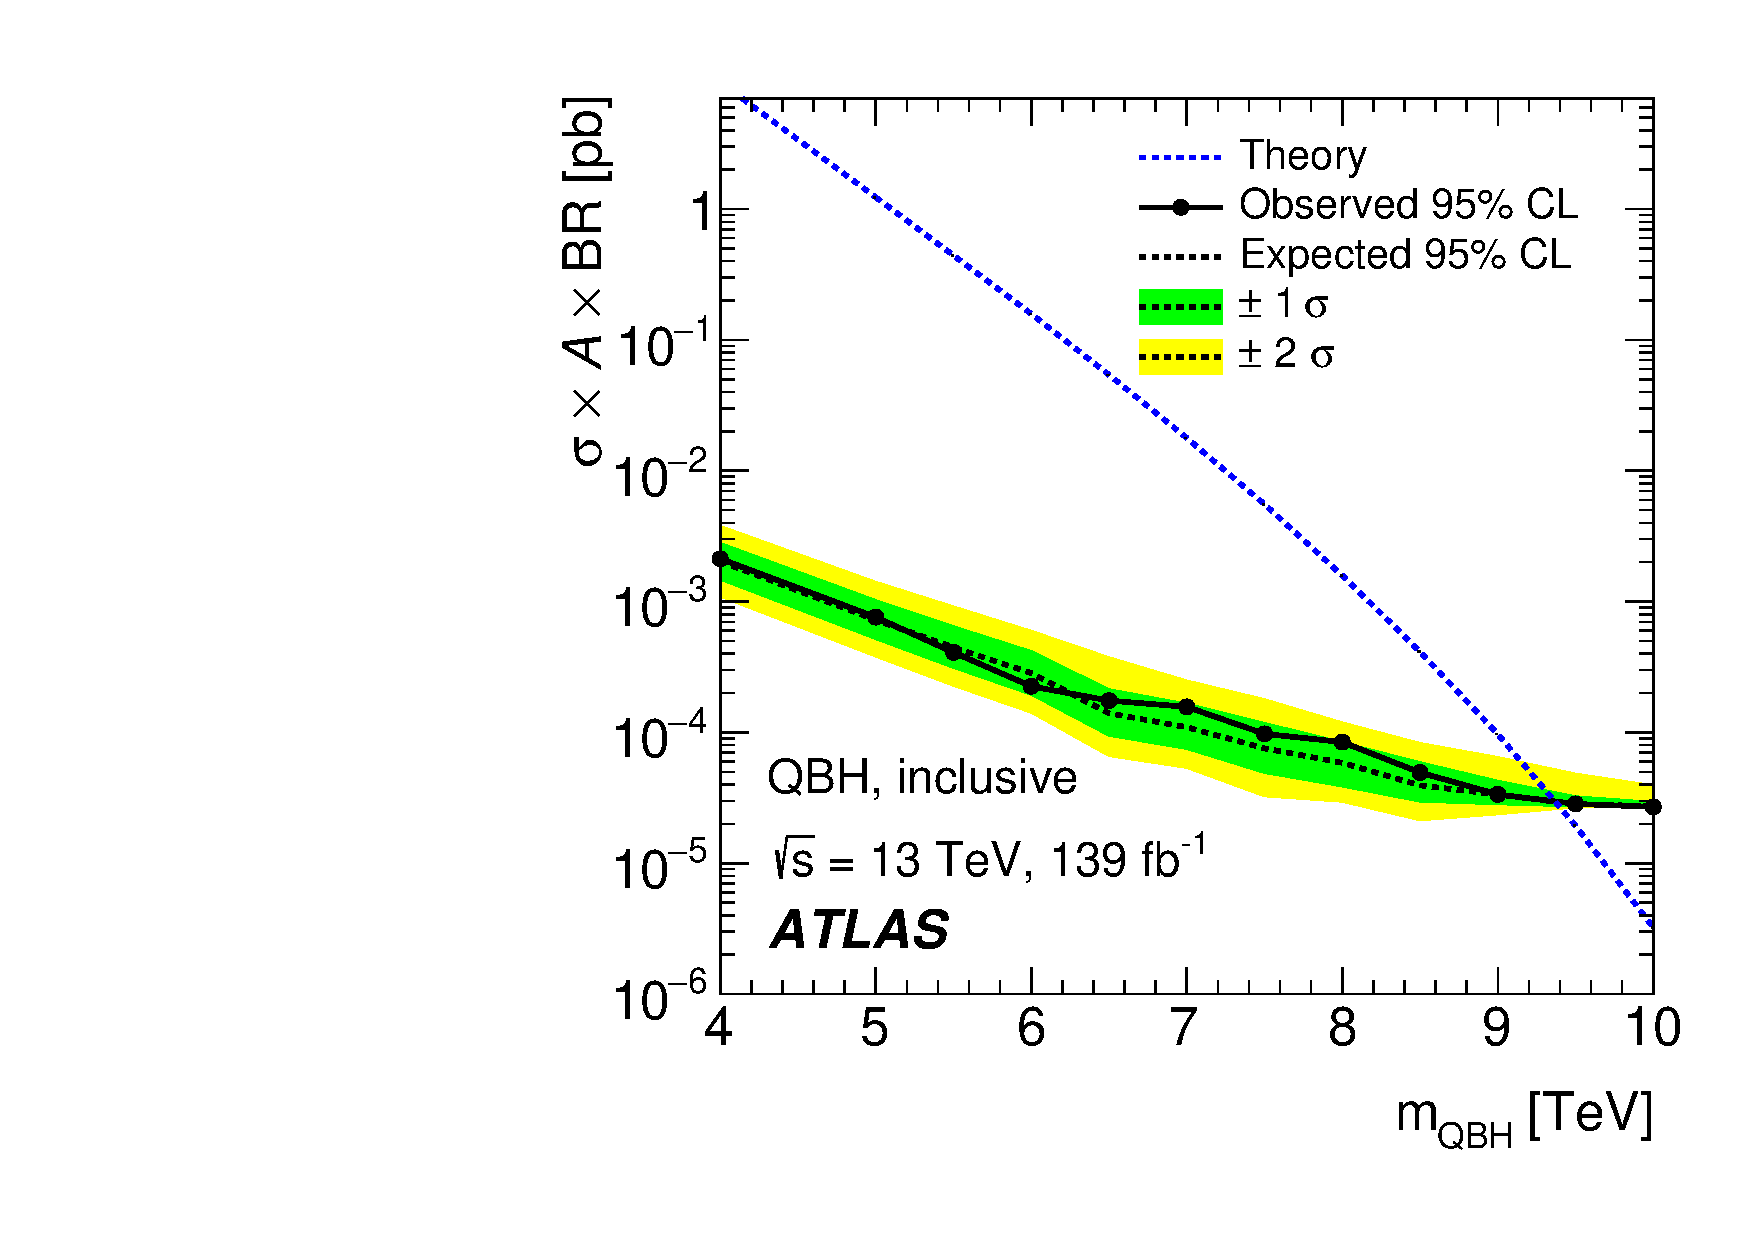
\includegraphics[width=0.9\textwidth]{figs/fig_04b.pdf}
  \caption{}
  \end{subfigure}
\newline 
  \begin{subfigure}{.5\textwidth}
  \centering
  \includegraphics[width=0.9\textwidth]{figs/fig_04c.pdf}
  \caption{}
  \end{subfigure}
  \begin{subfigure}{.5\textwidth}
  \centering
  \includegraphics[width=0.9\textwidth]{figs/fig_04d.pdf}
  \caption{}
  \end{subfigure}
  \caption{
  全包含信号区中,不同信号$\sigma\times A \times BR$的$95\%$置信度上限随着信号质量的变化:(a) $q^*$;(b) QBH;(c) $W'$;(d) $W^*$。
  图中还显示了预期的上限和相应的$\pm \sigma$和$\pm 2\sigma$误差带。
}
\label{fig:inclusive}
\end{figure}



图~\ref{fig:zprime}~展示的是对轻子末态禁闭的DM $Z'$的约束,
此处是DM $Z'$模型的耦合常数$g_q$即$g_{SM}$的上限,所模拟的DM $Z'$信号质量和耦合常数$g_q$的间隔分别为$0.5TeV$和$0.05$。
通过先在$g_q$之间进行插值然后在$Z'$质量之间进行插值,我们在点与点之间绘制一条平滑的曲线。
在给定的质量点,信号散射截面会随着$g_q$的增加而增大,因此左上未被填充的区域将会被排除。

\begin{figure}[tbp]
\centering
\includegraphics[width=0.49\textwidth]{figs/fig_05.pdf}
\caption{
 全包含信号区中,DM $Z'$信号中耦合常数$g_q$即$g_{SM}$的$95\%$置信度上限随着信号质量的变化。
 图中还显示了预期的上限和相应的$\pm \sigma$和$\pm 2\sigma$误差带。
}
\label{fig:zprime}
\end{figure}


在1b和2b信号区,我们对信号$\sigma\times A \times \epsilon \times BR$设置了排除上限。
图~\ref{fig:1b}~展示的是1b信号区的$b^*$信号的排除上限,然后图~\ref{fig:2b}~展示的是2b信号区的$Z'$和Kealuza-Klein引力子信号的排除上限。


\begin{figure}[tbp]
\centering
\includegraphics[width=0.49\textwidth]{figs/fig_06.pdf}
\caption{
  1b信号区中,$b^*$信号$\sigma\times A \times \epsilon \times BR$的$95\%$置信度上限随着信号质量的变化。
  图中还显示了预期的上限和相应的$\pm \sigma$和$\pm 2\sigma$误差带。
}
\label{fig:1b}
\end{figure}

\begin{figure}[!thbp]
  \begin{subfigure}{.5\textwidth}
  \centering
  \includegraphics[width=0.9\textwidth]{figs/fig_07a.pdf}
  \caption{}
  \end{subfigure}
  \begin{subfigure}{.5\textwidth}
  \centering
  \includegraphics[width=0.9\textwidth]{figs/fig_07b.pdf}
  \caption{}
  \end{subfigure}
\newline 
  \begin{subfigure}{.99\textwidth}
  \centering
  \includegraphics[width=0.5\textwidth]{figs/fig_07c.pdf}
  \caption{}
  \end{subfigure}
\caption{
  2b信号区中,不同信号$\sigma\times A \times \epsilon \times BR$的$95\%$置信度上限随着信号质量的变化:
  (a) DM $Z' \to b\bar{b}$;(b) SSM $Z' \to b\bar{b}$;(c) KK $G \to b\bar{b}$, $k/\overline{M}_\text{PL}=0.2$。
  图中还显示了预期的上限和相应的$\pm \sigma$和$\pm 2\sigma$误差带。
}
\label{fig:2b}
\end{figure}



表~\ref{tab:limits}~总结了每个基准信号模型的质量下限。
对于DM $Z'$模型,在信号质量1.5TeV为左右,来自2b信号区的约束与全包含信号区的约束是相当的,
但是在高质量区,由于b-jet标定效率的损失,使得来自2b信号区的约束比全包含信号区的约束要弱。
对于衰变到b夸克末态分支比更大的新共振态,1b和2b信号区将会具有更高的灵敏度。


\begin{table}[htbp]
  \caption{ 在$95\%$置信度下,各个基准信号的质量下限的总结。}
  \centering
  \begin{tabular}{l|c|c|c}
    \hline\hline
    \multirow{2}{*}{Category} & \multirow{2}{*}{Model} & \multicolumn{2}{c}{Lower limit on signal mass at 95\% CL} \\ 
    & & Observed & Expected \\\hline
    \multirow{6}{*}{Inclusive} & $q^*$ & 6.7 TeV & 6.4 TeV  \\
    & QBH & 9.4 TeV  & 9.4 TeV \\
    & $W'$ & 4.0 TeV & 4.2 TeV  \\
    & $W^*$   & 3.9 TeV & 4.1 TeV \\
    & DM mediator $Z'$, $g_\text{q}=0.20$ & 3.8 TeV & 3.8 TeV \\
    & DM mediator $Z'$, $g_\text{q}=0.50$ & 4.6 TeV & 4.9 TeV \\\hline
    $1b$ & $b^*$ & 3.2 TeV & 3.1 TeV \\\hline
    \multirow{4}{*}{$2b$} & DM mediator $Z'$ $g_\text{q}=0.20$ & 2.8 TeV  & 2.8 TeV \\
    & DM mediator $Z'$, $g_\text{q}=0.25$ & 2.9 TeV  & 3.0 TeV \\
    & SSM $Z'$, & 2.7 TeV & 2.7 TeV \\
    & graviton, $k/\overline{M}_\text{PL}=0.2$ & 2.8 TeV & 2.9 TeV \\\hline\hline
  \end{tabular}
  \label{tab:limits}
\end{table}


在图~\ref{fig:gauss}~中,我们也对能在dijet末态不变质量谱$m_{jj}$上产生一个共振峰的一般高斯信号的有效散射
截面$\sigma\times A \times BR$或$\sigma\times A \times \epsilon \times BR$设置了排除上限,
这里的BR是指信号衰变末态为两个jet所占的分支比,在1b和2b信号区,上限中还包含了b-jet标定效率$\epsilon$。
并且,我们在探测器重建的水平上测试了各种不同信号质量和宽度的高斯信号模型,
信号宽度的范围从接近探测器分辨率大约$3\%$的相对宽度变化到$15\%$的相对宽度,由于更宽信号的出现会显著影响由滑动窗口拟合方法估计的本底,因此这里并未考虑更宽的信号,
同时我们引入了一个基于MC的转移矩阵来连接粒子层面的观测值和重建层面的观测值,并用它来补偿探测器对粒子层面信号响应的影响~\cite{EXOT-2016-21}。
在全包含信号区,质量为1.5TeV的高斯信号的有效散射截面的排除上限大约在30-70fb之间,质量为6TeV的高斯信号的有效散射截面的上限大约在0.08-0.2fb之间。
在1b和2b信号区,高斯信号质量为1.5TeV时,有效散射截面的上限分别约在5-20fb和4-6fb之间。
在1b信号区,最高的质量点在5TeV,对应的上限在0.1-0.4fb之间,在2b信号区,最高的质量点在4.5TeV,对应的上限约为0.04fb。



\begin{figure}[!thbp]
  \begin{subfigure}{.5\textwidth}
  \centering
  \includegraphics[width=0.9\textwidth]{figs/fig_08a.pdf}
  \caption{}
  \end{subfigure}
  \begin{subfigure}{.5\textwidth}
  \centering
  \includegraphics[width=0.9\textwidth]{figs/fig_08b.pdf}
  \caption{}
  \end{subfigure}
\newline 
  \begin{subfigure}{.99\textwidth}
  \centering
  \includegraphics[width=0.5\textwidth]{figs/fig_08c.pdf}
  \caption{}
  \end{subfigure}
  \caption{
  一般高斯信号的$95\%$置信度上限随着信号质量$m_{X}$的变化:(a) 全包含信号区;(b) 1b信号区;(c) 2b信号区。
  这里考虑了相对宽度从$0\%$到$15\%$的高斯信号,并且在1b和2b信号区,上限中还包含了b-jet标定效率$\epsilon$。
  其中宽度为$0\%$的高斯信号对应于相对宽度小于探测器分辨率的高斯信号,而对于$15\%$的高斯信号,当信号与$m_{jj}$尾部开始重叠时,上限将被截断。
}
\label{fig:gauss}
\end{figure}


与ATLAS合作组上一轮分析用贝叶斯方法~\cite{Caldwell:2008fw}的得到的结果~\cite{EXOT-2016-33}相比,此分析受益于b-jet标定算法DL1r和与之相关的系统误差的显著改进。
图~\ref{fig:money_analysis}~展示的是DM $Z'$信号$\sigma\times A \times \epsilon \times BR$的$95\%$置信度上限在当前和之前的期望值,
图~\ref{fig:money_analysis}~中蓝色虚线表示在假定之前的分析策略和其系统误差不变的情况下,由之前$36.1fb^{-1}$的结果按统计量放大到当前$139fb^{-1}$数据量的预期上限值,
在我们所研究的质量范围内,除去积分亮度增加的因素,预期上限值相对于之前的预期上限值提升了最大有3.5倍。

\begin{figure}[htbp]
\centering
\includegraphics[width=0.6\textwidth]{figs/fig_09.pdf}
\caption{
DM $Z'$信号$\sigma\times A \times \epsilon \times BR$的$95\%$置信度上限在当前和上一轮分析~\cite{EXOT-2016-33}的期望值,
蓝色虚线表示在假定之前的分析策略和其系统误差不变的情况下,由之前$36.1fb^{-1}$的结果按统计量放大到当前$139fb^{-1}$数据量的预期上限值。
得益于b-jet标定算法DL1r和与之相关的系统误差的显著改进,使得上限有着显著提升。
}
\label{fig:money_analysis}
\end{figure}



\section{本章小结} 
\label{sec:DijetCon}

利用由LHC上ATLAS探测器在2015年到2018年记录的质心系能量为$\sqrt{s}=13TeV$的总积分亮度为$139fb^{-1}$的质子-质子对撞数据,我们通过分析事例中两个最高横动量jet的不变质量谱$m_{jj}$在全包含、1b和2b三个信号区中搜寻了能衰变到两个jet的新共振态,在标准模型所预言的用数据驱动方法估计的平滑下降的本底上没有发现显著的新物理信号。
并对各种信号模型和一般的高斯信号进行了约束。比如,在$95\%$置信度下质量低于$6.7TeV$的激发态$q^*$信号被排除,对于$SSM Z'$模型,在$95\%$置信度下质量低于$2.7TeV$的信号被排除。
相对于上一轮类似的分析,和b-jet标定相关的两个信号区得益于在高横动量下b-jet标定算法的显著改进,除了因积分亮度的增加带来的提升之外,我们的灵敏度在此基础上有了更大的提升。





